\documentclass[12pt]{article}
%% \title{Energy and Growth, History and Dynamics}
%\title{Economic development with unlimited supplies of energy:
%\\The English Industrial Revolution and modern economic growth}

\title{The rise and fall (?) of (industrial) capitalism \\%for 1501 URPE ASSA
Prepared for the ASSA URPE conference\\
Boston, Massachusetts\\
January 2015\\
}
\author{
	Stephen C. Bannister\\
	Department of Economics\\
	University of Utah\\
	Salt Lake City, Utah 84112\\
	USA\\
	801-581-7481\\
	\href{mailto:steve.bannister@econ.utah.edu}{steve.bannister@econ.utah.edu}\\
	}

%\date{Drafts May 2012,}
\date{}
\usepackage[latin1]{inputenc}
%\usepackage[english]{babel}
\usepackage{amsmath}
\usepackage{amsfonts}
\usepackage{txfonts}
\usepackage{amssymb}
\usepackage{pgfpages}
\usepackage{booktabs}
\usepackage{longtable}

\usepackage{chngpage}
%\usepackage{pdfpages}
\usepackage{graphicx}
\usepackage[lofdepth,lotdepth,position=bottom]{subfig}
\usepackage{caption}
%\usepackage{draftwatermark}
\usepackage[round]{natbib}

\usepackage{verbatim}
%\usepackage{underscore}
\linespread{1.6}	% remove for single, 1.3 for 1.5 and 1.6 for 2.0. use this setting for print editing

\usepackage{glossaries}

\graphicspath{{../images/}}

%\textwidth{7.5in}
\addtolength{\textwidth}{1.0in} 
\addtolength{\oddsidemargin}{-0.5in} 
\addtolength{\evensidemargin}{-0.5in} 
\addtolength{\textheight}{1.25in}
\addtolength{\topmargin}{-0.75in}

\usepackage{tocloft}

\usepackage{hyperref}

\makeglossaries

\loadglsentries{glossary.tex}

%\setcounter{secnumdepth}{4}%to number paragraphs so can ref them?

\begin{document}

%\SetWatermarkLightness{0.93}
%\SetWatermarkScale{1}

	\maketitle
%	\nocite{*}
%	\bibliographystyle{E:/LaTeX-Portable/MikTex-Portable/bibtex/bst/base/IEEEanot}

%	\bibliographystyle{E:/LaTeX-Portable/MikTex-Portable/bibtex/bst/base/plain-annote}
%	\bibliographystyle{plain}

\newcommand{\listequationsname}{List of Equations}
%\newlistof{myequations}{equ}{\listequationsname}
\newlistof{myequations}{equ}{\listequationsname}
\newcommand{\myequations}[1]{%
\addcontentsline{equ}{myequations}{\protect\numberline{\theequation}#1}\par}


	\begin{abstract}
	My work toward understanding attempts at industrial revolutions, both successful and failed, as primarily energy-consumption revolutions and understanding their structure, leads me to a new understanding of the origins of industrial capitalism as an outcome of demand and supply shifts driven by both macro- and micro-economic forces.  This work can be placed firmly in the historical materialism tradition and extends it. I also situate this in the tradition of endogenous institutions. The work uses Sung China ( Northern Sung dynasty, 960 -- 1127 CE ) and Early Modern England as case studies.
	
	As social scientists, if we hope to help bend the curve of history toward positive institutional change, we must understand the roots of the pervasive institution we call industrial capitalism, which continues to influence our personal and collective lives in many ways.
	
	My conclusion is that it is possible to eliminate much of the ``bad'' of industrial capitalism, but doing so will require a specific development path following historical materialism precepts: we need a radical change in the means of production, the technologies we build to meet our material needs and the institutions they imply. Such change must cause a dramatic reduction in the need for accumulated capital; in the language of economics, we must reduce the demand for capital to overcome its negative effects or externalities on ``the non-invidious recreation of community,'' a quote from Marc R. Tool \citep{bokus_institutional_2014}.
	
	Describing a technological development path that honours revealed economic fundamentals while meeting material needs with reduced capital demand is feasible; to do so without understanding the paths that led to our present state makes that task unnecessarily difficult. I hope to contribute to making the rise of industrial capitalism usefully understandable, and thus the probability of diminishing it feasible.

	\end{abstract}

\begin{comment}	
\section*{outline}	
\begin{itemize}
\item Historical materialism
\item Endogenous institutions. Large and permanent cultural and institutional changes are caused by large and permanent economic changes.
\item Industrial revolutions -- two main stages -- require industrial capitalism
\item Demand for capital -- coal, steam
\item Supply of capital -- merchant capitalism, nobility
\item Sung China -- supply, insufficient demand
\item IR England -- supply and sufficient demand, an energy revolution
\item Future energy revolutions -- implications for capital -- two possible paths
\item describe current state of capitalism (solar farms as an example)
\item describe a path which reduces demand for capital, thus causes capitalism to whither
\end{itemize}
\end{comment}


\section{Introduction}	%last

This paper explores the idea that institutional changes, at least important ones, are primarily endogenous, and especially so to major economic changes. While this a very richly explored area, starting with the historical materialism school that Karl Marx fathered, I plan to contribute by extending the apparatus to microeconomic explanations, providing further macroeconomic insights, and examining historical events. My topic is large: the origin of industrial capitalism, with hints about its future.

I view industrial capitalism as a mode of production consisting of large, centrally controlled accumulations of capital used to finance the means of production for commodities destined for market, using largely wage-labor, and characterized by large scale production, accumulation, and limited private ownership.

If my basic thesis is to be seen as useful, I must show that the rise of industrial capitalism was caused by a sufficiently large economic change; fortunately, many economic and other historians see as I do that the English Industrial Revolutions (henceforth EIR) was sufficiently large, perhaps the largest economic event in tens of millennia. The contemporaneous timing of the rise of industrial capitalism with the EIR is highly suggestive.

In other work, I claim that the EIR was primarily an energy revolution. As we will see, using comparative stories of Sung China and England, I can narrate how the EIR originated primarily in changes in demand regimes and the energy economy, and how those changes led directly to the rise of industrial capitalism from the prior regime of merchant capitalism. The Sung Chinese started, but failed to complete, this journey while England succeeded.

I agree with Robert Brenner \citep{brenner_agrarian_1976} and E. A. Wrigley \citep{wrigley_continuity_1988}	that the large changes we call the English Industrial Revolution have a prime mover, or essentialist, explanation. I here part with Brenner's class-relations explanation, and extend Wrigley's energy transition explanation.

At best, this paper will outline a suggestion, perhaps a framework, for future research; this space is certainly one of the most well travelled among economic historians, classical institutional economists, New Institutional economists, World-Systems practitioners, and others.

\section{Literature background}

\subsection{Historical Materialism}

I will not extensively review historical materialism, except in summary for those who may have never been exposed to the idea. The kernel is that changes in material conditions such as technology and productive capacity are primary to changes in socioeconomic institutions and organization. Quoting Marx from ``A Contribution to the Critique of Political Economy'' \citep{marx_contribution_1904}:

\begin{quote}
``In the social production of their existence, men inevitably enter into definite relations, which are independent of their will, namely relations of production appropriate to a given stage in the development of their material forces of production \ldots 
\begin{comment}
 The totality of these relations of production constitutes the economic structure of society, the real foundation, on which arises a legal and political superstructure and to which correspond definite forms of consciousness. The mode of production of material life conditions the general process of social, political and intellectual life. It is not the consciousness of men that determines their existence, but their social existence that determines their consciousness. 
\end{comment}
At a certain stage of development, the material productive forces of society come into conflict with the existing relations of production or-- this merely expresses the same thing in legal terms -- with the property relations within the framework of which they have operated hitherto. From forms of development of the productive forces these relations turn into their fetters. Then begins an era of social revolution.'' 
\begin{comment}
The changes in the economic foundation lead sooner or later to the transformation of the whole immense superstructure. In studying such transformations it is always necessary to distinguish between the material transformation of the economic conditions of production, which can be determined with the precision of natural science, and the legal, political, religious, artistic or philosophic -- in short, ideological forms in which men become conscious of this conflict and fight it out. Just as one does not judge an individual by what he thinks about himself, so one cannot judge such a period of transformation by its consciousness, but, on the contrary, this consciousness must be explained from the contradictions of material life, from the conflict existing between the social forces of production and the relations of production.''
\end{comment}

\end{quote}

%% insert here institutions -- conservative, reactionary, repressive. e.g. Koreas

\subsection{Recent institutional endogeneity theory}

Supporting Marx, in my view, modern work arising from agricultural economics offers theories of technological and institutional change induced by changes in relative resource endowments and technology. This work is founded in microeconomics. Ruttan and Hayami have a good exposition \citep{ruttan_toward_1984}. 
%\footnote{Ruttan, Vernon W., and Yujiro Hayami. ``Toward a Theory of Induced Institutional Innovation.'' Journal of Development Studies 20, no. 4 (1984): 203-223. doi:10.1080/00220388408421914.}

Whether Marx or Ruttan, macro or micro, sociology or economics, the stories are the same: economic changes cause institutional and cultural changes. There is a very large body of literature, for example the Western exceptionalism literature including Weber, that argues this causality differently. I do not review that work here, simply appealing to the fact that the contemporaneous people had either no or very dim knowledge of what the EIR was and could not therefore have foreknowledge of institutions that would be required for its success. Further, hypothesizing endogenous institutional change ahead of economic changes strains logic.

\subsection{Jan de Vries from Early Modern Capitalism -- a survey}
Jan de Vries, in a seminal chapter in Maarten Prak's edited volume ``Early Modern Capitalism -- Economic and social change in Europe, 1400--1800,'' clearly defines the great debates among the various disciplines and schools who continue attempting to explain the English Industrial Revolution.

de Vries' chapter, ``Economic growth before and after the Industrial Revolution -- a modest proposal,'' explains the contours of the debates, and in the end argues for a broad historical approach rather than one dominated by a particular school of thought \citep{prak_economic_2001}. 

The structure of his thinking is so clarifying that I start with it as an organizing framework in my work here whose goal is to illuminate the rise of industrial capitalism, and investigate its primal cause -- institutions (including culture) or economics; of course both happened, but I wish to see if there is a clear primal driver. I land in a different place than de Vries.


\subsubsection{Different modeling schools produce an ahistorical approach}
de Vries opens by analyzing the problems in past and current approaches: ``Coherent accounts of historical economic growth are difficult to achieve only in part because of the venerable jurisdictional boundaries that have for so long governed the training of professional historians'' \citep[p.177]{prak_economic_2001}. This causes different story tellers for eighteenth (early modern) and nineteenth (late modern) histories, and thus at least the potential for different stories.

de Vries continues: ``One might suppose that what historians tear asunder with their conventions of periodization, economists would stitch together with the healing balm of theory'' \citep[p.177]{prak_economic_2001}. But, before the neo-classical era, economists applied classical models with some binding constraint, usually land, whether the modeller followed Smith, Malthus, or Ricardo in details. Later neo-classical modellers assumed constant returns to scale, substitutability at all margins, and technologies freely available to all, and thus told a story abstracting from all time and space -- no history, no geography. And thus he introduces his case for a more integrative approach to fix the rifts in both historical and economic story-telling, an approach I attempt to extend.

\subsubsection{The Industrial Revolution}
de Vries examines the revisionist version of the EIR, and then proceeds to examine the ``bookends.'' Here, I summarize de Vries' key arguments:

Commenting on the commonly-held neo-classical model's ``bookends'' of the EIR, meaning the neo-Malthusian model that preceeds it, and the Kuznetsian model of modern economic growth that follows it, a unitary growth model with a single long term trend, de Vries accepts the revisionist criticisms from many including \cite{mokyr_editors_1993}, \citet[p.26]{jones_growth_1988}, and \cite{crafts_output_1992}. The revisionists claim the EIR covered a longer period, and a slower rate of growth than Kuznet's version. But de Vries does not fully dismiss his bookends, instead appealing to the complexity of the event and saying that we must revise those models. I agree. Along they way, de Vries dismisses as un-historical and un-empirical the neo-classical ``Solow'' convergence models. While complex, my view is that most narratives are also un-economic, a puzzling oversight given the people telling the stories. Again, I hope to contribute to correcting this oversight.

\subsubsection{Modern economic growth}
First, de Vries sketches the contours of modern economic growth, post Industrial Revolution, using the seminal empirical work of Simon Kuznets, Phyllis Deane and W. A. Cole, and Angus Maddison. He supports the empirics with the neo-classical growth theory represented by Robert Solow's work. These works unarguably describe a structural break from the prior rate of economic growth, supported by a growth theory that demands technological change for its growth engine. The facts clearly support this story.

\subsubsection{The neo-Malthusian model -- pre-industrial growth}
Next, de Vries outlines the pre-Industrial Revolution neo-Malthusian models. He cites a large number of contributors including Fran\c{c}ois Simiand, Wilhelm Abel, Ferdnand Braudel, Michael Postan, E. H. Phelps Brown and Sheila Hopkins, B. H. Slicher van Bath, Emmanuel Le Roy Ladurie, and importantly, the team of E. A. Wrigley and R. S. Schofield. The consistent essence of this model is that movement in populations, fuelled by sexual relations, is the dominant economic relationship and is always constrained by a more-or-less fixed supply of land to feed the population and an agricultural technology at it's frontier \citep[p.181]{prak_economic_2001}. Pausing the de Vries narrative, I turn to that of E. A. Wrigley on the Malthusian world -- with Wrigley bringing clarity to that story.

E. A. Wrigley models this world with useful components; he describes the world in, among other references, ``People, Cities and Wealth.'' The main components of the Wrigley model include living standards (most often represented as Gross Domestic Product per capita), nuptiality (marriage) rates and ages, and fertility rates. In the neo-Malthusian world, before about 1880 in England, there is a strong positive correlation between living standards and nuptiality rates, and subsequently a very strong positive correlation between nuptiality rates (and age at first marriage) and fertility rates. In this world, as living standards fluctuate upward due typically to exogenous factors such as better weather and crops, more women marry at a younger age, and therefore increasing fertility rates drive up population levels.

Wrigley's (and Scofield's) \citep[p.237]{wrigley_people_1987} major correlations for his neo-Malthusian model for England are summarized as follows:

\begin{table}[h!]
\begin{tabular}{lll}
Factor 1&Factor 2&Sign of correlation\\
\hline \hline
Population increase&Food prices increase&Positive\\
Food price increase&Real income decrease&Negative\\
Real income decrease&Nuptiality decrease&Positive\\
Nuptiality decrease&Fertility decrease&Positive\\
Fertility decrease&Population decrease&Positive\\
\hline
\end{tabular}
\end{table}

\newpage

Thus rising population caused lower living standards and retarded fertility through the nuptiality mechanism. Wrigley claims a different mechanism for China's version of a neo-Malthusian model as in:

\begin{table}[h!]
\begin{tabular}{lll}
Factor 1&Factor 2&Sign of correlation\\
\hline \hline
Population increase&Food prices increase&Positive\\
Food price increase&Real income decrease&Negative\\
Real income decrease&Mortality increase&Negative\\
Mortality increase&Population decrease&Negative\\
\hline
\end{tabular}
\end{table}

Wrigley summarizes the ``Chinese'' version of his model this way: ``Here to balance the books[,] nature audits with a red pencil'' \citep[p.236]{wrigley_people_1987}. This neo-Malthusian variant was not the most pleasant of existences.

The fundamental importance of Wrigley's theories is that they fit the historical data that we know describes the millennia preceding the EIR in terms of population and living standards, and suggest how radically these changed post-Revolution. The history is of increasing total final demand because of gradually rising population and, cyclically, rising living standards. But the rising final demand eventually ran into some constraint or set of constraints that caused living standards to fall. 

Only in the late eighteenth century was this perpetual cycle interrupted, allowing simultaneous increases in both population and living standards. Total final demand started marching inexorably upward and the supply revolution that was the EIR was able to continually match the population's rising desires and incomes for the first time in history.

de Vries further covers, de rigueur, the contributions of Michael Postan and Emmanuel Le Roy Ladurie. These are important contributions; Wrigley, however has both the theory and data that is convincing.

Surveying this extended era of pre-industrial growth, de Vries summarizes that, given the ``revised view of British macro-economic performance during the Industrial Revolution\ldots'' (less than earlier estimates) ``\ldots would appear to required that significant pre-industrial growth took place in the long run'' \citep[p.188-9]{prak_economic_2001}. He cites contributing factors to this secular growth as including institutional development, urbanization, demographic control mechanisms, market expansion, agriculture, industrial organization, and technology. These surely are important developments, but as of yet, there is no primal contributor. That is a defect that de Vries next notes, and I attempt to correct.


\subsubsection{From two models to one}
de Vries approaches the great question, how to explain the miracle of the EIR, by quoting from David Landes \citep{mokyr_fable_1993}: ``In a polemic directed against revisionists of the Industrial Revolution, David Landes excoriates economists in general and Cliometricians in particular for being `passionate seekers after the One Cause, the prime mover.' He (Landes) observes that these methodologically sophisticated economists forget that everything is substitutable and hence nothing is indispensable,'' \ldots and praises the approach of `multiple causation' (189).

de Vries further comments that ``Landes fails to acknowledge that the search of the One Cause of the Industrial Revolution arises from the need to explain the lifting of the great constraint that defines the neo-Malthusian model'' and then invokes Wrigley as a champion of the `essentialist' approach \citep[p.189]{prak_economic_2001}. Indeed.

He then describes the gradualist approach and then, amazingly to me given how far he travelled in this chapter, makes the case for a centrist approach, basically ignoring my reading of Wrigley's core essentialist message in ``Continuity, Chance and Change'' \citep{wrigley_continuity_1988}.

In the remainder of this paper I try to strengthen the essentialist message, which then leads directly to the rise of industrial capitalism. I first develop a very basic theory of the EIR which applies also to China, and perhaps to other pre-modern industrialization attempts such as the Dutch Republic during the sixteenth and seventeenth centuries. If supported, this then is progress toward a general theory of industrial revolutions.

\section{Industrial revolutions}
 In other work, I provide a theory for industrial revolutions, centered on the EIR. There I claim and demonstrate empirically that the EIR was essentially an energy revolution in the strong sense that without the energy revolution there would not have been an event which has come to be called the EIR. 
 
The core elements of this theory are in the Technical Appendix, section \ref{sec:techAppendix}.
 
 Summarized, the story unfolds this way. There was an up-welling of populations and thus total incomes during the Middle Ages; this is temporally related to the Medieval Warming Epoch which increased (likely globally) agricultural yields and influenced institutions and culture. Increased goods and services demand led to increased production in heat-consuming industries such as smelting, metal working, salt making, dyeing, and brewing. Heat consuming industries used mainly wood (sometimes as charcoal) as their energy source. The wood demand deforested neighborhoods, regions, and countries. Wood prices rose dramatically, for example in sixteenth century England. This also affected household uses of wood for heating and cooking.
 
 Producers and households naturally sought alternative energy sources. In England and China, that source was coal. Using coal for heating was not an easy technological transition for many reasons; the full transition was on the order of centuries. In the Dutch Republic, the energy source was peat. The Dutch ran out of peat supplies and their industrialization attempt stalled.
 
 In pre-modern eras, this was the path to an industrial revolution, the transition from an inherently limited energy source, trees, to an essentially unlimited source, coal. Both England and China did this, and further research should show that other areas in addition to the Dutch Republic did as well. But this is only the first step on the path.
 
 The main leap to an industrial revolution, exemplified in the EIR, was learning to substitute the new energy source not just for the heating industries, but through the application to steam-powered devices to supplant human and animal power. This invention unleashed the enormous productivity gains and scale that are the hallmarks and legacy of the EIR.
 
 Of course, I still need to explain what was unique about England, but this is sufficient background to delve into the foundations of industrial capitalism, which was not uniquely English at its roots.
 
\section{The rise of the demand for capital and its supply -- the path to industrial capitalism} 

\subsection{Transition from wood to coal for heating - England}

In the ``real economy'' story of the previous section, we have clues that explain how the demand for capital arose, which when paired with the capital supply story, will give us a picture of the economic foundations for that institution. First the demand side, and first for England.

John Nef plays an important role in this story. Nef, a University of Chicago historian, produced in 1932 a two-volume work titled ``The Rise of the British Coal Industry.'' This is a little-cited work in recent scholarship; scholars should seek it out -- this is as definitive a work as one could hope for \citep{nef_rise_1932}.
%\footnote{Nef, John Ulric. The Rise of the British Coal Industry. 1St Edition. George Routledge \& Sons, 1932.}

In Volume I, Part IV, Chapter I, Nef lays out the case for the necessity of the development of capitalism to support the level of investment needed in the nascent coal industry. Nef dates the start to the mid-sixteenth century, along with the rise of using coal as a heating fuel. He discusses  that the division of labor in the mining and transportation of coal was great, calling a mine, or colliery, ``a Jack of all Trades shop'' \cite[p.348]{nef_rise_1932}. And most of this labor was wage-labor from workers who depended entirely on wages for their living, a signature feature of capitalism. I will quote Nef as he captures the state of capitalism across the continent as well as in England.

\begin{quote}
``There was no other British industry of equal importance which had advanced so far on the road to modern capitalism. This observations leads naturally to the question : How far does the expansion of the coal industry in Great Britain at an earlier period than in any other part of the western world account for the fact that the new capitalistic order, which, before the reign of Elizabeth, had found more fruitful soil in Italy, Flanders, and southern Germany than in England, should have obtained, during the seventeenth and early eighteenth centuries, a tighter hold on the economic life of England than on that of any continental country? How far, in other words, is the growth of modern capitalism as the dominant form of economic organization related to the rise of the coal industry?'' \citep[p.349]{nef_rise_1932}.
\end{quote}

Now while I would prefer from Nef a clearer separation in this discussion between the demand for capital and the supply of capital; as he progresses, he clearly is developing the case for demand for capital in what I call the first step of the EIR, the transition from wood to coal heating.

Good enough; in the following pages he relates the large costs of exploratory drilling, deep structural requirements (up to 36 fathoms), and drainage requirements, sums far beyond the resources of a few workers to supply on their own. He relates many cases of individual investments (capital supply), and concludes the section on the capital requirements of coal mining by saying ``For the first time in western Europe, in connection with an industry employing a considerable portion of a country's population, large capitals had become the rule'' (1932, p.380).

To summarize, this effect begins in the sixteenth century and grows dramatically in the seventeenth and eighteenth centuries, preceding the dating many other estimates claim for such a beginning. Are we yet at what we might recognize as industrial capitalism? No, but we have in coal mining an engine of demand for capital that leads inexorably to nineteenth century institutions.

To further bolster the case, Nef elaborates on the even higher capital requirements for transporting mined coal; after all the early mines were in north east England, far from London and other consumption centers. This required capital investment in boats, wharves, warehouses, wagons, and roadways.

The demand story is straightforward for Nef. The capital supply required came mainly from wealthy merchants and nobility. Thus the story of the rise of merchant capitalism that had, relatively, low capital demand and high capital accumulation (supply) is important. Eric Mielants, in his ``The Origins of Capitalism and the 'Rise of the West','' makes the strong case for a rise in merchant capitalism among the western European city-states between A.D. 1000 and 1500 \citep{mielants_origins_2007}. I will accept his results without further analysis as supporting my claim for the sufficient supply of capital.

This first phase of the EIR has given us, then, two critical pieces of infrastructure -- the technologies and physical infrastructure for the mining, transportation, and consumption of coal, and a financial institution, merchant capitalism, capable of supplying the comparatively large capital needs of the physical infrastructure.

\subsection{Transition from wood to coal for heating - China}

The story emerging from Sung China is not yet as rich or well-documented as that of England. But it is sufficient to detect similar mechanisms at work. The story is mainly told by John Hartwell, a student of Nef, and a sinologist.

I will ask Hartwell to start our story with the following:

\begin{quote}
``From about 750 to 1100, China experienced a series of economic changes roughly comparable to the subsequent patterns of European growth from the Crusades to the even of the French Revolution. The spread and use of money, development of new credit and fiscal institutions, increase in interregional and international trade, and colonization of hitherto marginal land which took place in the Occident during the half-millennium preceding the Reformation was paralleled by an earlier era of progress in East Asia during the two-hundred-fifty years from the rebellion of An Lu-shan (755) to the treaty of Shan-y\"{u}an (1004). And the achievements of late sixteenth- and early seventeenth-century England, which John Nef terms an `early industrial revolution,' were in many respects even exceeded by the impressive expansion of mining and manufacturing in eleventh-century China \citep[p.29-58]{hartwell_markets_1966}.
\end{quote}

Supporting his hypothesis of rising per-capita incomes, Hartwell notes about the eleventh-century, ``... alum making, salt processing, quicksilver and cinnebar production, shipbuilding, papermaking, and printing were all businesses in which the scale of operation and the absolute level of physical output were greater than was common in any other national economy before the last decades of the eighteenth century. But progress in the extraction and refining of metallic ores was even more astonishing ...'' \citep[p.32]{hartwell_markets_1966}. Hartwell continues by describing the high technical state of Chinese iron-making technologies using blast furnaces fueled both by anthracite coal and coke. Wood and thus charcoal became increasingly scarce as population and industry expanded.

So we have a similar story in China about the first step of an industrial revolution -- the transition from wood to coal for heat-using industries facing rising aggregate demand, especially iron and steel making in the Sung dynasty, driven by increasing lack of wood availability through  deforestation \citep[p.50]{hartwell_markets_1966}.

Hartwell clearly shows that the mining and metallurgical industries were private, and the thirty-six large mining and iron and steel operations during the Sung were owned by thirty-six wealthy families. Here, the demand for and supply of capital were controlled by the same entities. Hartwell claims a lack of evidence on the source of the wealth of these families, but provides evidence that most of these families were landed gentry \citep[p.47]{hartwell_markets_1966}; he does speculate that some of the capital supply may have been through wealthy merchant capitalists. If so, this is a similar supply and demand story as in England, with the capital supply called forth by the demand from the mining of coal, and in the Sung case, applying that to large-scale production of iron and steel.

To summarize, both early-modern England and Sung China before the Mongol invasion experienced an energy revolution -- the transition from wood to coal to fuel heat-consuming industries -- causing structural changes in the economies. Large capital supplies were needed to support the large and centralized infrastructures required to mine and transport coal. That demand for capital was met by both landed gentry and merchant capitalists. This may mark an important transition toward industrial capitalism -- the large-scale application of accumulated capital toward economically productive investments driven by an energy revolution; this is the first step towards industrial capitalism.

Next, I will examine the second phase of industrial revolutions.

\subsection{Industrial revolutions -- second phase}

In other work I claim that the second stage of an industrial revolution is the transition from animal power, mixed human and other animals, to mineral (carbon) power. This is exemplified during the EIR by the increasing substitution of steam power for animal power for both production and transportation. This promotes a great increase in labor productivity, and, given distribution, living standards. A key invention is, of course, the steam engine. While China knew of steam engines by at least the seventeenth century \cite[p.31-54]{hsien-chun_wang_discovering_2009}, they did not apply them to practical applications until the nineteenth century.

However in England this was not the case. After making the wood-to-coal heating transition, England made the human-to-machine power transition, increasingly taking advantage of the enormous supply scalability of coal-fired steam engines.

I further claim that the English had strong economic motives to apply machine technology as a substitute for high-wage English labor throughout much of the early-modern era. My argument extends the work of Robert Allen ``The British Industrial Revolution in Global Perspective'' \citep{allen_british_2009} in this historical space. The Chinese had no such incentive -- wages are thought to be low during the relevant historical periods.

This application of economic incentives is sufficient, I claim, to explain why England completed their industrial revolution and China did not -- the Chinese had no equivalent economic incentives.

In any case as England proceeded down the path toward the EIR, the demand for capital increased. Capital was now required for building the new steam-powered factories and the steam-powered land- and water-transportation systems. So, again, we have an energy revolution causing the derived demand for capital to increase dramatically. By this stage in English history (eighteenth century and later), financial systems were increasingly participating in creating credit to supply the inventors and entrepreneurs with needed capital.

\subsection{Transition away from muscle power}

This history is masterfully told by Paul Mantoux in ``The Industrial Revolution in the Eighteenth Century'' \citep{mantoux_industrial_1961}. Mantoux, from France, published this in the original French in about 1907; the first English translation was 1928 and I refer to the 1961 edition. Mantoux is another great historian who is under-cited by contemporary economic historians to their detriment. Rather than rely on me to present his credentials, I will quote from T. S. Ashton in the preface to the 1961 edition:

`` \ldots in both its architecture and detail this volume is by far the best introduction to the subject in any language. It is, moreover, a permanent work of reference. \ldots It is astonishingly fresh. And not a few of the findings of modern writers that one had thought of as new are now seen to have been anticipated by M. Mantoux. His book is one of a few works on economic history that can justly be spoken of as classics'' \citep[p.23]{mantoux_industrial_1961}.

Mantoux draws a constant and clear distinction between ``manufacture'' and the ``factory system.'' Manufacture is to him the centralization and division of labor; the factory system expands upon that by using machine power instead of labor power. Woven throughout is the role of first the merchant capitalists, and then that of the great landowners in this centralization of labor and its mechanization, including the transportation infrastructure required for the correlative expansion of exchange (trade). Mantoux covers in great detail the ways this evolution of production affected the ``whole economic system and consequently the whole social system, which is controlled by the growth and distribution of wealth'' \citep[p.25]{mantoux_industrial_1961}. That story, while crucial, is not my specific focus here.

The industries Mantoux cites include the woollen industry during the Renaissance starting in the the fourteenth century, and the seventeenth and eighteenth centuries. Specifically, he relates ``the existence of capitalist undertakings, particularly in the woollen industry, and the beginning of the sixteenth century and even in the fifteenth and fourteenth'' \citep[p.33]{mantoux_industrial_1961}. Further describing that development, ``Instead of being mere merchants, buying cloth from the weavers and selling it in markets or at fairs, they [rich cloth merchants in the north and west of England] set up workshops which they supervised themselves. They were manufacturers in the modern sense'' \citep[p.33]{mantoux_industrial_1961}. I interpret this story as clear evidence of early roots of English industrial capitalism. One must next ask, why would these merchants travel this path, what were the expectations of the future of their business that motivated them? While Mantoux does not directly address the growth of demand that surely must be behind the merchants activities, he talks about a proxy for that.

That proxy is commercial expansion starting before and during the early modern period. A great deal of history is written on this topic. I again ask why would such a commercial expansion arise? Was it \textit{sui generis}? Almost certainly the cause here was the increase in populations in, at least, the countries comprising the trading world. As a simple illustration of rising populations consider figure \ref{fig:popLevel} composed from Angus Maddison's database and, after 2008, UN data.

%\begin{figure}[h]
%\center
%\caption{Region population levels, source: Angus Maddison \citep{maddison_world_2007}}
%\label{fig:popLevel}
%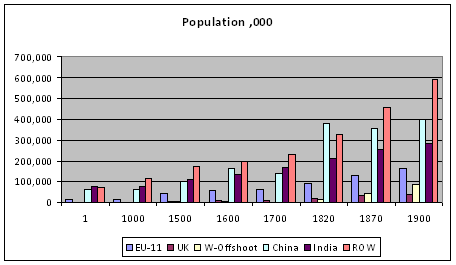
\includegraphics[width=0.9\textwidth]{C:/Users/Steve/Desktop/VAT/Projects/Research/publish/empire.barking/images/pop.png}
%\end{figure}

\begin{figure}[h!]
\center
\caption{Global population levels, source: Angus Maddison \citep{maddison_world_2007}}
\label{fig:popLevel}
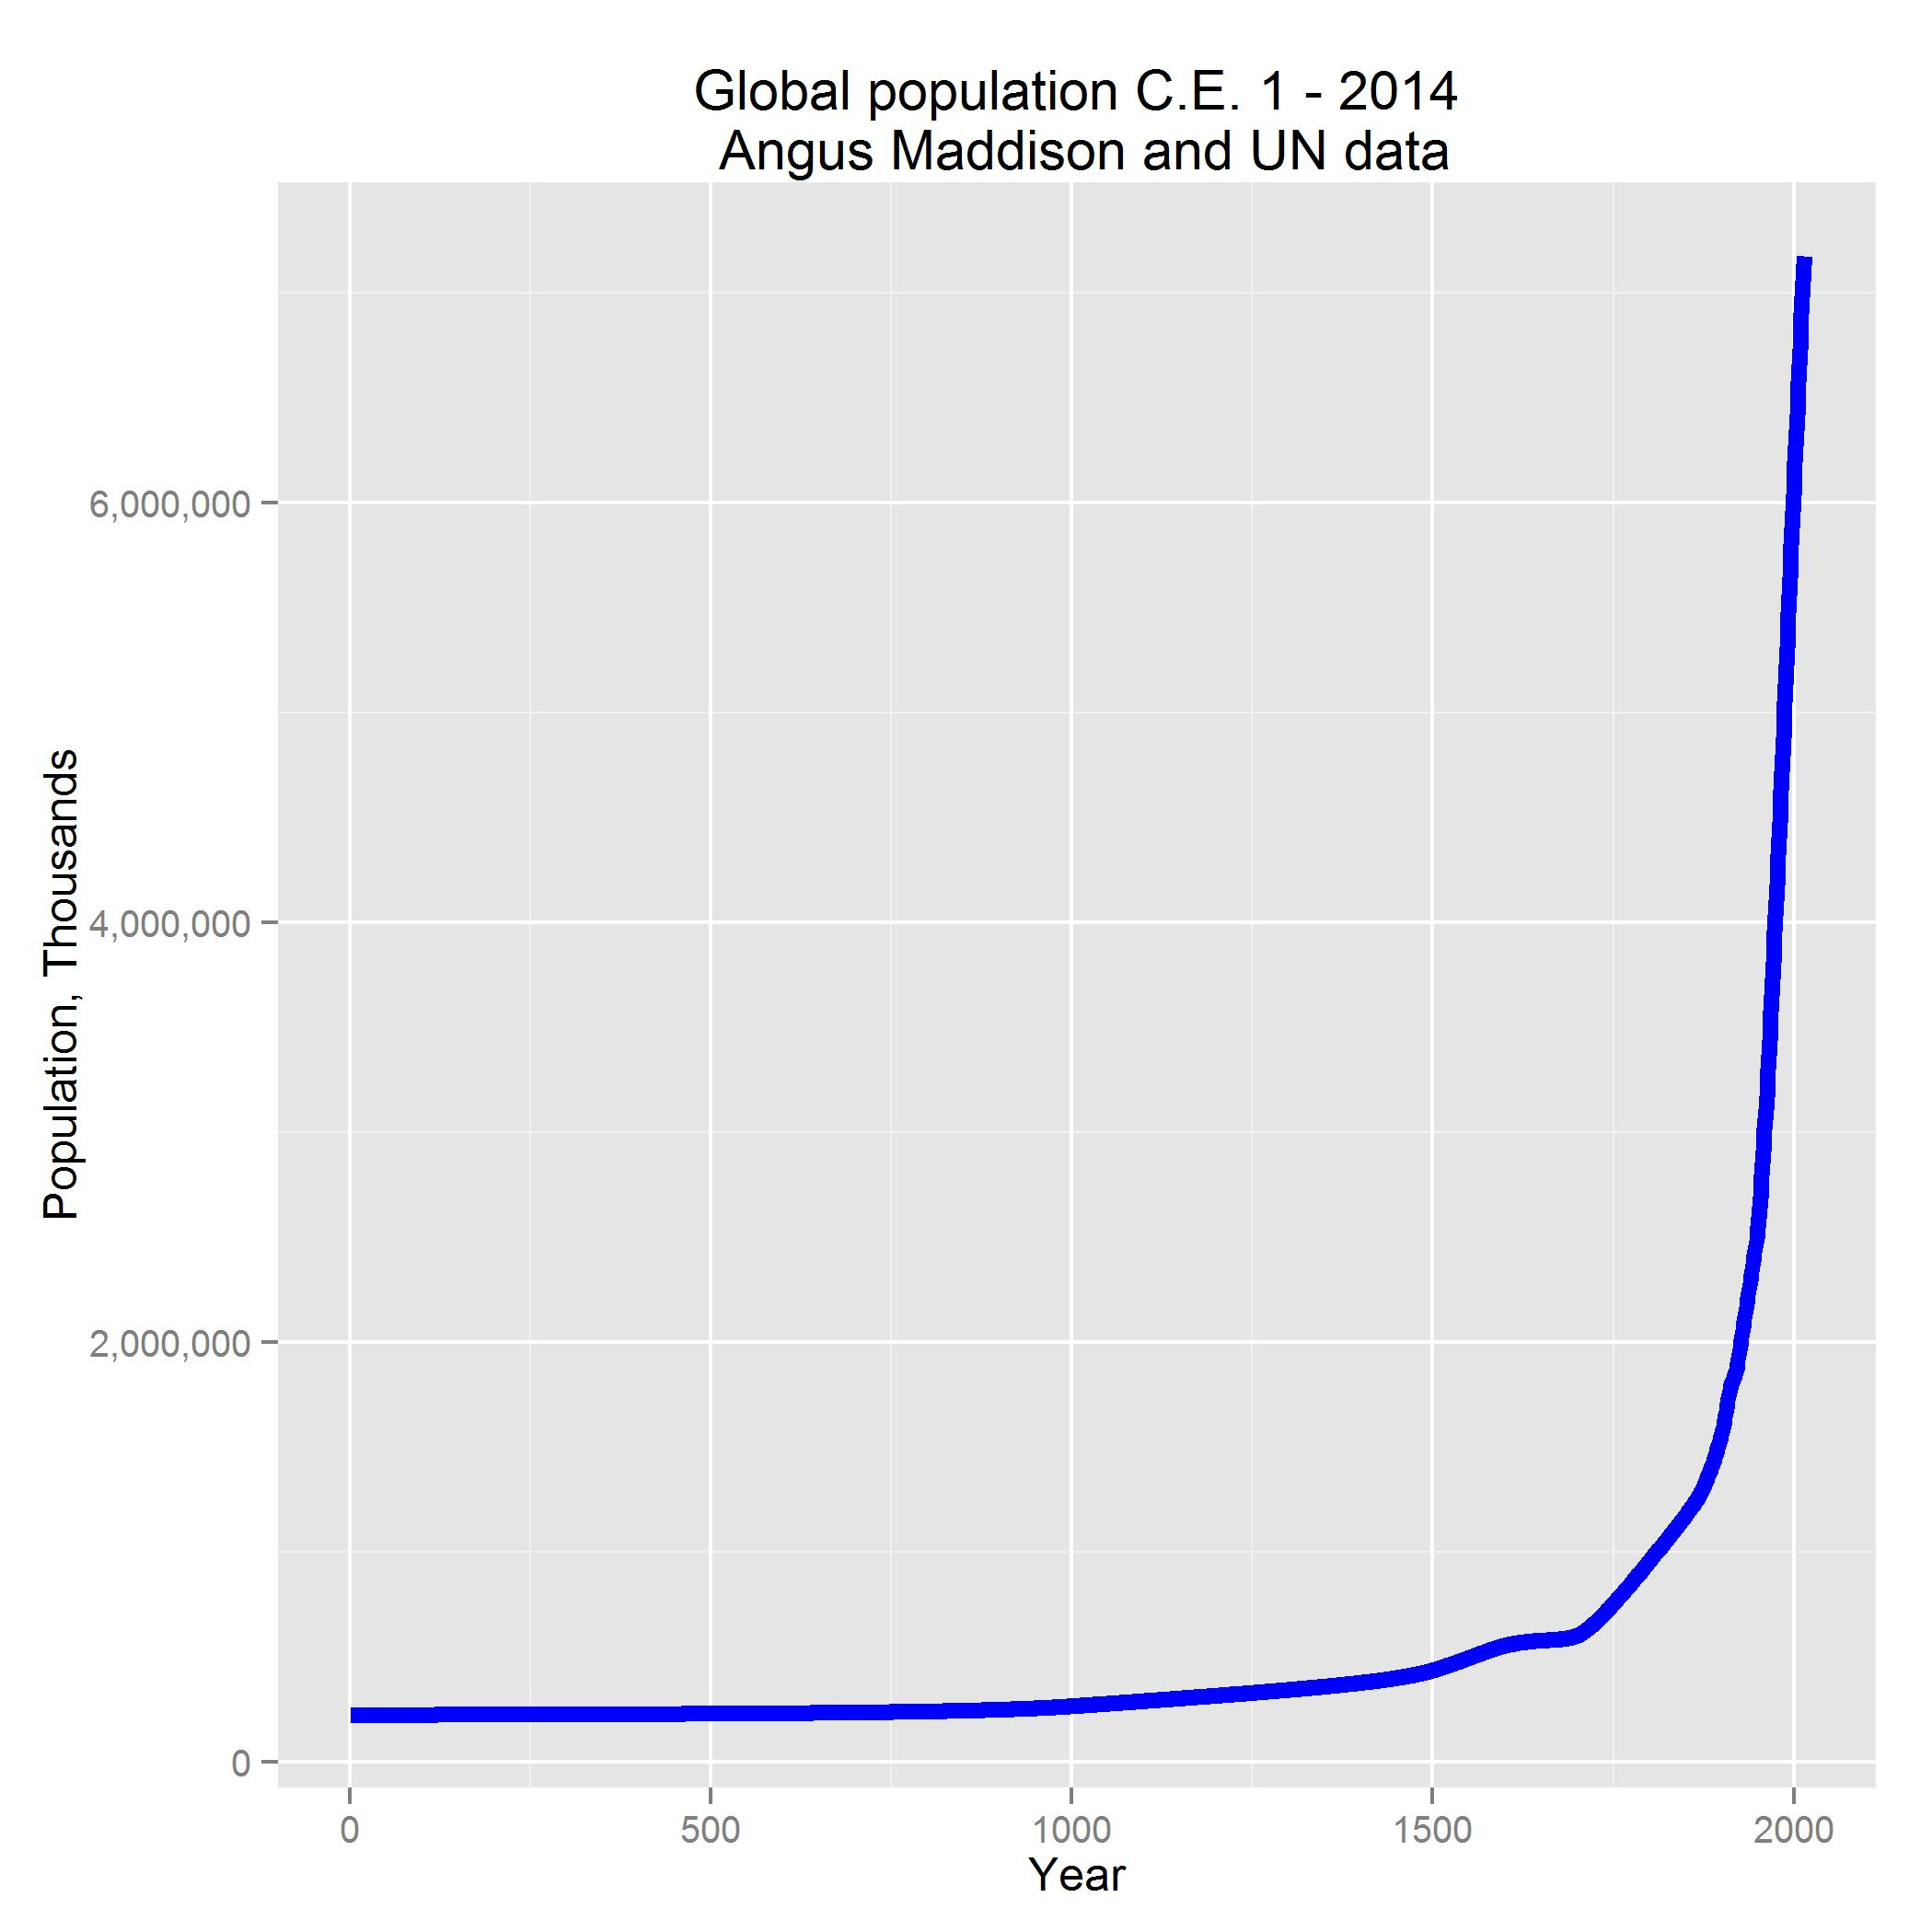
\includegraphics[width=0.9\textwidth]{../images/pop1-2014.jpg}
\end{figure}

%While England's population is imperceptible at this scale until after 1500, western Europe is growing significantly, and all these regions are increasingly part of England's trading area. 

One can clearly see the goblal population liftoff in the late middle ages, accelerating during the early modern period, and ``going exponential'' during the EIR. England's population growth follows this pattern. I claim that population growth essentially everywhere in the world is sufficient to account for the demand expansion that the commercial expansion, first in the Dutch Republic then England, required in order to bloom. I note that perceptible per-capita gains to total output do not happen until after 1500 in Western Europe, and the great gains in living standards await the second-phase EIR in the nineteenth century. Now that we have a sufficient story for ever-increasing demand, we can return to the supply side which limited growth in a pre-EIR world.

Mantoux analyzes land redistribution in England, focusing on the enclosure movement. This episode is fascinating and important in that it freed agricultural labor to urbanize and fuel the EIR and, as a by-product, raised agricultural productivity. While not central to my story here, I believe I can, in future work, make a claim that it was early industrialization in the woollen industry that motivated the enclosure movement. For now, we move on.

Mantoux traces the beginnings of machinery in the textile industry and the role of capitalist undertakings resulting in the rise of the factor system. He discusses the technologies, such as the knitting frame and the silk throwing mill, and their inventors in detail. This includes a fascinating narrative on the transition from tools to machines that changed the nature of labor, described as essentially a skill transfer from man to machine, that initially used wind and water power but enabled the application of steam-power when that was feasible \citep[p.189-191]{mantoux_industrial_1961}.

He relates the canonical story of John Lombe pirating Italian silk-throwing technology and using it to build a very large (five hundred feet long and five or six stories high) Derwent factory that was centrally powered by a water wheel. This was in about 1718, and illustrates the three key points: the skill transfer from men to machine, the power transfer from men or animals to something much more scalable, and the demand for capital to realize this achievement. John's brother Thomas supplied that capital; the capital source is likely from Thomas' merchant activities. The factory employed about three hundred workers \citep[p.191]{mantoux_industrial_1961}. 

This clearly was the prototype for the future of the factory system in cotton and woollen textiles and thus heralded the course of the EIR over the following 150 years. The more famous inventors/entrepreneurs, John Kay (fly shuttle), John Wyatt (cotton spinning machine), William Hargreave (spinning jenny), Richard Arkwright (water frame), and so many others, built on this successful factory template, built the EIR, and greatly increased the demand for capital.

The factory system was a fertile ground for the application of steam-power; this loosed the constraints of finding a suitable water-power location, or unreliable wind power source, and thus began the essentially uninterrupted productivity rise leading to ever-increasing per-capita living standards. This also led to the revolution in land transportation represented by the railroads, and the maritime transport revolution of the steam ship. And, naturally, led to a great increase in the demand for capital.

While aggregate capital stock data seems somewhat sparse for the era, a simple illustration will show the growth-rate leverage capital had as growing population demands drove aggregate output.

A 1984 Journal of Economic History article by Jeffrey G. Williamson, ``Why Was British Growth So Slow During the Industrial Revolution?'', provides a survey of capital growth rates and, importantly, estimates through time of the Capital/Output ratio. Williamson draws on work by Phyllis Deane, Floud and McCloskey, and Simon Kuznets. I partially reproduce his table \citep[p.701]{williamson_why_1984} as table \ref{tbl:y/k}:

		\begin{table}[h!]
		\centering
		\caption{British capital productivity. Source: Jeffrey Williamson \citep[p.702]{williamson_why_1984}}\label{tbl:y/k}
		\begin{tabular}{lrr}
		\toprule \hline
		Period&Capital's productivity Y/K&Calculated K/Y\\
		\toprule
		1761--1820&0.36&2.78\\
		1791--1820&0.38&2.63\\
		1821--1860&0.53&1.89\\
		\bottomrule
		\end{tabular}
		\end{table}
		
So before 1820, for every additional British pound of aggregate output, more than 2.6 British pound's worth of capital stock was required. I will not here recount the growth in Gross Domestic Product estimates for that period except to summarize this is the period that GDP growth rates went exponential in Britain. I note that while growth rates of GDP and capital will be the same, the capital growth rate operates on a large base such that capital accumulation is increased at the multiplied rate.

It does not appear either from Nef or Mantoux that capital supply was a real constraint, with investment flowing from wealthy merchant capitalists, wealthy landowners (often nobility), and eventually a banking system. Instead, capital supply appears to have been called forth by capital demanded to keep up with aggregate demand growth and the technical productivity factors summarized by the K/Y ratios in the table.

Thus we have a straightforward supply and demand economic story for the rise of industrial capitalism. This was facilitated by the fact that capital stock is consumed only over many units of output, thus the relative mathematical ease of building large capital accumulations during the nineteenth century.

%% insert here the role of tangible capital as an energy conversion machine ala Cottrell %% 1/6/15
\section{The primary roles of capital in the EIR}
Tangible capital has two primary roles in the EIR:

The first is the infrastructure investment required to extract and transport coal as a fossil energy source used initially to substitute for ever more expensive wood-supplied Joules in heat-using applications. Increasing demand caused deforestation, causing rising wood prices. Compared to using wood as the primary heat source, English coal supplies were distant, deep, wet, but ultimately cheaper than wood. As John Nef documents \citep{nef_rise_1932}, the investment required for successful coal extraction and distribution was large and historically unprecedented.
 
The second is to replace muscle-supplied power inputs to the production process with steam-powered mechanical devices. The energy input is largely from coal during this revolution, so the tangible capital devices use fossil inputs to provide power in the form of, typically, rotating or reciprocating motion through the mechanical application of steam -- the steam engine. 

There is an important class of mechanical devices -- gears and levers, say -- which amplify muscle power by allowing increased muscle power input for a given output, allowing low-intensity muscle power to leverage up their power inputs to accomplish higher-intensity tasks. Note that this requires added muscle Joule inputs for a given amount of output, recognizing humans have fixed potential power output per unit of time; this is not the kind of capital device I focus on here which allow essentially unconstrained power inputs per unit of time. Such pure mechanical muscle assists are not the important technologies in the second phase industrial revolution. 

As I cite in this article, Paul Mantoux describes this revolution in great detail, using the steam-powered mechanization of both the English woollen and cotton textile industries as primary examples \citep{mantoux_industrial_1961}.

%%describe the attempts at water and wind power (check Temin and Romans)
There were non-coal non-muscle power inputs to manufacturing through much of recent history. These were either water- or wind-powered rotary machines and were precursors to steam-powered machines. In recent scholarship, \"{O}rjan Wikander claims ``Today, we may state with confidence that the breakthrough of the water-powered mill did not take place \ldots in the early middle ages, but rather \ldots in the first century A.D., or perhaps even slightly earlier.'' The water wheel was known and used during the late Roman republic or the early empire (as cited in \cite[p.224]{temin_roman_2012}). Of course, the Arkwright water frame was an EIR water-powered mechanical cotton spinning device, but the true energy revolution started when the essentially unconstrained scale of steam power was applied through such devices to manufacturing processes.

Note that in my theory of industrial revolutions (formalized here \ref{eq:mrp} ) capital is always labour substituting since, while the Joules of energy which are inputs to production are either muscle or fossil inputs but, for each Joule, not both, tangible capital applies fossil Joules to industrial processes. They are mutually exclusive. Of course, both organic and inorganic energy input sources for a production process can be mixed, and it is this frequent case that causes the ``complements'' versus ``substitutes'' confusion.

%% should I use cottrell - I think yes to underline the starkness of the input choice
To crystallize the starkness the energy revolution represented in choosing among energy input sources, I summarize briefly from Fred Cottrell, who wrote ``Energy and Society'' in the mid-twentieth century: Cottrell sharply contrasts low-intensity and high-intensity energy regimes and societies. Low intensity ``converters'' include human and animal power using plant-based input sources, and water- and wind-mills \citep{cottrell_energy_1955}.

The first high-intensity converter in Cottrell's history is the sailing ship, which provided at least an order of magnitude increase in energy surplus over low-intensity converters, and dramatically changed the economics and institutions of the world's economies.

Cottrell then continues to recognize that the most disruptive high-intensity converter was the steam engine, the signal technology of the EIR. The steam engine disrupted the economic systems and, thus, their social systems and institutions, a legacy of turmoil that continues to this day.
%% wilson article on roman power

\section{Summarizing the story}

First-stage energy revolutions, the transition from wood to coal for heat-consuming industries and households, require substantial capital to (invent and) build extraction, transportation, and production infrastructures. Before this, there was likely no large-scale demand for capital or, from a different point of view, the industrial scale made possible by industrial capitalism was not required to meet market needs. This type of energy revolution occurred at least in China during the Sung dynasty (ninth-, tenth-, and eleventh-centuries), and in early-modern England.

England built their second-stage energy revolution on their first-stage infrastructure, using a mechanized factory system converted to steam power to dramatically increase labor productivity. China did not. Until the modern era, this was the only known complete industrial revolution, was accompanied by greater demand for capital, and led directly to the institution we now call industrial capitalism.

This paper seeks to identify a prime-mover in the explanation of what is a very complex social system, industrial capitalism. Following the suggestions of Historical Materialism and endogenous institutional theory that depend on economic causes, the seminal change in demand for capital was the energy revolution that required replacing increasingly scarce and expensive wood with more capital-intensive coal for heating, and then, with ever more sophisticated technology, replacing labor power with coal power. Thus, I suggest these energy revolutions are the prime-mover in the rise of industrial capitalism.

\section{Brief conjectures on the future of demand for capital}

The coal and steam revolutions required large investments in centralized structures and infrastructures. Current energy extraction, processing, generation, and transportation investments remain large and highly centralized. Should a future energy revolution result in highly distributed and very inexpensive energy sources, the need for large capital investments will be diminished. The author believes these radical energy technologies are in train; that discussion should remain outside this paper.

The factory system added to the demand for capital with large centralized automated manufacturing dominating the nineteenth and twentieth centuries; global supply chains have somewhat distributed manufacturing infrastructures, but they remain capital intensive. We are living through the very beginning of a revolution in manufacturing, 3D printing, that holds the promise of a highly distributed, even consumer based, manufacturing system that will be much less capital-intensive.

These possible trends will be enhanced by a likely peaking of global population in this century; the driver of the original EIR will therefore be removed. Total output will fall.

I illustrate this in figure \ref{fig:popLogDiff}. This transformation of the population levels shown in figure \ref{fig:popLevel} displays the change in the annual population growth rates. For my argument here, there are two noteworthy features:
\begin{itemize}
\item Until about 1960 and dating to, likely, at least the beginning of the Neolithic Era, population growth rates had a positive second derivative, so always increasing growth rates to levels above two percent per year at the peak. This, under my theory, implies ever-increasing demand for capital.
\item 
Since about 1960 that trend has (strongly) reversed, and we note since then that population growth rates have a negative second derivative. While the first derivative is still positive (population levels are still increasing), this reversal will have profound consequences. For my current argument the implication is that global aggregate demand will eventually peak, then decline. Under my theory of industrial capitalism, demand for capital must then also decline.
\end{itemize}

\begin{figure}[h!]
\center
\caption{Global population growth rates, log differences}
\label{fig:popLogDiff}
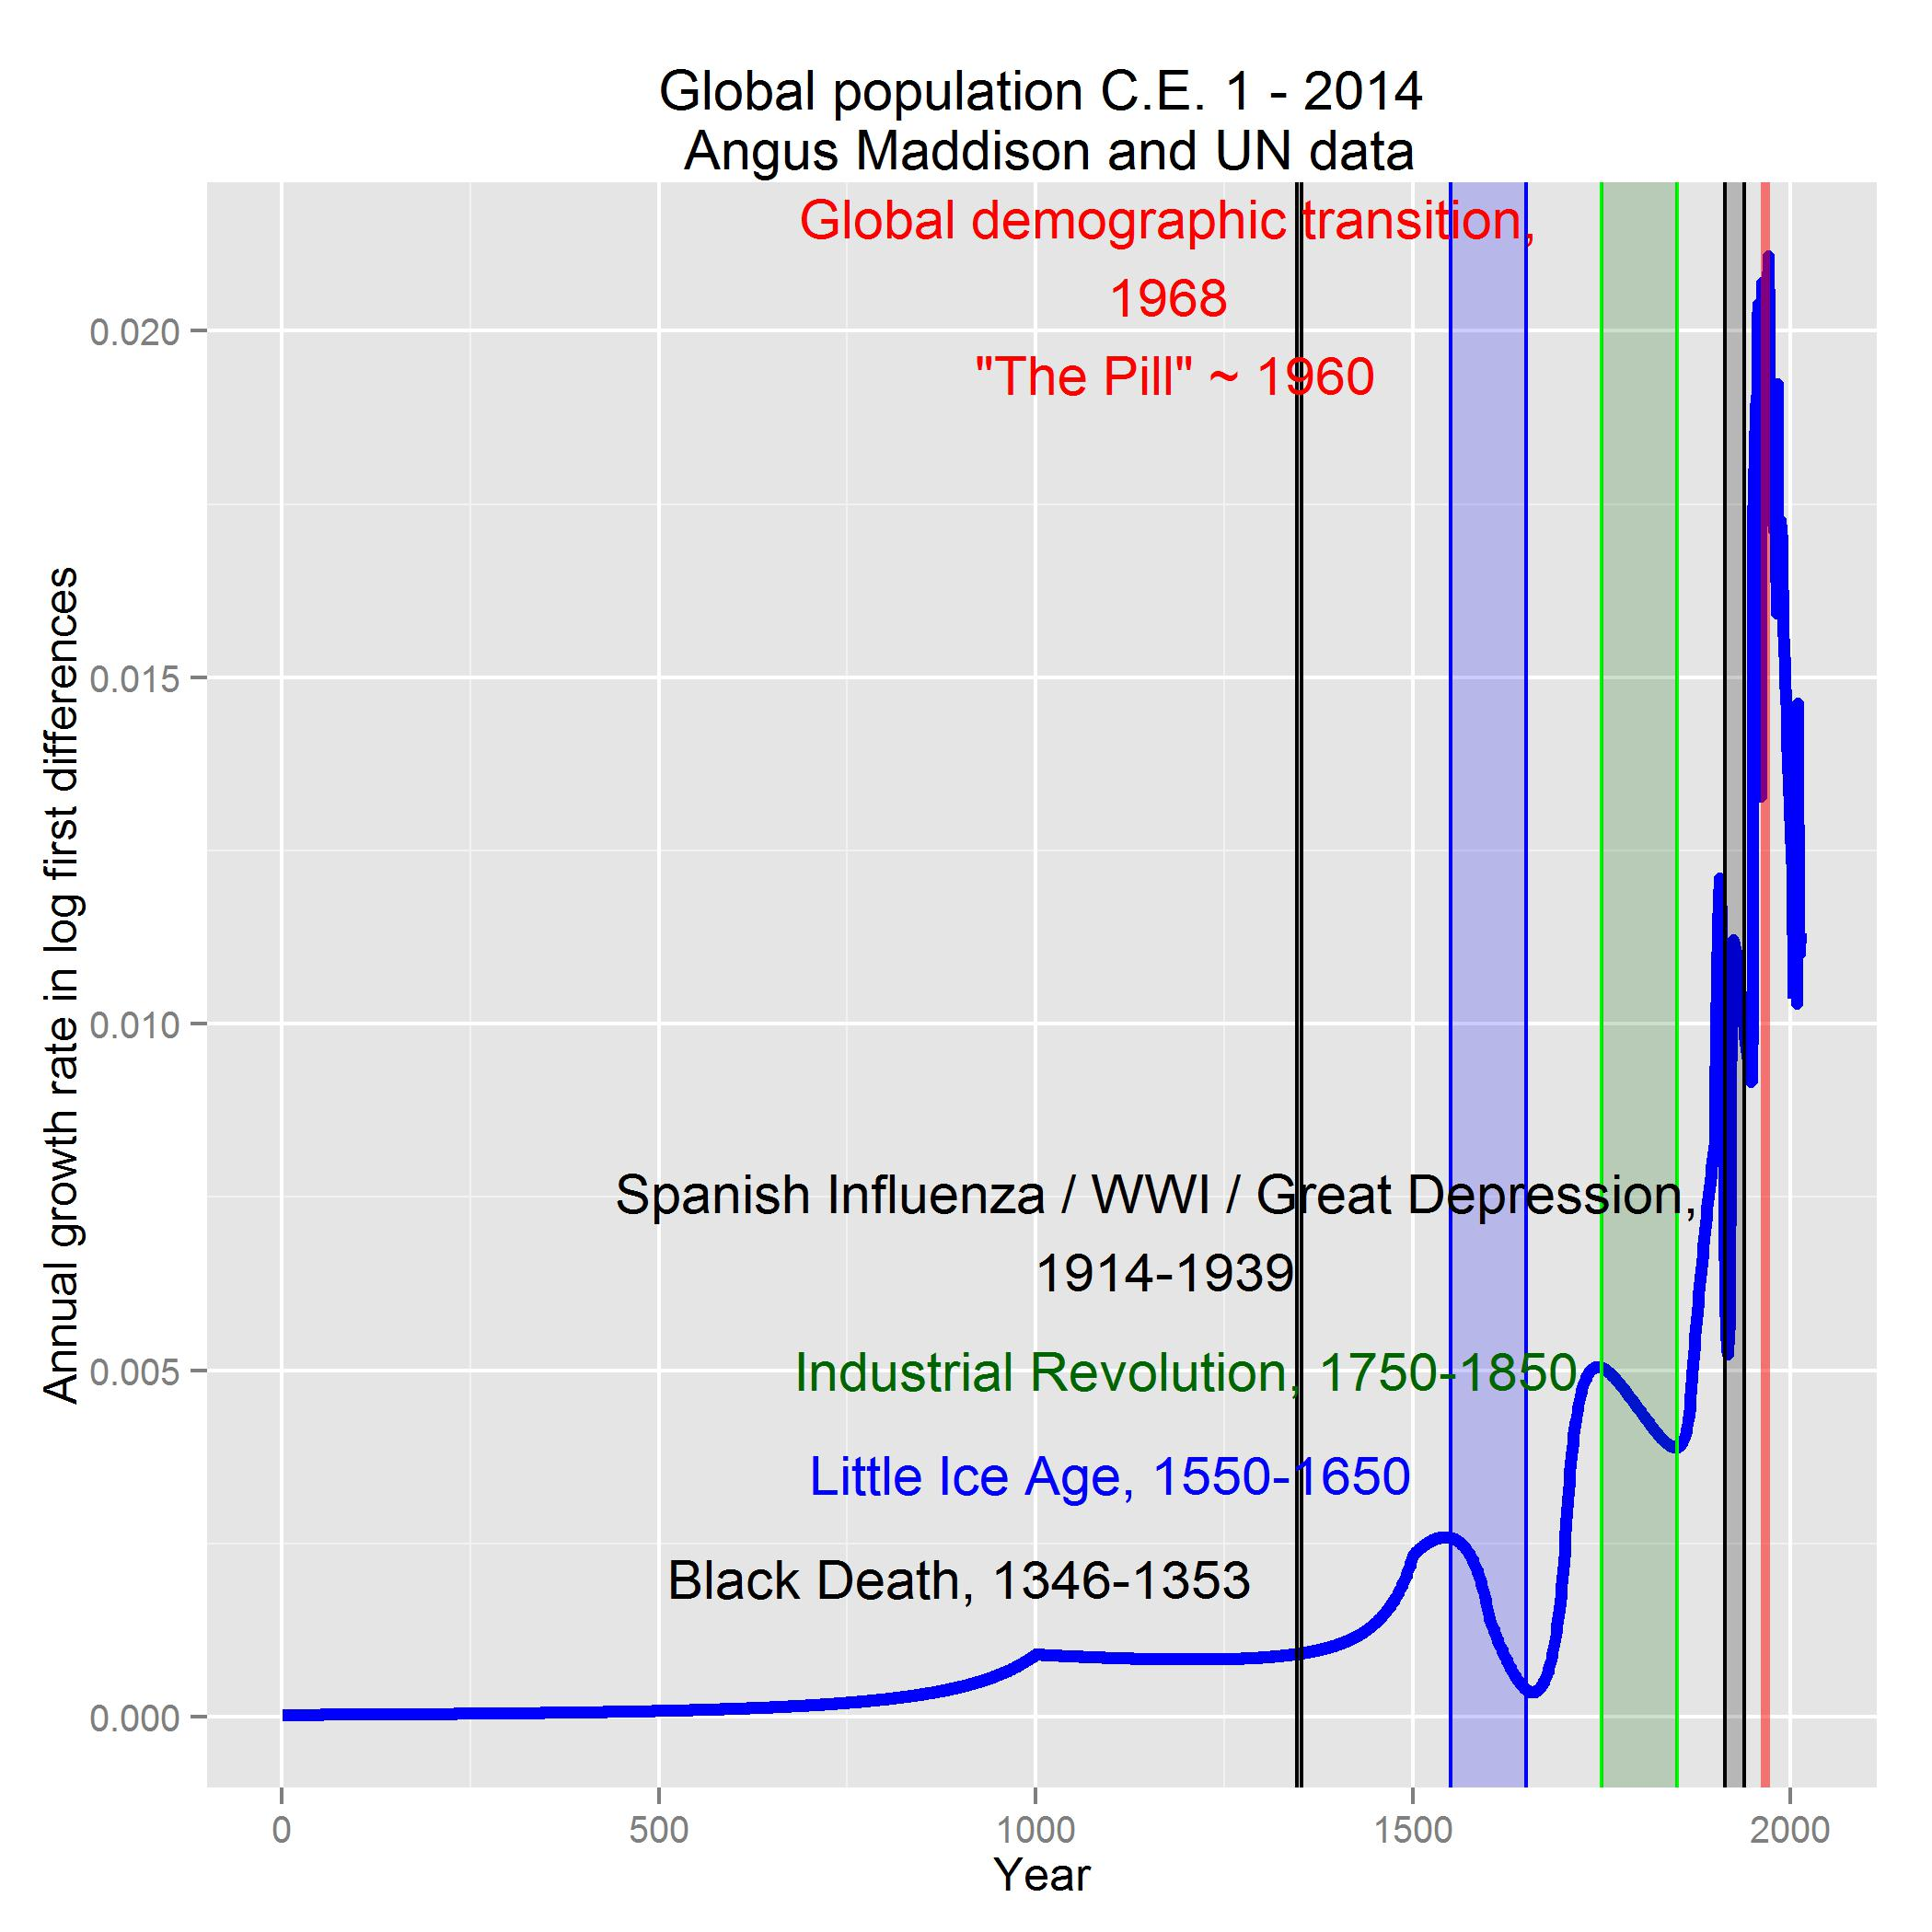
\includegraphics[width=0.9\textwidth]{../images/logDiffPop1-2014.jpg}
\end{figure}

Whether these trends will be sufficient to diminish the rentier power of industrial capitalism remains to be seen, but at the very least this is an intriguing possibility. If the demand shrinks, so will the supply, and thus the accumulated power of capitalists can begin to fade.

\section{Institutional postscript}

Some may wonder, even fret, that I do not depend on the various pieces of New Institutional Economics to help explain this story. It is my strong belief that the institutions of NIE are largely endogenous to more fundamental economic changes. This does not mean they are not supportive of innovation that occurs after the real inventions. Indeed, the only ``institution'' I need to tell my story is a market economy. These have existed for a very long time. Rising population causing demand, deforestation causing coal substitution, and high English wages causing steam-power substitution are, I hope I have convinced the reader, sufficient to explain the EIR and the rise of industrial capitalism and all the institutional changes that it caused.

Further, my thesis does not negate the many valuable institutional analyses and insights of radical political economists; I simply want to understand causality for its potential to suggest the future.

\newpage
\section{Technical Appendix}
\label{sec:techAppendix}

\subsection{Importance of energy for growth and development}
\begin{table}[h!]
\begin{center}
\begin{tabular}{lr}
\hline
Period&Pearson Correlation Coefficient: \\
&energy and GDP\\
\hline \hline
England 1300-1873&0.998\\
World 1980-2008& 0.993\\
\end{tabular}
\caption{Energy/GDP correlations -- the case for energy revolutions}\label{tbl:cor}
\end{center}
\end{table}
%\newpage
\subsection{Cross-country history of energy consumption}
\begin{table}[h!]
	\centering
	\begin{tabular}{lrrrr}
	\hline
	Year&England&China&Netherlands&India\\
	\hline \hline
	1650$^a$&&&0.63&  \\
	1820&0.61&&&\\
	1840$^a$ &&&0.33& \\
	1870&2.21&\\
	1970$^a$ &&&8.07&0.33 \\
	1973&&0.48&&\\
	1998$^b$&6.56&1.18\\
	2008$^b$&5.99&2.56&9.86&  \\
	\hline
	\end{tabular}
	\caption{Per-Capita Primary Energy Consumption,	annual Tonnes of Oil Equivalent. \textit{Source:} Angus Maddison, $^a$de Zeeuw, $^b$US DOE EIA}
	\label{tab:capitaEnergy}

	\end{table}
\newpage

	\subsection{Theory of industrial revolutions}	
		\begin{equation}
		\label{eq:mrp}
		\frac{\text{Marginal Product}_{\text{wood Joule}}}{\text{Price}_{\text{wood Joule}}} \ll \frac{\text{Marginal Product}_{\text{coal Joule}}}{\text{Price}_{\text{coal Joule}}}
		\end{equation}
		\vspace*{-0.2in}
		\begin{center} First-stage energy revolution: China 900 -- 1200 (Northern Sung);\\ England 1590 -- 1700
		\vspace*{0.2in}
		\begin{equation}
		\label{eq:mrp2}
		\frac{\text{Marginal Product}_{\text{labor Joule}}}{\text{Price}_{\text{labor Joule}}} \ll \frac{\text{Marginal Product}_{\text{steam Joule}}}{\text{Price}_{\text{steam Joule}}}
		\end{equation}
		\vspace*{-0.2in}
%		\begin{center} 
		Second-stage energy revolution: England 1700 -- 1873, but not in China\\
		\vspace*{0.2in}
		\end{center}
		
		The RHS of (2) was so large that it induced a major positive aggregate supply shock, the EIR, and large income effects.
		
		This is intended to be didactic, not ideological, that is not supporting marginalism in general. Note that replacing neo-classical marginal pricing with more general average pricing or prices of production will not change this theory.

\section{References}
		\bibliographystyle{plainnat}	
	\bibliography{diss3}



\end{document}

%\section{Variations on the story}
\section{Research question} %1
I seek to identify empirically, economically, and eventually institutionally, what facts constituted the English Industrial Revolution. What was it, why did it occur, why did it happen when it did, why did it happen in England and only England? This paper addresses a subset of this agenda, describing what happened empirically, and suggesting the economic events that caused this result.
\section{Hypotheses}
The English Industrial Revolution (henceforth EIR) was the first example of modern economic growth.\footnote{Kuznets 1996} There were both macroeconomic and microeconomic forces that were causal. The primary driver of the EIR was an energy consumption revolution. There is limited statistical space for a very few causal institutional or cultural events.	%2

\section{Research approach}
As this is a largely data-driven project, I first describe the data sources and comment on their limitations.

\subsection{Data}
Table \ref{tbl:dataSources} enumerates the primary data sources in this paper.
Figure \ref{fig:overall levels} displays the three data series keyed to the sources.

\begin{center}
Table \ref{tbl:dataSources} about here
\end{center}

The energy consumption data from Roger Fouquet covers England and Wales for the entire study period (1300 -- 1873). A word about why I end analysis in 1873: that is the end date Robert Allen \footnote{Allen (2009)} places on the EIR. I can make a case from the data that it was a few years later, perhaps 1876, but there is little difference.

The gross domestic product data is composed from data series from Graeme Snooks and Lawrence Officer. The normalizing index is 2005 Great Britain Pounds. For this study period, those were the closest to England/Wales gross domestic product data that I have found.

The population data is composed from data series from Graham Snooks and Mitchell. For this study period, these were the closest to England/Wales population data I have found. Figure \ref{fig:overall levels} summarizes the data series by author/time-span.

\begin{center}
Figure \ref{fig:overall levels} about here
\end{center}

All such historical series are clearly composed, modelled, estimated, and thus fraught; a common problem with macroeconomic data to the present day. That said, I reserve special admiration in general for the work of the English economics historians. And these series are generally bounded by their starting point, their ending point, and various benchmarks along the way. The historians use a variety of methods to validate their work. In general, they cannot be too far wrong with the worst case being shifts by several decades in the shape of the curve. And the later data is generally better.

I do not claim these series are definitive for all time, simply the best I know of at this point, and probably good enough. Their shapes clearly affect the analysis to follow. As better series appear, I will incorporate them into this analytic framework.


compare gdp, energy, pop series. table for sources\\
pop -- maddison vs. my current splice\\
gdp -- maddiosn vs. ?\\
e -- foquet vs. warde


\subsection{Methodology}		%3
This paper uses largely descriptive statistics of the three data series to describe the EIR. Much of the discussion of results depends on the graphs. I do provide analytic statistics including correlations, sample tests, structural break analyses, bi-variate Granger causality tests, \footnote{Granger (1969)} and a scatterplot of energy consumption and gross domestic product. I also discuss the results in the context of microeconomic and macroeconomic theory.

I do not estimate a formal empirical model, such as a regression, as that seems redundant after examining the scatterplot. The correlation between energy consumption and gross domestic products is strikingly, and visibly, strong.

In an appendix, I do provide substantial time series analyses as a foundation for formal modelling when this work is extended to examining how important certain historical events are in explaining the outcome. I believe that will be the best use of formal modelling; the approach in this paper is sufficient to support my stated hypothesis.

\section{Results and discussion}		%6

\subsection{Modern economic growth}
Simon Kuznets defined modern economic growth as high rates of growth of per capita product and population. Figures \ref{fig:ggdp} and \ref{fig:gdpLog} indicate that England experienced high rates of growth of per capita product in (possibly) two eras, from 1500 to 1600 that was not sustained, and after 1750 that was mostly sustained. Clearly after about 1820 England had a high and sustained rate of growth in per-capita product here measured as gross domestic product. The annual rate after 1800 was 2.4 percent per-year total growth and 1.1 percent per-capita growth as seen in table \ref{tbl:growthByCentury}. Figure \ref{fig:popLog} shows the log of population growth which, supporting the Kuznets definition, mirrors GDP growth with a lag.

\begin{center}
Figures \ref{fig:ggdp} and \ref{fig:gdpLog} about here\\
Figure \ref{fig:popLog} about here\\
Table \ref{tbl:growthByCentury} about here
\end{center}



\subsection{An energy revolution}
This paper's central assertion is that the EIR was, primarily, an energy revolution. Specifically a consumer consumption revolution supported by an energy supply revolution. To support that hypothesis, first I present the data:

Figure \ref{fig:energyLog} displays the log of energy consumption over the study period; the vertical lines are formally determined structural breaks. The log presentation enhances rate-of-change and potential structural differences in the series. I note four significantly different periods or regimes. The first is from 1300 to 1500, a period dominated by the Black Death epidemic; energy consumption clearly drops, then recovers. The second is from 1500 to roughly 1600 as determined by the structural break. The third is the period from 1600 to roughly 1750; note that the rate-of-change of energy growth in this period is approximately the same as in the prior period; this rate of change similarity is confirmed by the presentation in table \ref{tbl:growthByCentury}. The final period is from 1750 through 1873; clearly the energy consumption rate-of-change accelerates as confirmed by the structural breaks in \ref{fig:energyLog} and table \ref{tbl:growthByCentury}.

Based on the structural changes, and based on the hypothesis that the EIR was an energy revolution, I propose that the revolution happened in two stages: one starting in the late sixteenth century, and one starting after 1750. The first, under this hypothesis, would have set the stage for the second.

\begin{center}
Figure \ref{fig:energyLog} about here
\end{center}

If we were to overlay the energy levels or logs charts with the GDP levels or logs charts the similarities would be striking; I think a more productive view is figure \ref{fig:energyVsGdp}. This figure shows levels of energy consumption through the study period, and has a standardized series of GDP for the same period. By standardized I mean matched in levels at the first period; the series' evolutions thus show differences in growth rates through continuous time. Again we see four distinct regimes. The most notable features are the period of 1500 to 1600 when growth in GDP clearly leads energy growth, and after 1750 (especially after 1800), when energy growth leads GDP growth.

\begin{center}
Figure \ref{fig:energyVsGdp} about here
\end{center}

The dynamics of GDP growth and energy consumption growth can be seen more clearly by taking the differences of the last graph.

\begin{center}
Figure \ref{fig:energyVsGdpDiff} about here
\end{center}

The Black Death and its aftermath affected the relatively flat net economic performance from 1300 to 1500, but set the stage for a growth boom in the period 1500 to 1600. In the period 1600 to 1750 growth in both relatively flattened, and then boomed during the period 1750 to 1873.

\subsection{Correlations}

Next, I present some simple analytic statistics to support the hypothesis that the EIR was at its root an energy revolution responding to a positive demand shock.

Starting simply, a Pearson's correlation coefficient and a paired t-test of energy consumption and GDP yields the results in table \ref{tbl:fitTest}: 

\begin{center}
Table \ref{tbl:fitTest} about here
\end{center}

These simple results suggest that the two series are statistically very similar; a more formal co-integration test could be expected to be positive and is presented in section \ref{app:Appendix B}. However, for the purposes of this paper, a scatterplot of the series is shown in figure \ref{fig:scatterplot}. The solid green line is a linear fit; the solid red line is a \textit{lowess} (non-parametric, non-linear) fit.

\begin{center}
Figure \ref{fig:scatterplot} about here
\end{center}

Clearly, there is a very high correlation between the two series. For current purposes, more formal modelling is not needed. Overall statistically, these two series are very close to being the same, that is they share a common data generating process. In a strong sense this is a validation of the thermodynamic view of economic production and growth at least in the long run.

However, this overall view does hide important dynamics that the data contain. I examine these more subtle results next, and thereby set the stage for telling a history of the EIR.


\subsection{Causality tests}
I continue by using basic statistical causality tests, specifically the Granger bi-variate test to examine changing dynamics. \footnote{Granger (1969)} Table \ref{tbl:grangerEnergyGdp} reports this result for the four main eras already identified.

\begin{center}
Table \ref{tbl:grangerEnergyGdp} about here
\end{center}

During the first energy/GDP era Granger causality between energy and GDP runs both ways at significant levels; while not ignoring these results, I do not want to over-interpret what was happening given the huge shocks of the Black Death. However, it is significant for later eras that the Black Death caused wages to rise, and the European Marriage Pattern (EMP) \footnote{Hajnal (1965)} increased family incomes entering the early modern period.

During the second energy/GDP era of 1500 to 1600 causality from GDP growth to energy consumption is weakly significant; energy Granger-causing GDP growth is not at all significant.

In the third energy/GDP era of 1600 to 1750, neither direction of causality is significant. This will turn out to have important implications as I build the historical shortly for the EIR.

In the fourth energy/GDP era of 1750 to 1873, we again see both directions of causality significant, with GDP Granger-causing energy consumption being the stronger.

Notably, through the entire study period GDP Granger-causes energy consumption more significantly than energy Granger-causes GDP, but causality is significant in both directions.

\subsection{Structural breaks}

Figure \ref{fig:structural} juxtaposes frames with logs of energy consumption, gross domestic product, and population, each with formal structural break lines noted. The point here is to note the correspondence of the structural breaks, again suggesting the same underlying data generating process.

\begin{center}
Figure \ref{fig:structural} about here
\end{center}


\section{Discussion of results}

I can now present a story of the EIR as supported by the data presented above. 

\subsection{Narrative discussion}

Energy/GDP era one, due to the Black Death, saw both negative demand and supply shocks, but set the stage for the following EIR eras. 

In energy/GDP era two, wages rose due to the negative labor supply shock of era one. Demand had positive shocks, as a result both of wages and  of incomes rising due to later marriages and women working -- the EMP outcomes. Supply expanded as can be seen by the stronger growth of energy consumption. Refer to table \ref{tbl:growthByCentury} or figure \ref{fig:energyLog}. This era provided the demand shocks and supply constraints that caused the EIR. It started here.

In energy/GDP era three, rates of growth for both GDP and energy consumptions stagnated. A story that fits the data, and the history, is that this era was one of a negative energy supply shock, and for the whole economic system growth slowed. This era was the transition between primarily wood-supplied energy to primarily coal-supplied energy. As London grew because of exports and world trade domination, wood became scarcer and more expensive, driving demand for coal for heating from the north east. You can see this pattern during the 1600 to 1750 era three in the following figure \ref{fig:woodCoal}.

\begin{center}
Figure \ref{fig:woodCoal} about here
\end{center}

This demand for heating coal and the fortuitous geology of the English coal mines created the path necessary to support energy/GDP era four, in which the EIR accelerated into modern economic growth via the virtuous, mutually reinforcing, growth cycle between GDP and energy consumption. 

The geology story is that the coal mines were water-infused, and as they were dug deeper, more water had to be pumped out. This provided an economically feasible site for the seminal but very inefficient Newcomen steam engines to pump the water. The coal was essentially free to power the engines. Human or horse power were too expensive. And as the steam engines gained efficiency, they began to be applied to industrial capitalism. That is the story of energy/GDP era four, the age of steam. I turn next to telling that story in more detail; again it is an economic story, supported by data.


\subsection{Theory discussion}

We have already examined the GDP and energy consumption data for the fourth era. To finish the story, I will retreat to economic theory. First, I summarize the eras in aggregate supply/aggregate demand charts; second, I address the question of what were the incentives for the English inventor/entrepreneur to spend the time and money to make the inventions of the EIR, particularly the steam engine. To do this, I appeal to microeconomic theory.

Figure \ref{fig:asad} displays the four eras in an aggregate demand/aggregate supply (AS/AD) framework. The dotted lines indicate prior locations of AS/AD; solid lines indicate the ending locations. Lines colored red indicate the constraint in each era. These are obviously abstract depictions of the history I have told above. I do this for two reasons; first to solidify and emphasize the history so that the debate can commence; second to provide a framework for later projects incorporating the institutional and cultural events into the history. If we can agree on the AS/AD by era, then we can hypothesize about those events that might have caused the location or shape to change and then test those ideas in an econometric framework.


\begin{center}
Figure \ref{fig:asad} about here
\end{center}

A notable observations is that energy/GDP era four is the first in which supply was not the constraint; according to the Granger causality tests, supply and demand were jointly constraining in that era, but the lack of relative barriers in consuming energy was surely the defining event of the era.

Second for the theoretical discussion of the EIR, it is important to consider at the microeconomic level what can explain the event. At this level I will discuss only the supply side having already suggested the demand side factors. So the question becomes what were the incentives or motivations of the English inventors and entrepreneurs during energy/GDP eras two and three, so from 1500 through 1750.

For this analysis I rely on three sources; first the contemporaneous comments of a key participant in the EIR; second the excellent work of Robert Allen; and third an appeal to microeconomic theory.

Jean Theophilus Desagulier had a large influence on the EIR. He was an eighteenth century English ``natural philosophe (physicist), member of the Royal Society, colleague of Sir Isaac Newton, and author of ``A Course of Experimental Philosophy.'' This was an influential two-volume engineering text that contained a chapter on ``Fire-Engines'' (steam engines). In this chapter, Jean Theophilus describes the economic and scalability motives of replacing men and horses with coal-fired steam engines to pump water out of Newcastle mines.  Profit was on his mind.  The age of the industrial capitalism, fueled by fossil energy, was dawning. \footnote{Desaguliers 1734, vols. II, 467-468}

Figure \ref{fig:desagulier} shows a page of this manuscript.

\begin{center}
Figure \ref{fig:desagulier} about here
\end{center}

Beyond the quaintness of the 1734 English prose, this man demonstrated the soul of a profit-maximizing capitalist. In that context, let's examine some data that drove Desagulier.

Figure \ref{fig:wage-energy} is from Robert Allen and shows the ratios of real wages to energy costs (the cheapest source) by benchmark city around 1700.

\begin{center}
Figure \ref{fig:wage-energy} about here \footnote{Allen 2009}
\end{center}

Clearly, Newcastle in 1700 had high wages and very low energy costs, by far the largest ratio in the sample. Those were the economic fundamentals that faced Desagulier and motivated his profit comment. London had the second largest ratio, and thus the economic incentives existed there as well. Beijing had the lowest ratio, a topic I investigate in another research project.

While the economics of these ratios may be intuitive, why not appeal to microeconomic theory to help us understand what motivated Desaguliers, Newcomen, Watt and all the other founding fathers of the EIR.

Equation \ref{eq:mrp} is a variation on production theory that will be familiar to those who remember their Econ 101. A major topic of production theory is how entrepreneurs maximize profits given the derived demand curves of the various input choices. This equation is a variation on that theme: \footnote{We can proceed either with a neo-classical factor substitution argument, or a more general classical view of normal prices of production. Either approach will react to the enormous productivity-enhancing energy supply shock that was the Industrial Revolution. A more challenging story to tell is one which identifies the sources of aggregate demand that supported expansion of English production. Here, I simply stipulate that aggregate demand existed.}


\begin{center}
Equation \ref{eq:mrp} about here
\end{center}

Instead of using different substitutable inputs such as labor and capital, I apply the theory to the different sources of energy, energy being essentially the only non-substitutable input as in you must have joules from whatever source to do an economic transformation. This equation is written as the profit-maximizing equilibrium that will substitute between human-input joules and coal-input joules. Clearly, the equation needs additional terms to cover the amortization of whatever equipment is necessary to apply either kind of joule, but also clearly from just what is written we see that when wage-to-energy cost ratios are sufficiently high, entrepreneur/inventors will be motivated to substitute coal joules for human joules. And that is what happened at the micro level to drive the EIR, first in Newcastle atop the mines, then in London, later spreading to the world.

\section{Conclusion} %second last

The English Industrial Revolution, whatever else it was, was an \textit{energy consumption} revolution. This stands out as its primary feature, a feature that caused, for the first time in history, modern economic growth. Mankind learned to consume energy in the economic process at a rate that was essentially unbounded, such that there was no longer an energy supply constraint on output.

This happened in England because England had a set of critical conditions that were rare: high wages, high family incomes, sufficient knowledge to construct ``Fire-Engines'', and very low relative energy costs with essentially unlimited supply. Of these critical factors, only England had very low relative energy costs; this last factor then must be deemed the necessary condition for the EIR.

The EIR happened in distinct stages, each of which can be defined as specific energy/GDP (aggregate supply - aggregate demand) regimes which frame further research on what institutions may have been important. We can use simple macroeconomic principles and data to usefully investigate the EIR. England collectively ``learned'' how to create a positive virtuous macroeconomic growth feedback cycle

Further, the behavior of the EIR inventors and entrepreneurs can be explained using simple microeconomic principles. 

Given all this, extant hypotheses of English cultural and/or institutional exceptionalism seem redundant to the outcome. England was a very lucky country, geographically advantaged, at the right place and time for this miracle to occur.

\begin{comment}
\section{journal strategy}
Possible journals:\\
Explorations in Economic History, Economic History Review (European), Journal of Economic History, Cliometrica.\\
Non-history:\\
development journals that accept history?\\
energy journals that accept history?\\
Science? Nature?\\
Reynolds suggests going for AER!\\
Journal of Applied Econometrics (Dave Giles)\\
Journal of International Trade and Economic Development (Dave Giles)\\
\end{comment}

\listoftables

\listoffigures

\listofmyequations

\newpage

\section{Tables}

\begin{table}[p!]
\caption{Taxonomy of EIR explanations}
\label{tbl:taxonomy}
\begin{tabular}{rl}
Label&Examples\\
\hline
English exceptionalists&Landes (1969), McCloskey (2010), Mokyr (1992,2010)\\
Partial culturalists&Cipolla (1966), Pomeranz (2001), Allen (2009)\\
Primarily energetic&Cottrell (1955), Wrigley (1988,2010), Malanima (2010)\\
Thermodynamicists&Georgescu-Roegen (1975), Ayres (2003), Garrett (2009)\\
\end{tabular}
\end{table}


\begin{table}[p!]
\caption{Data Sources}
\label{tbl:dataSources}
\begin{tabular}{lrll}
Data series&Year range&Geography&Source\\
\hline
Energy consumption&1300 -- 1873&England/Wales&Roger Fouquet (2008)\\
\hline
Gross domestic product&1300 -- 1700&England&Graeme Snooks (1994)\\
&1741 -- 1873&England/Wales&Lawrence Officer (2009)\\
\hline
Population&1300 -- 1540&England&Graeme Snooks (1994)\\
&1541 -- 1800&England&B. R. Mitchell (1988)\\
&1801 -- 1873&England/Wales&B. R. Mitchell (1988)\\
\end{tabular}
\end{table}

\begin{comment}
\begin{table}[p!]
\caption{t-test of energy and gdp}
\label{tbl:t-testEnergyGdp}
\begin{tabular}{rl}
\end{tabular}
\end{table}
\end{comment}

\begin{table}[p!]
\caption{growth rates by century}
\label{tbl:growthByCentury}
\begin{tabular}{lrrrrrrrr}
Year	&	1300	&	1400	&	1500	&	1600	&	1700	&	1801	&	1873&Total	\\
\hline
GDP Million\\ 2005 GBP	&	3114.7541	&	815.1288	&	994.4571	&	6031.953	&	8361.5911	&	18110	&	102811&	\\
Century-over-century\\rate of growth&&-0.738&0.220&5.066&0.386&1.166&4.677&32.008\\
Compounded annual \\rate of growth&&-0.013&0.002&0.018&0.003&0.008&0.024&0.006\\
\hline
Energy consumption&1.7	&	1	&	1.3	&	2.2	&	3.6	&	11.6	&	66.1&	\\
Century-over-century\\rate of growth&&-0.412&0.300&0.692&0.636&2.222&4.698&37.882\\
Compounded annual \\rate of growth&&-0.005&0.0026&0.005&0.005&0.012&0.024&0.006\\
\hline
Per-capita GDP\\2005 GBP&542&  329&  421& 1,484& 1,663& 1,999& 4,392\\
Century-over-century\\rate of growth&&-0.393& 0.282&2.521&0.121&0.202&1.198& 7.108\\
Compounded annual \\rate of growth&&-0.005&0.002&0.013&0.001&0.002& 0.011&0.004\\
\end{tabular}
\end{table}

\begin{table}[p!]
\caption{Energy and GDP fit tests}
\label{tbl:fitTest}
\begin{center}
\begin{tabular}{lrr}
\hline\hline
Test&Statistic&p-value\tabularnewline
\multicolumn{1}{c}{}\tabularnewline
\hline
Pearson's correlation&$0.998$&\tabularnewline
\hline
Paired t-test&$5.592$&4.991e-07\tabularnewline
\hline
Chi-square&2864&0.0004998\tabularnewline
\end{tabular}
\end{center}
\end{table}

\begin{table}[p!]
\caption{granger tests of energy/gdp}
\label{tbl:grangerEnergyGdp}
\begin{tabular}{lrrl}
Era&Energy $\sim$ GDP Pr($>$F)& GDP $\sim$ Energy Pr($>$F)&AS/AD regime\\
\hline
1300 -- 1500&0.0106&0.0003&EMP, Black Death, \\&&&wages/family income increasing\\
1500 -- 1600&0.1939&0.6126&Positive demand shock\\
1600 -- 1750&0.3529&0.5185&Energy supply constraint\\
1750 -- 1873&0.0024&0.1100&Positive supply shock,\\&&&``virtuous'' macro feedback cycle\\
\hline
1300 -- 1873& 0.0002& 0.0361&Total study period\\
\end{tabular}
\end{table}

\newpage

\section{Figures}

\begin{comment}
\begin{figure}[p!]
\center
\caption{Author/time-span series of energy consumption, GDP, and population}
\label{fig:overall levels}
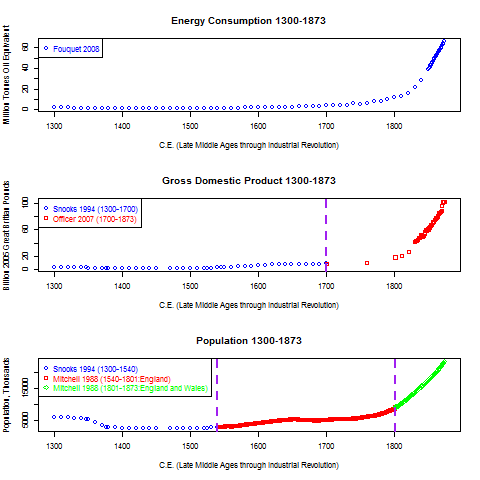
\includegraphics[width=0.9\textwidth]{overallLevels}
\end{figure}

		\begin{figure}[p!]
		\caption{English real gross domestic product, \\
		levels and per--capita }
		\label{fig:ggdp}		
		\centerline{
		\mbox{\includegraphics[width=0.55\textwidth]{ggdp}}
		\mbox{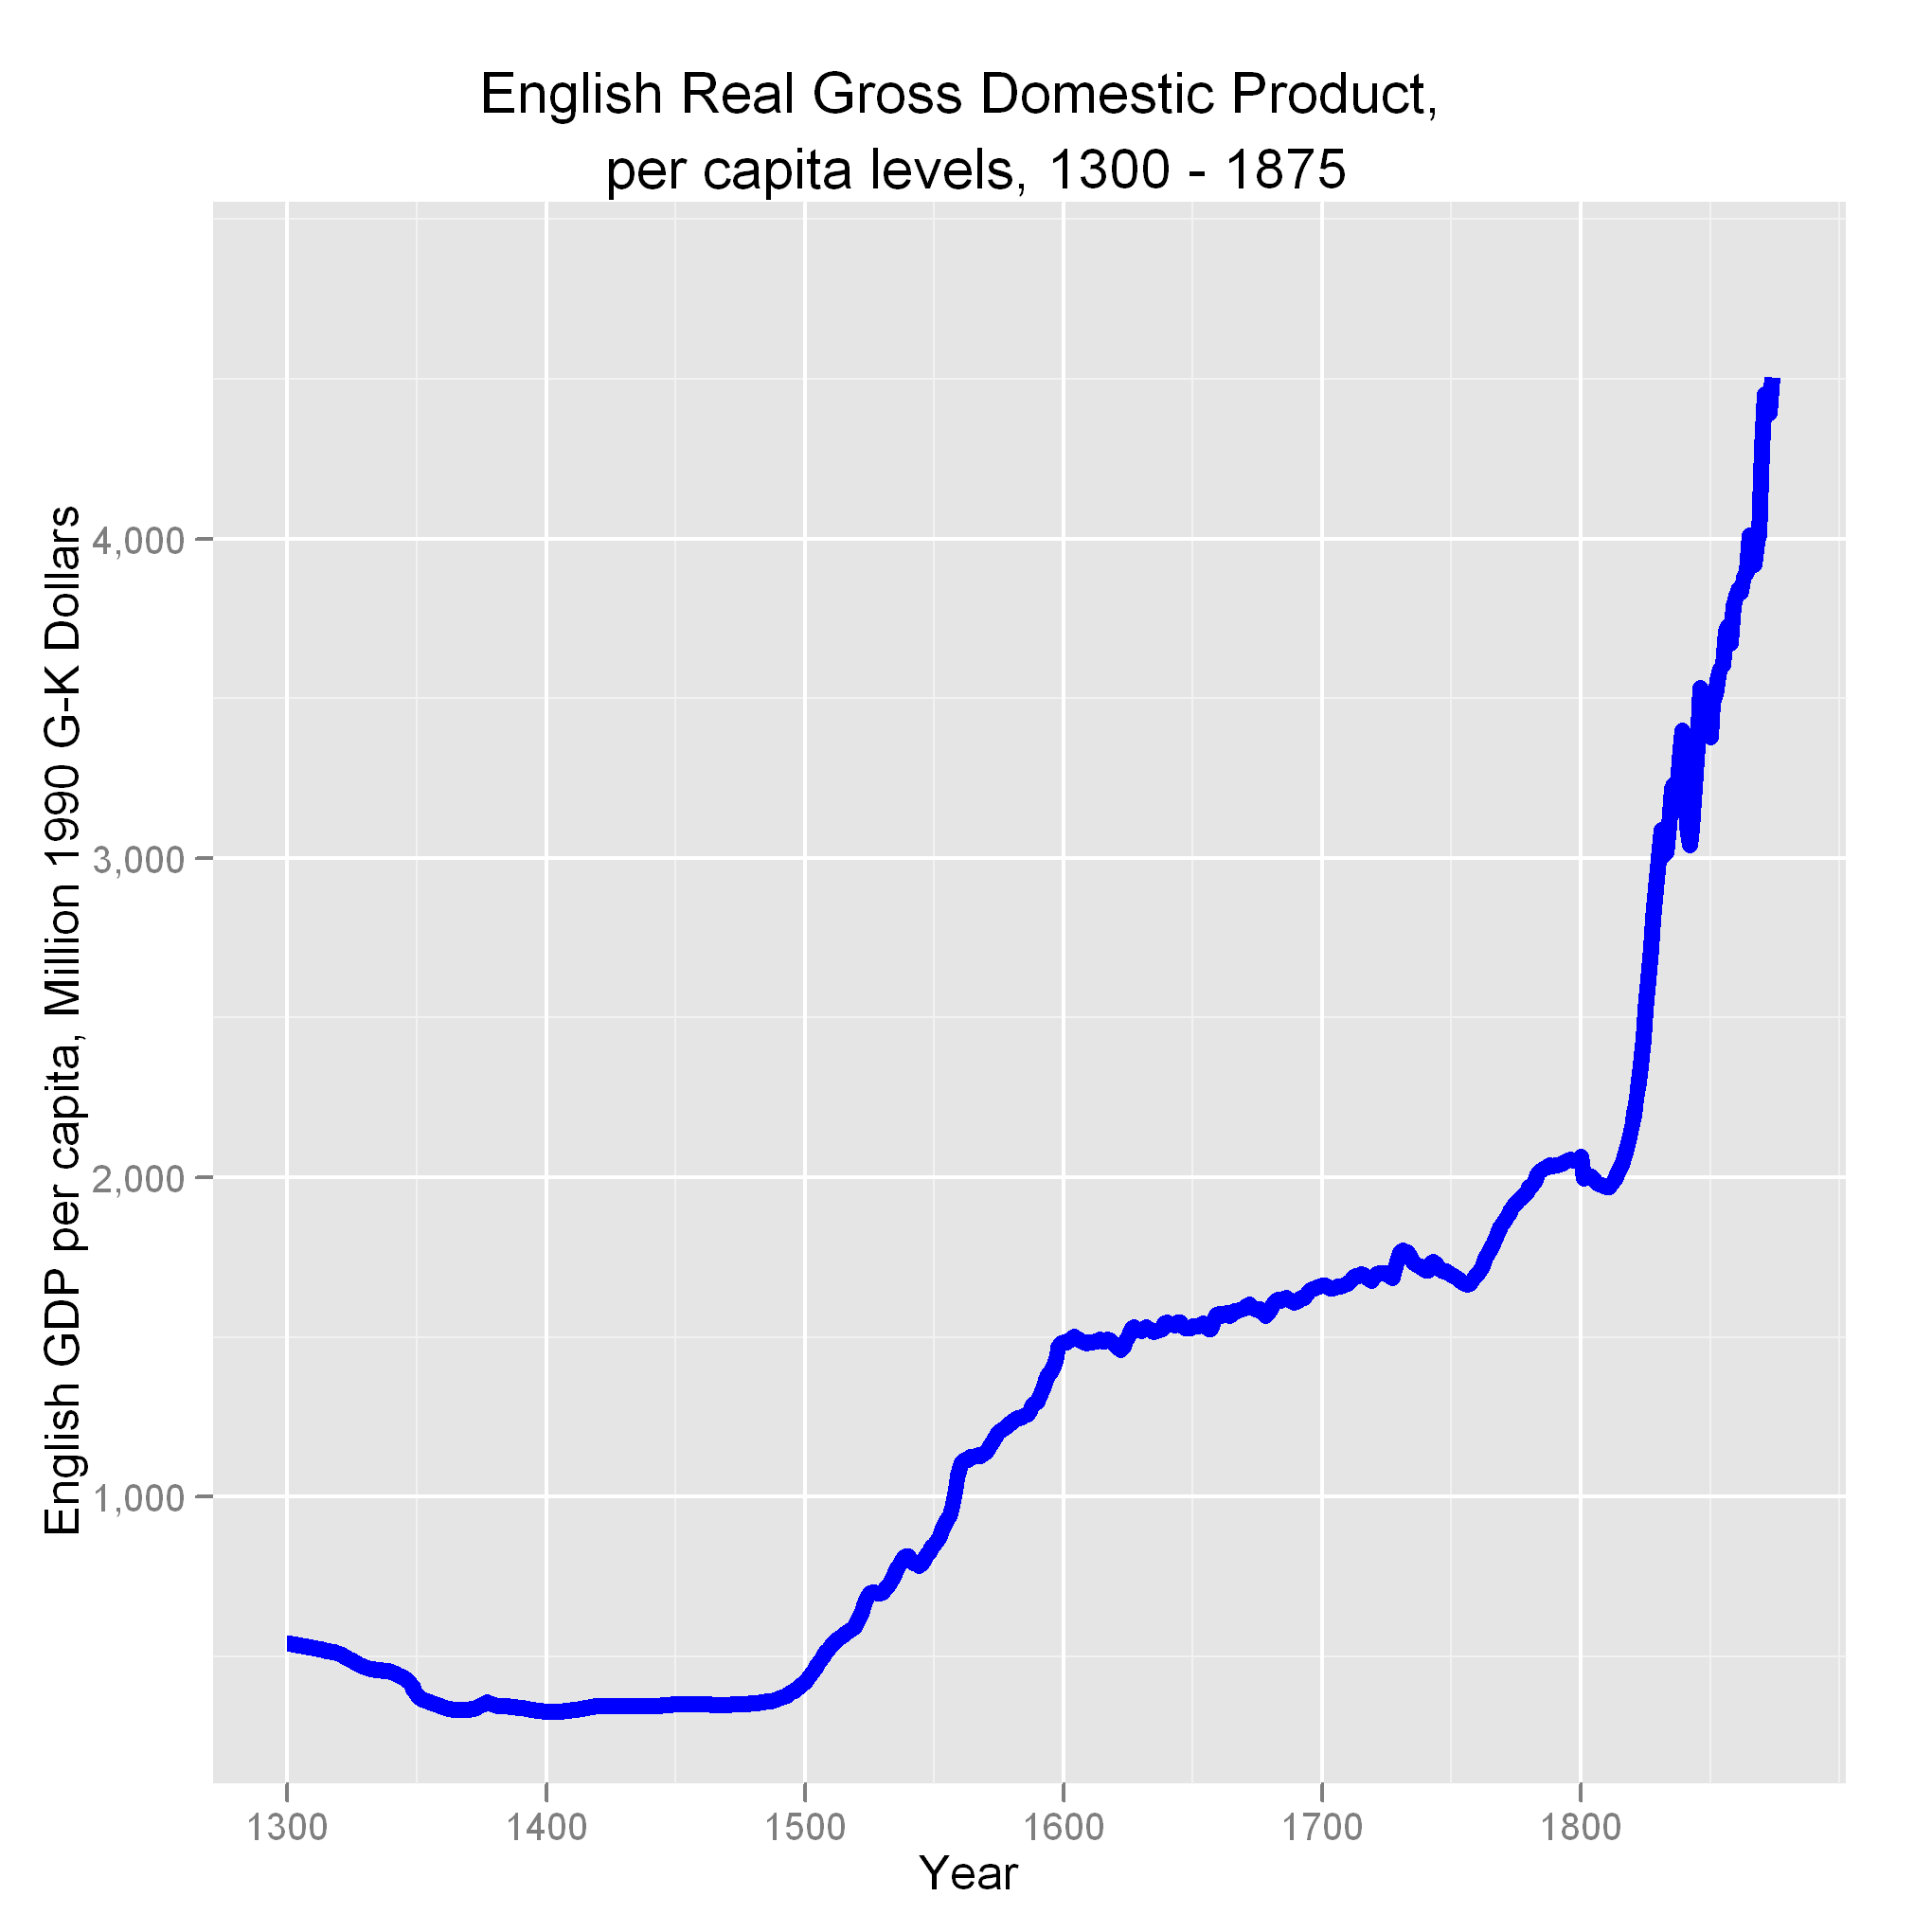
\includegraphics[width=0.55\textwidth]{ggdppop}}
		}
		\end{figure}

		\begin{figure}[p!]
		\caption{English real gross domestic product, \\
		log levels and log per--capita}
		\label{fig:gdpLog}		
		\centerline{
		\mbox{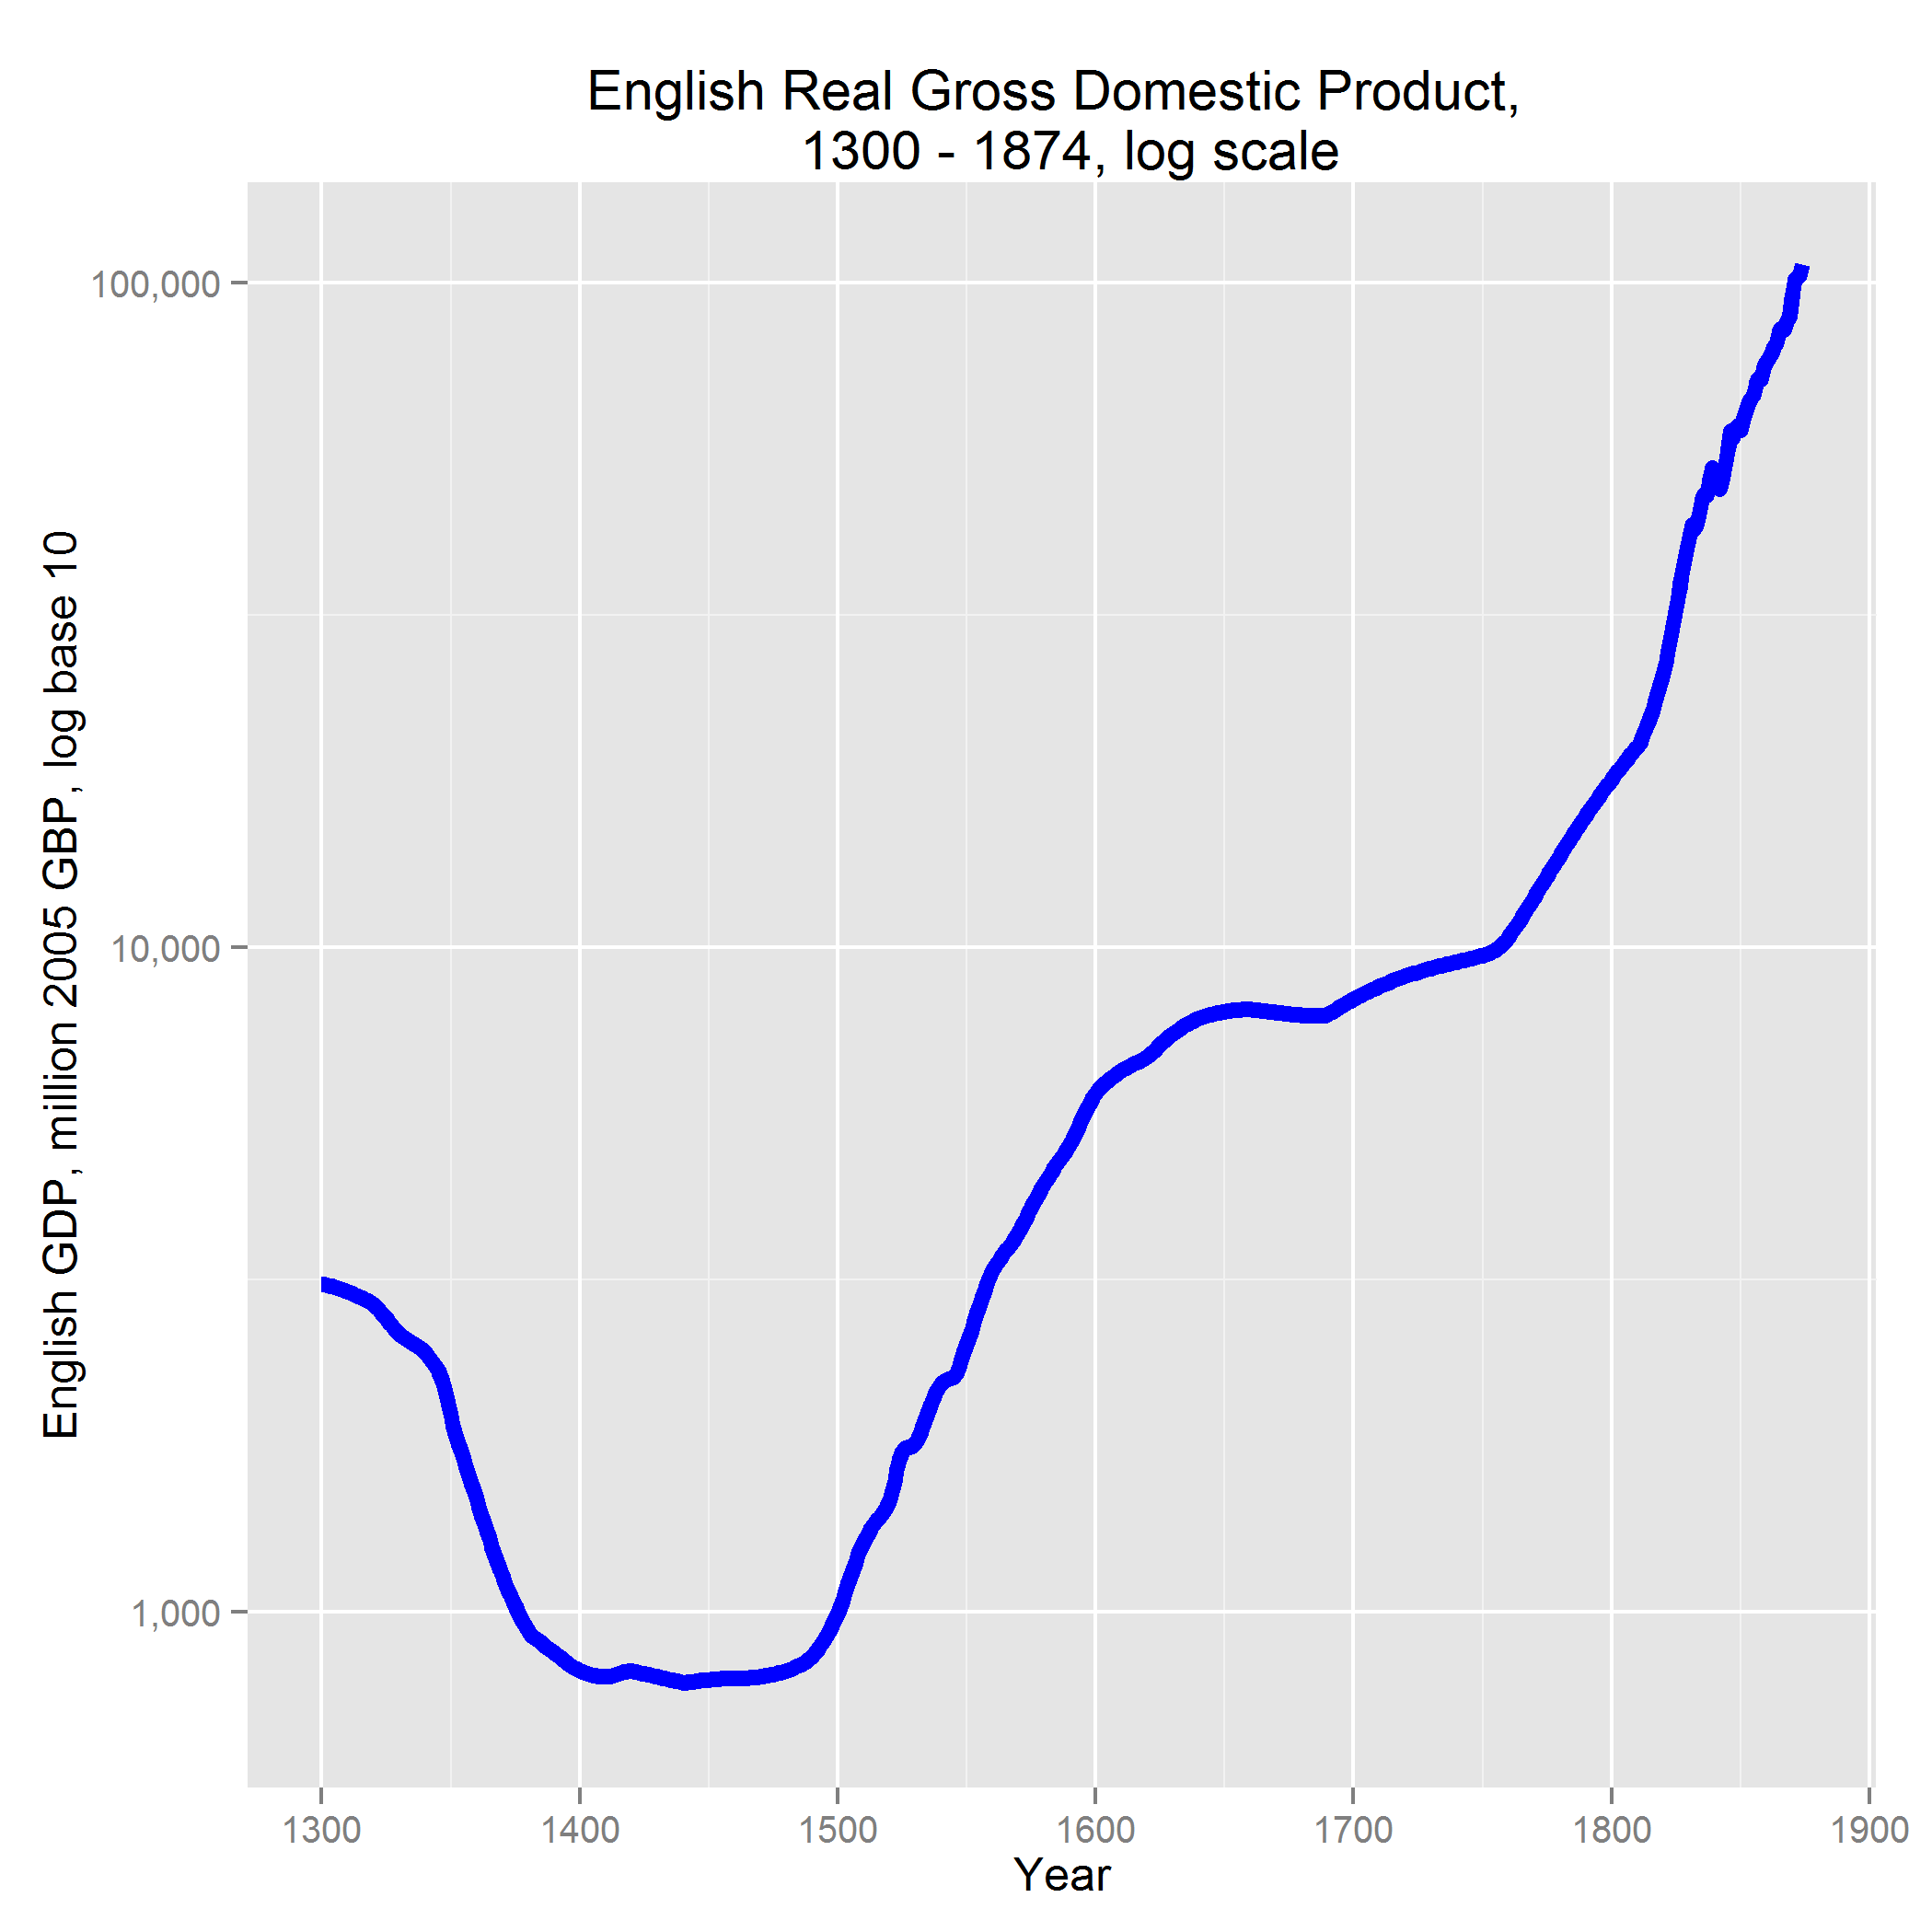
\includegraphics[width=0.55\textwidth]{gdpLog}}
		\mbox{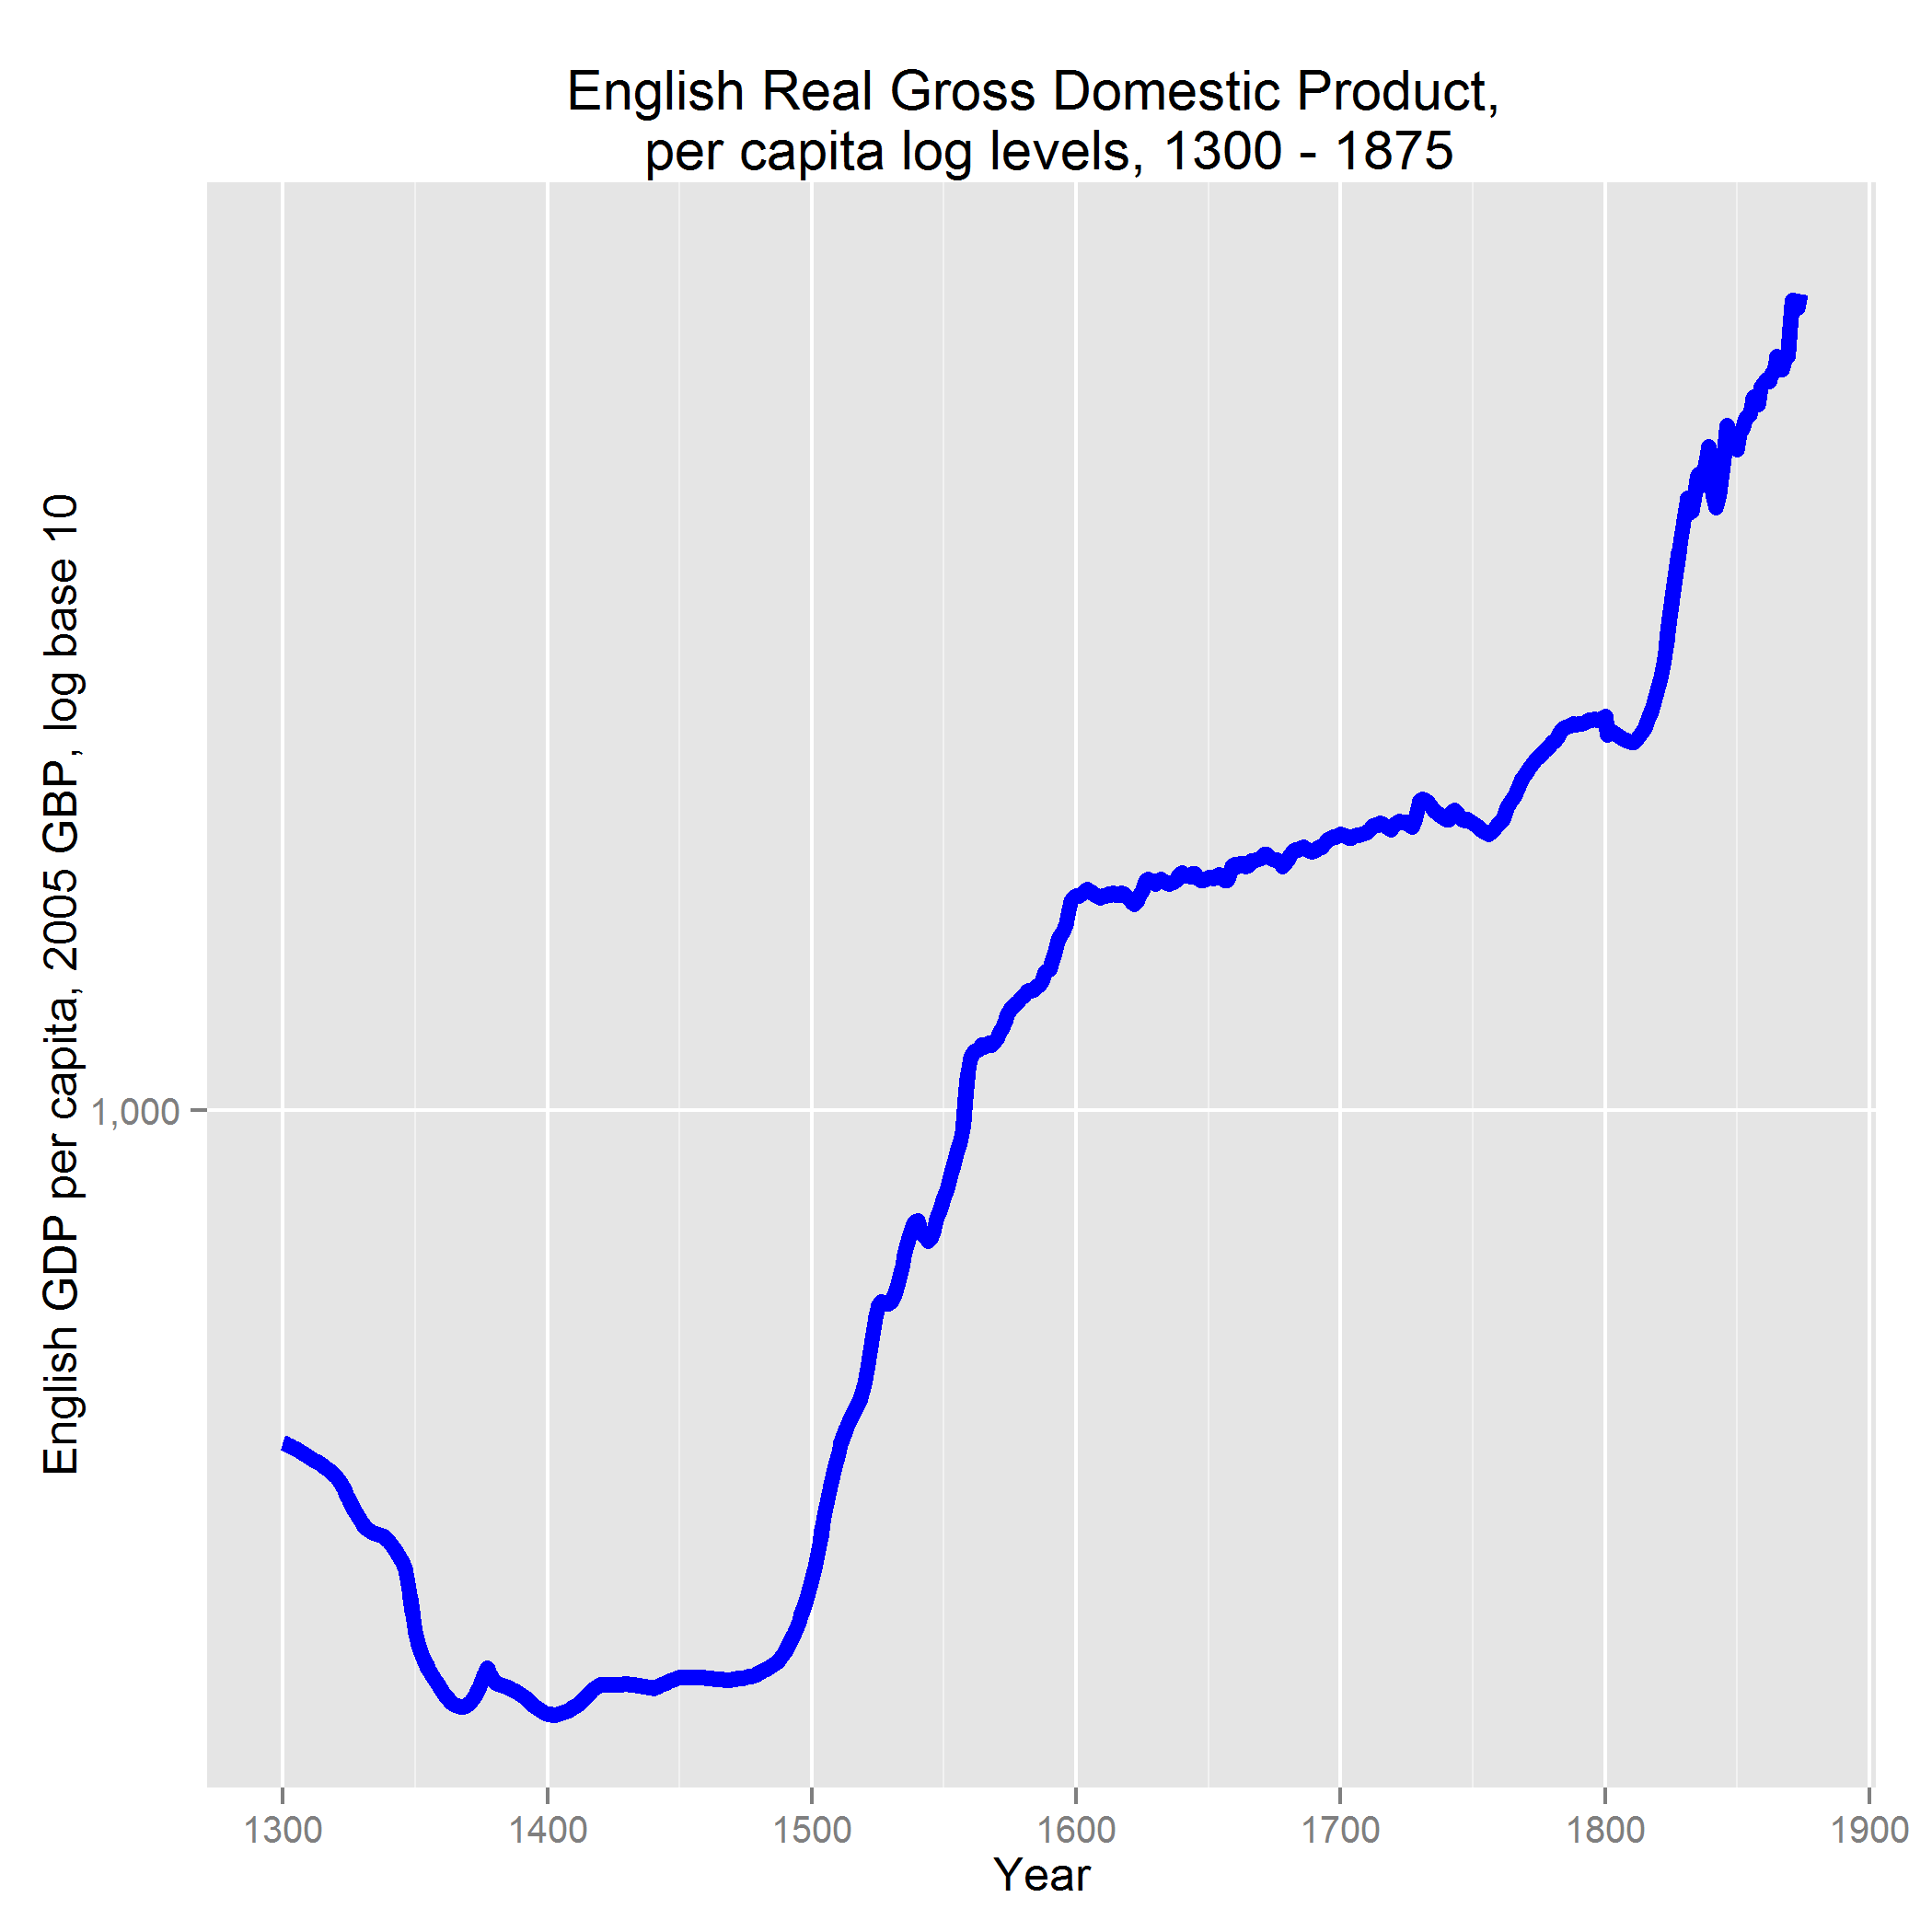
\includegraphics[width=0.55\textwidth]{gdpPopLog}}
		}
		\end{figure}

\begin{figure}[p!]
\center
\caption{Log of population, with structural breaks}
\label{fig:popLog}
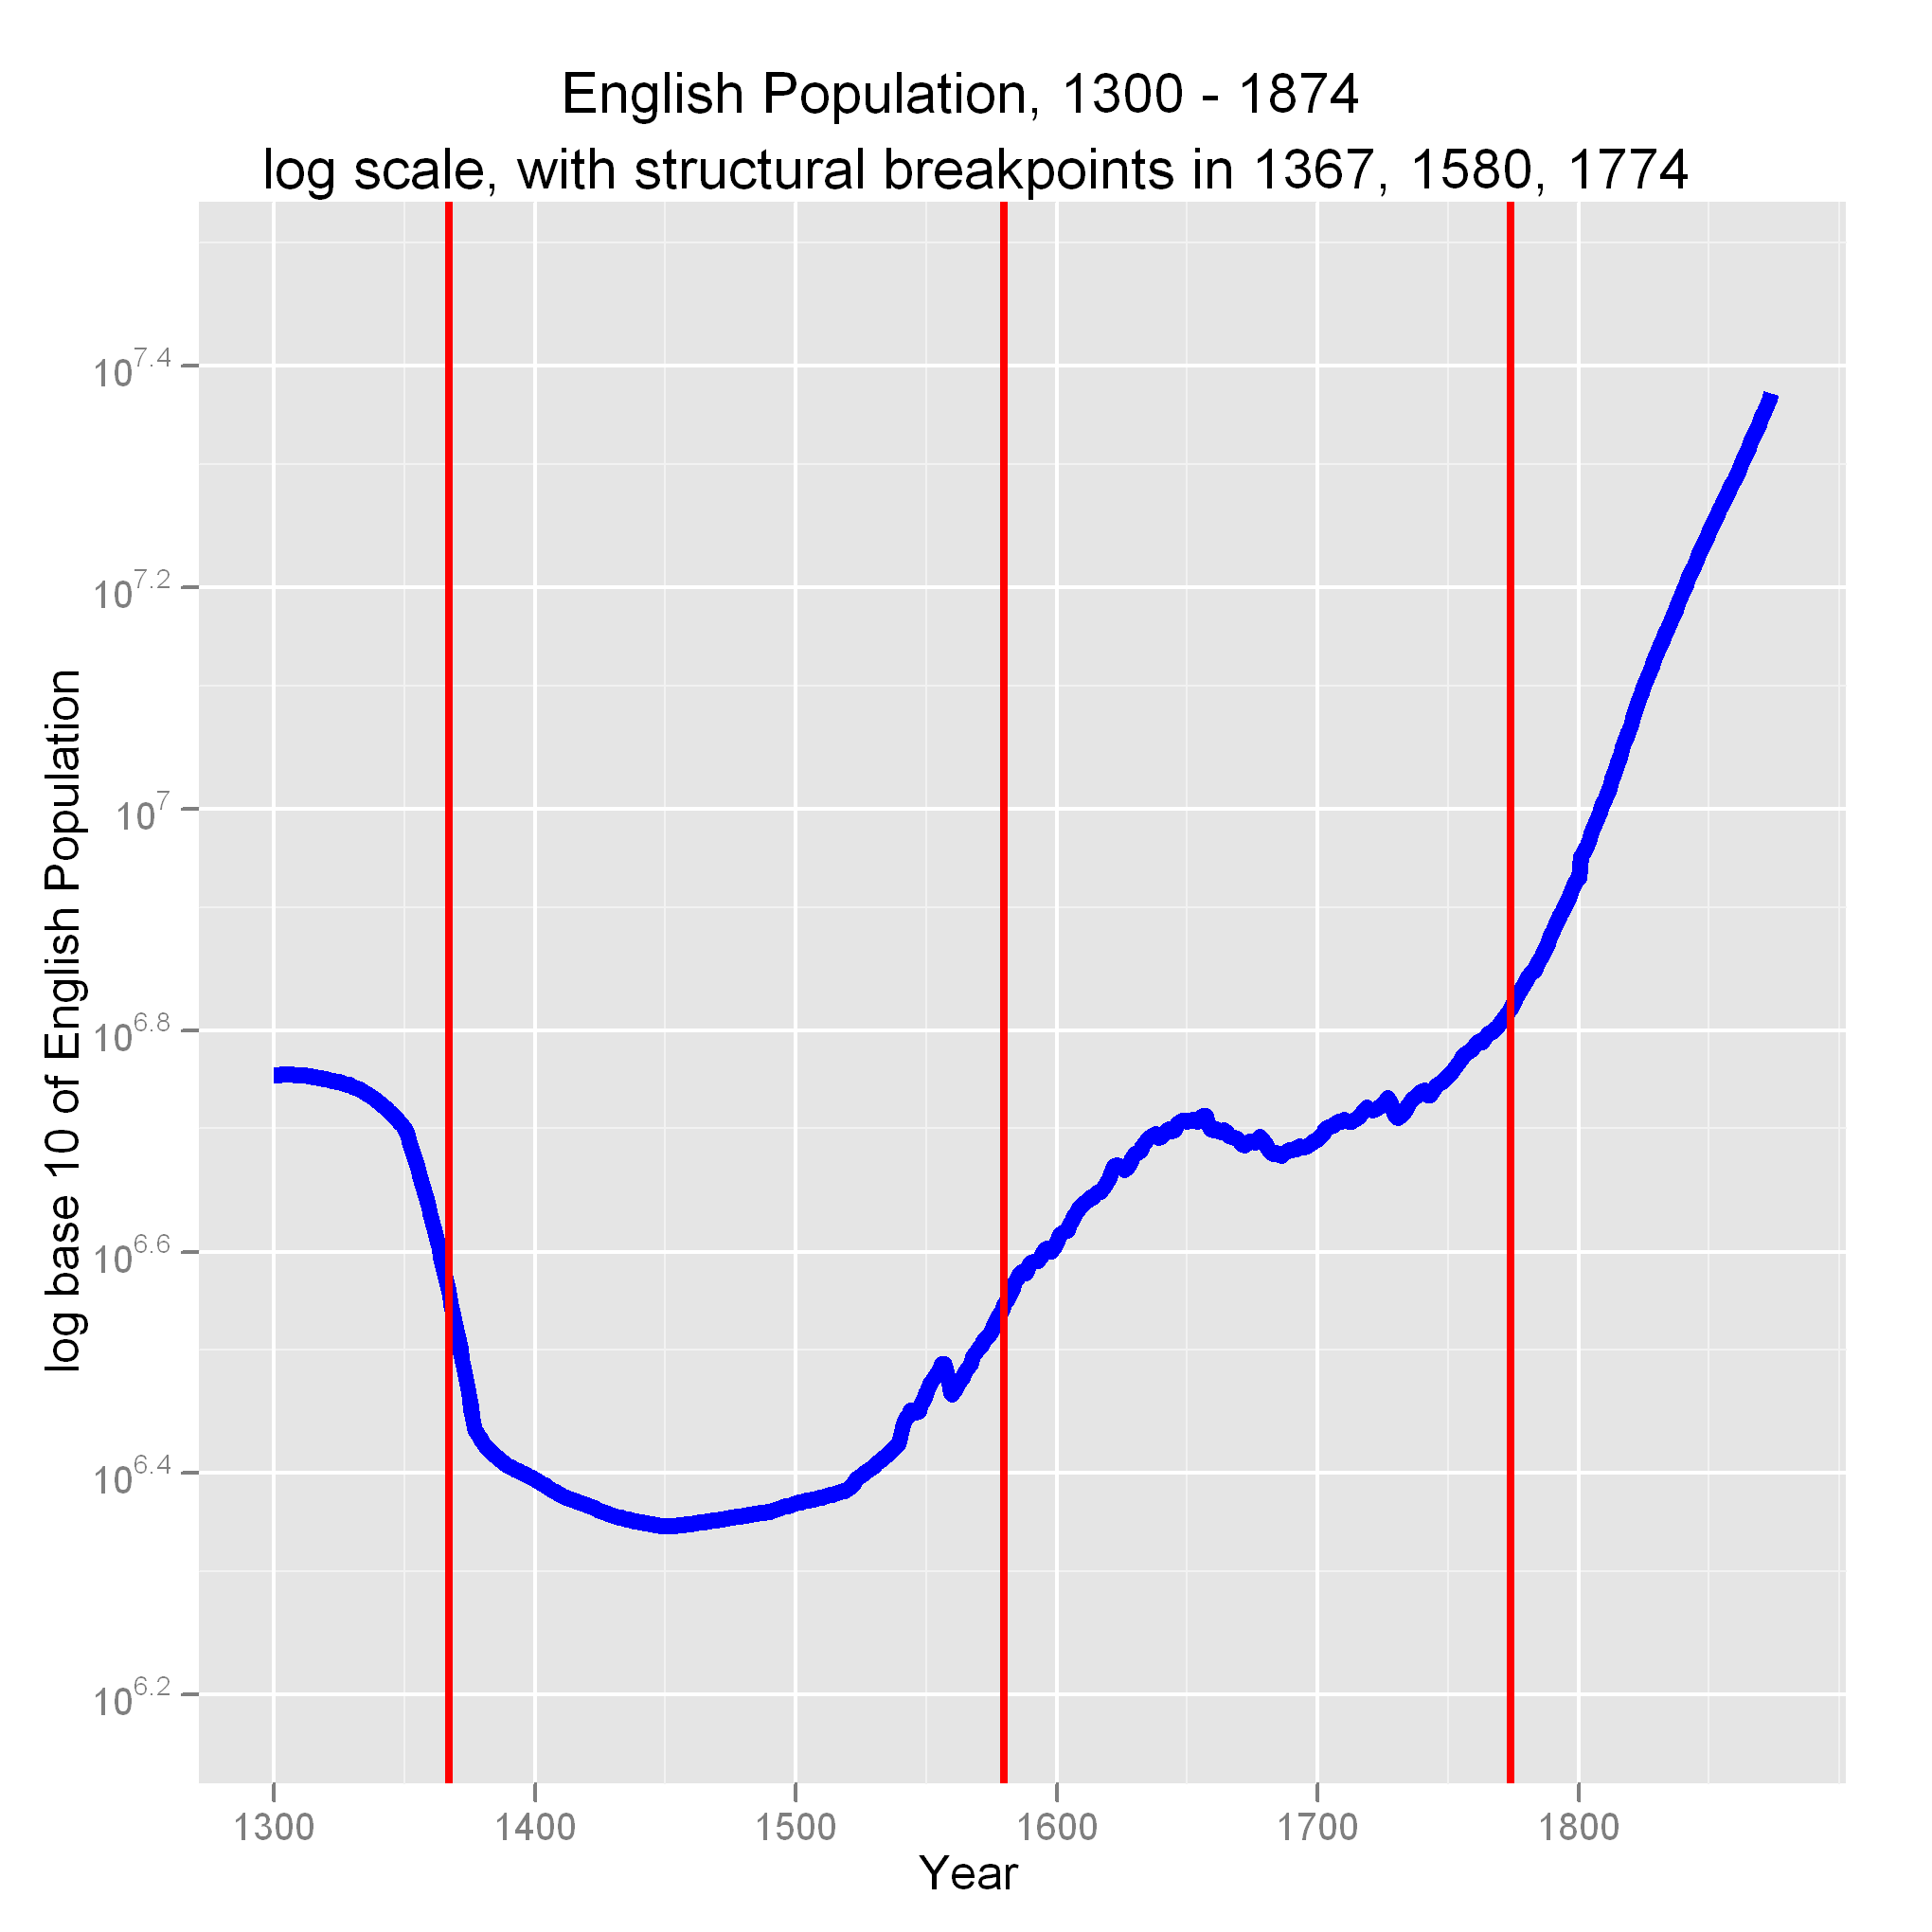
\includegraphics[width=0.9\textwidth]{popLog}
\end{figure}

\begin{figure}[p!]
\center
\caption{Log of energy consumption, with structural breaks}
\label{fig:energyLog}
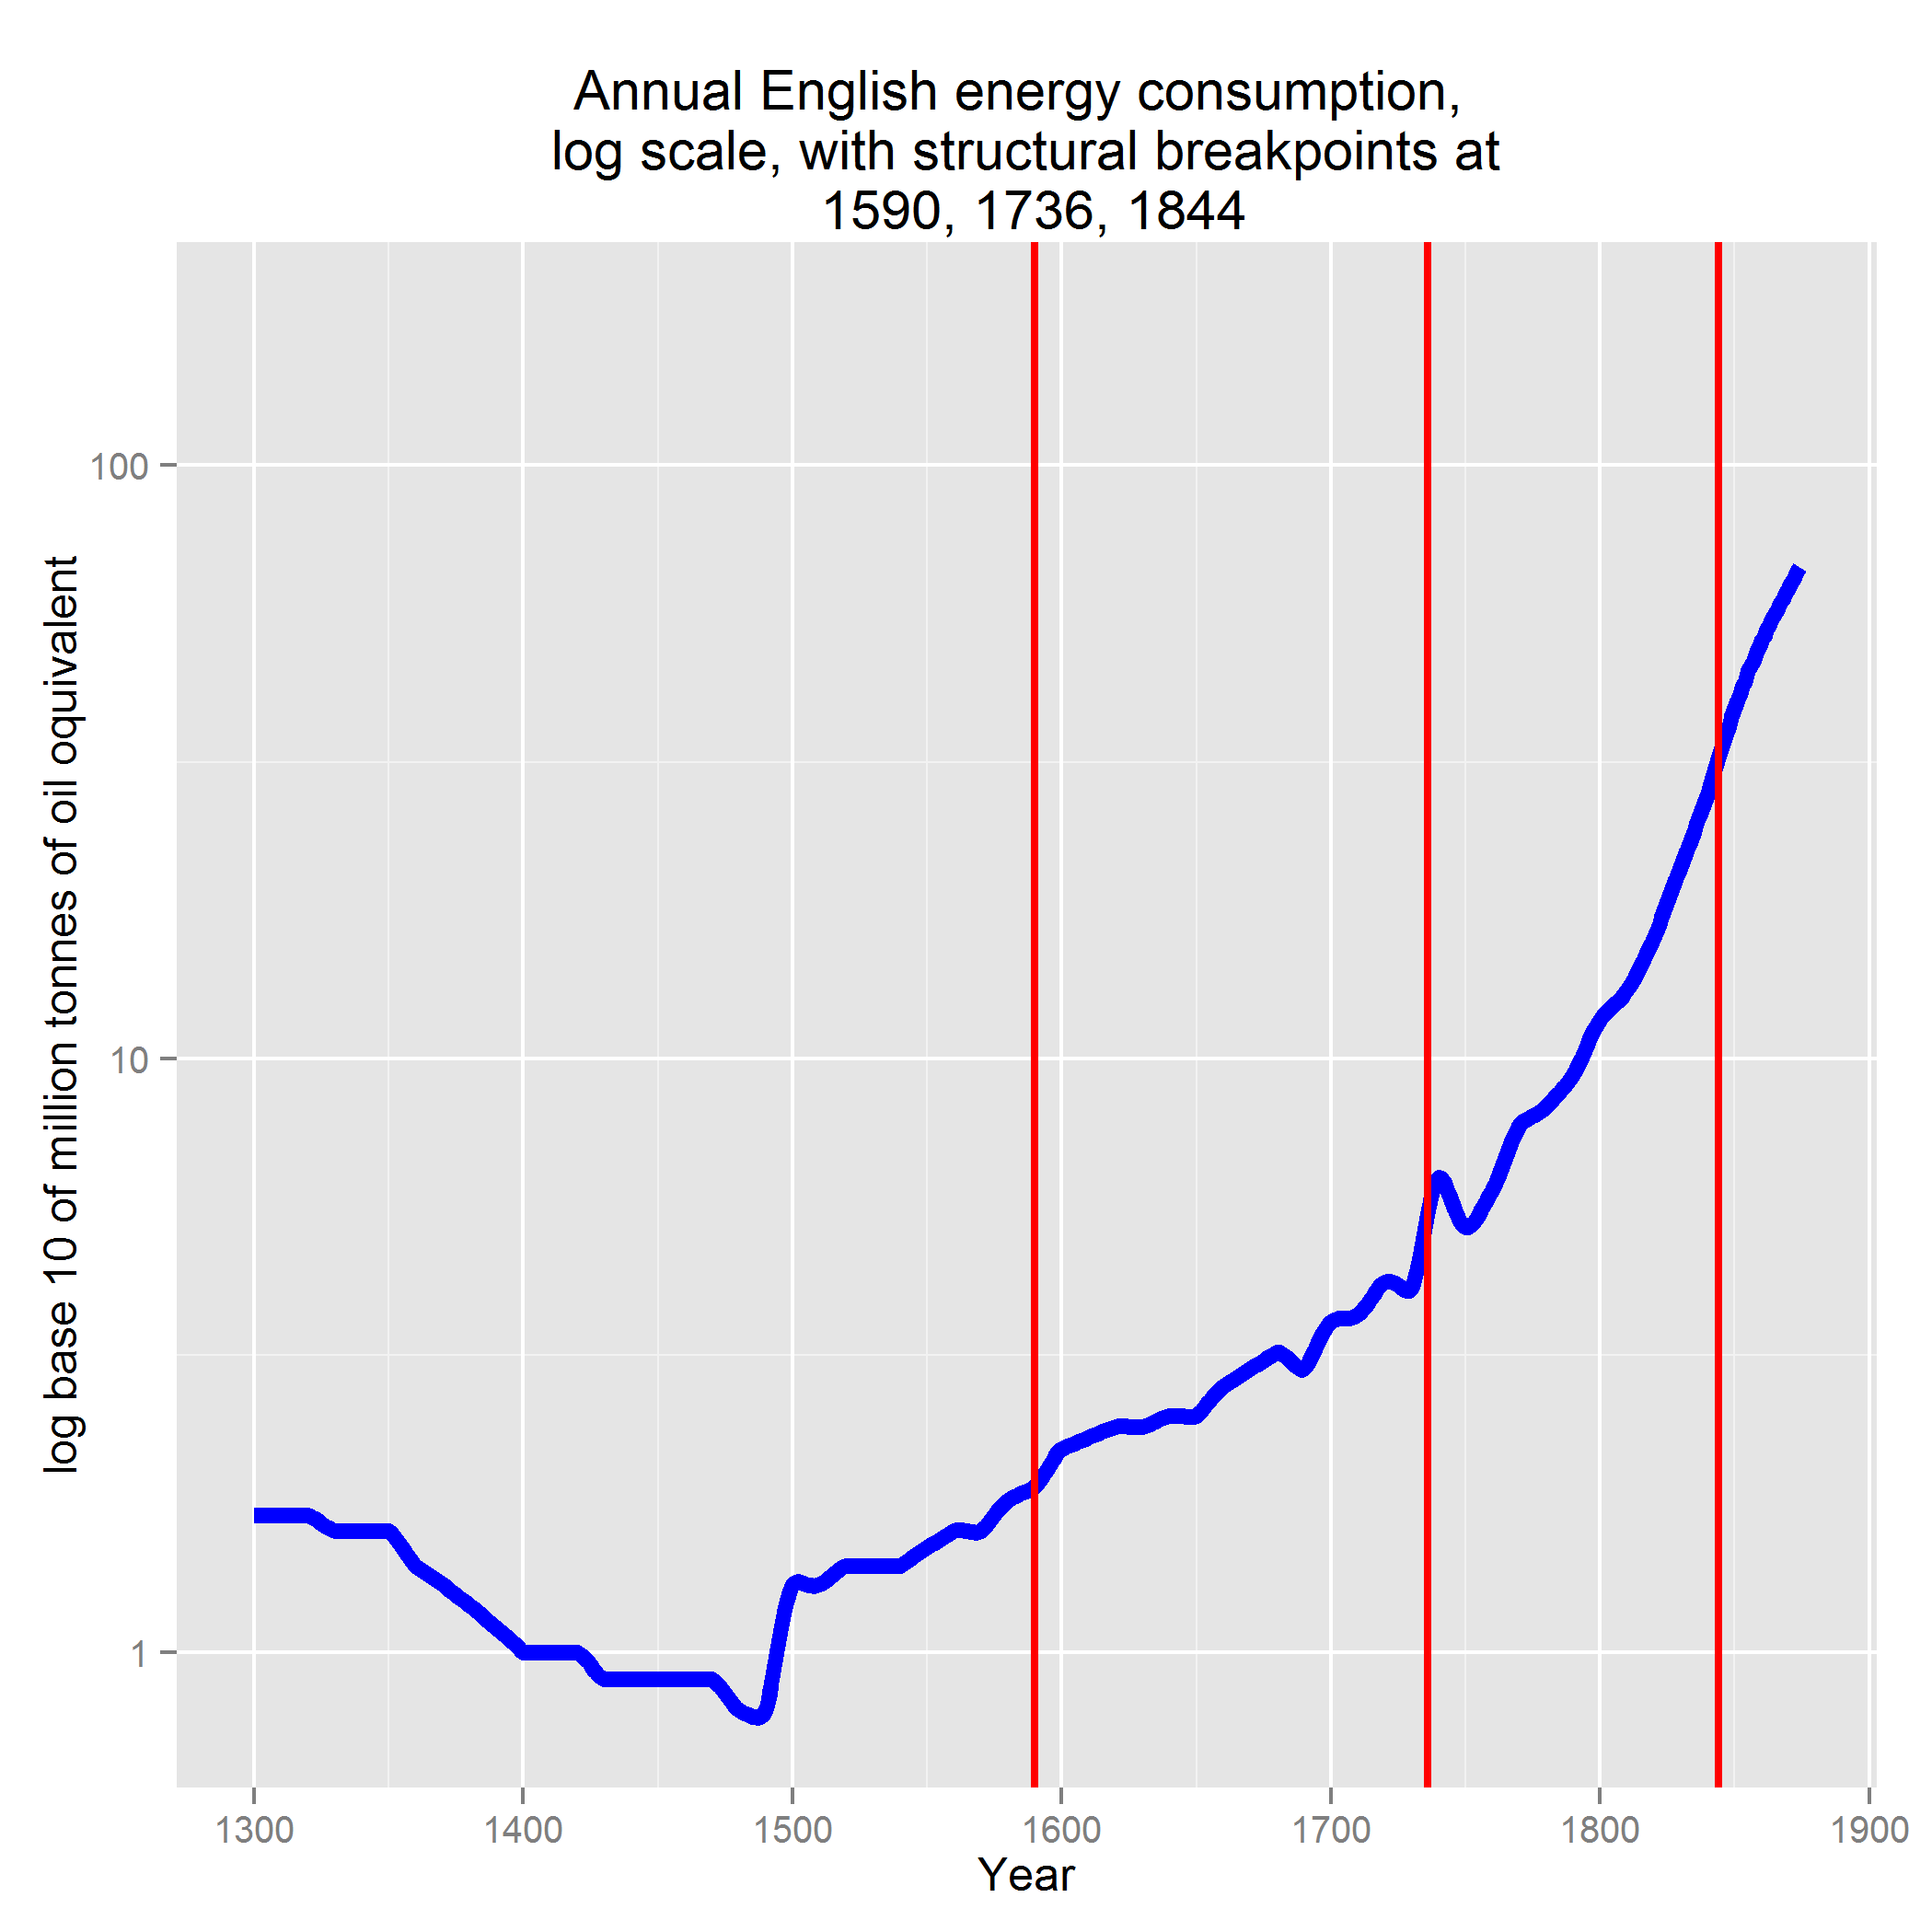
\includegraphics[width=0.9\textwidth]{energyLog1.png}
\end{figure}

\begin{figure}[p!]
\center
\caption{Energy consumption vs. standarized GDP}
\label{fig:energyVsGdp}
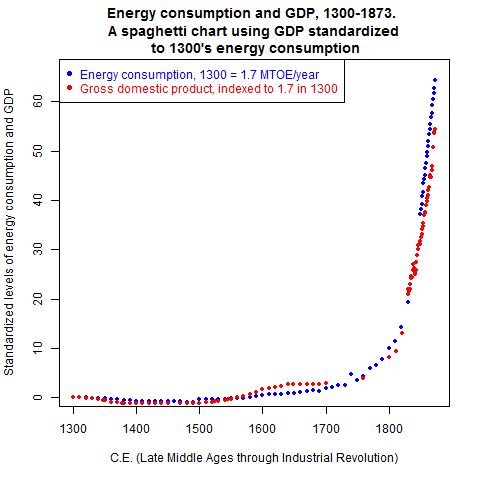
\includegraphics[width=0.9\textwidth]{energyVsGdp}
\end{figure}

\begin{figure}[p!]
\center
\caption{Energy consumption vs. standardized GDP, differences}
\label{fig:energyVsGdpDiff}
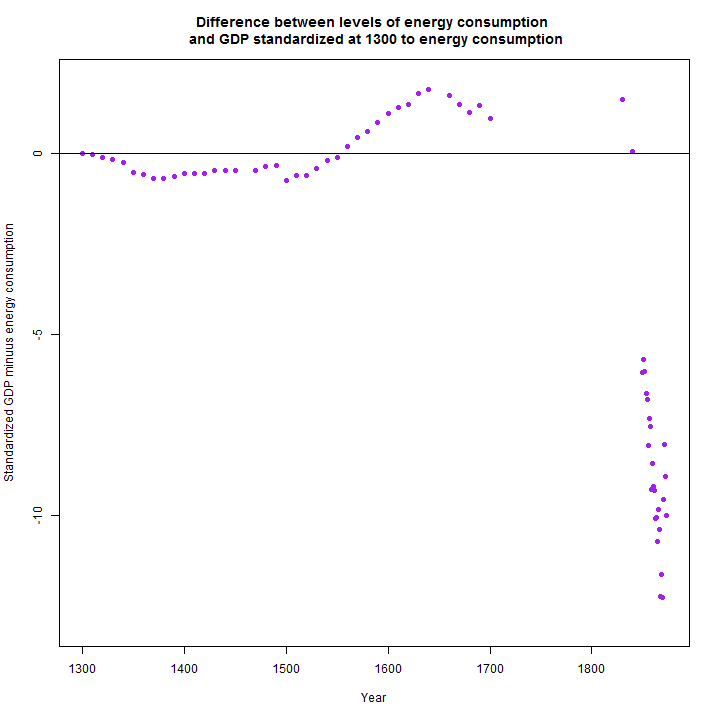
\includegraphics[width=0.9\textwidth]{energyVsGdpDiff}
\end{figure}

\begin{figure}[p!]
\center
\caption{Scatterplot of energy consumption vs. GDP}
\label{fig:scatterplot}
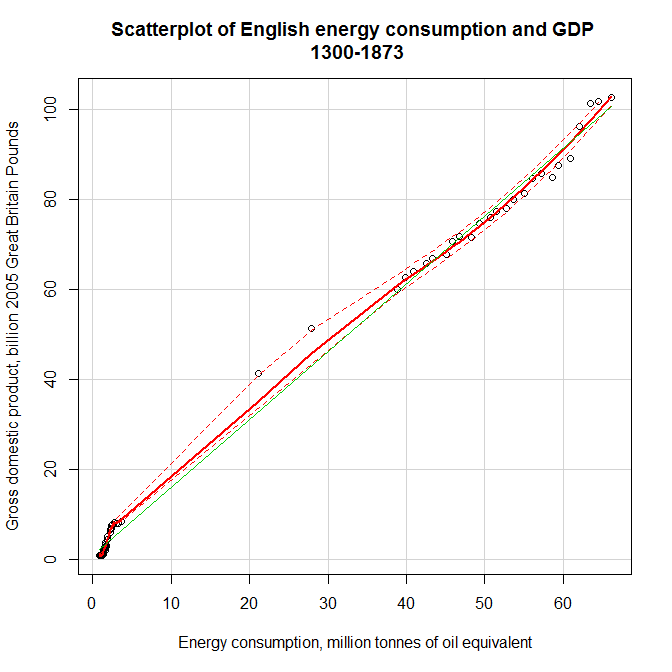
\includegraphics[width=0.9\textwidth]{scatterplot.png}
\end{figure}

\begin{figure}[p!]
		\caption{Structural break comparison}
		\label{fig:structural}		
		\centerline{
		\mbox{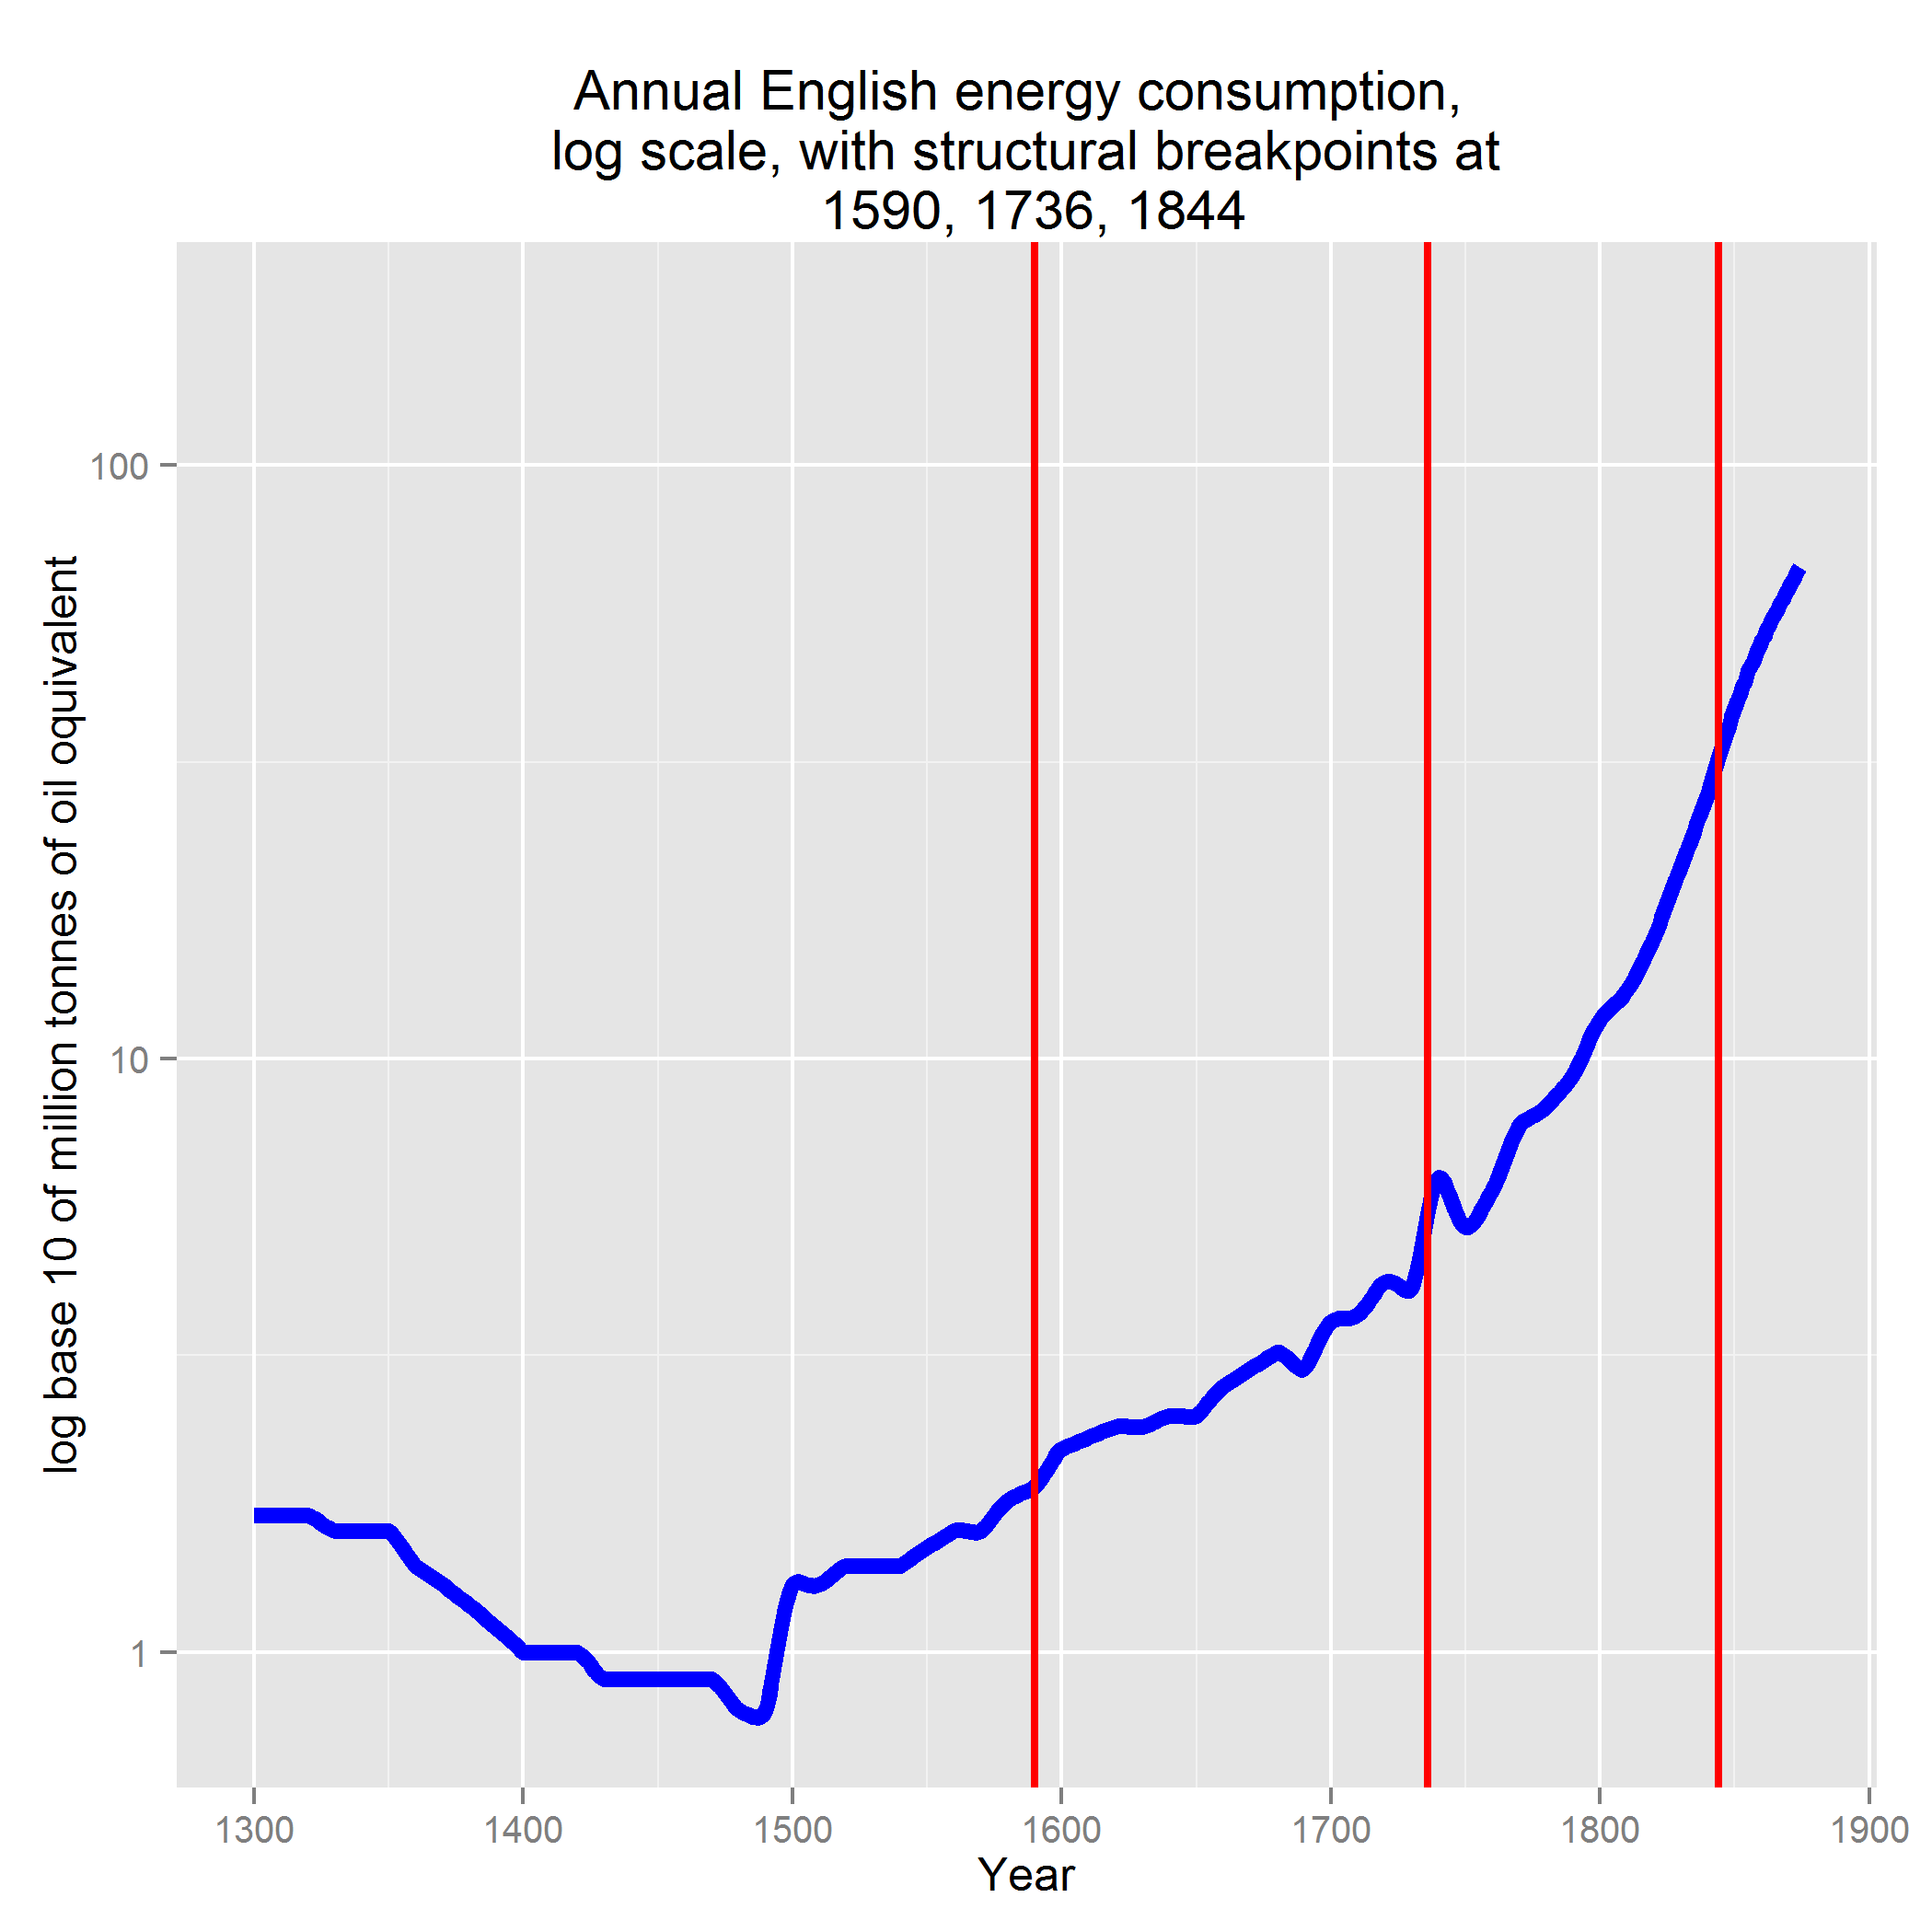
\includegraphics[width=0.33\textwidth]{energyLog1}}
		\mbox{\includegraphics[width=0.33\textwidth]{gbpgdplog}}
		\mbox{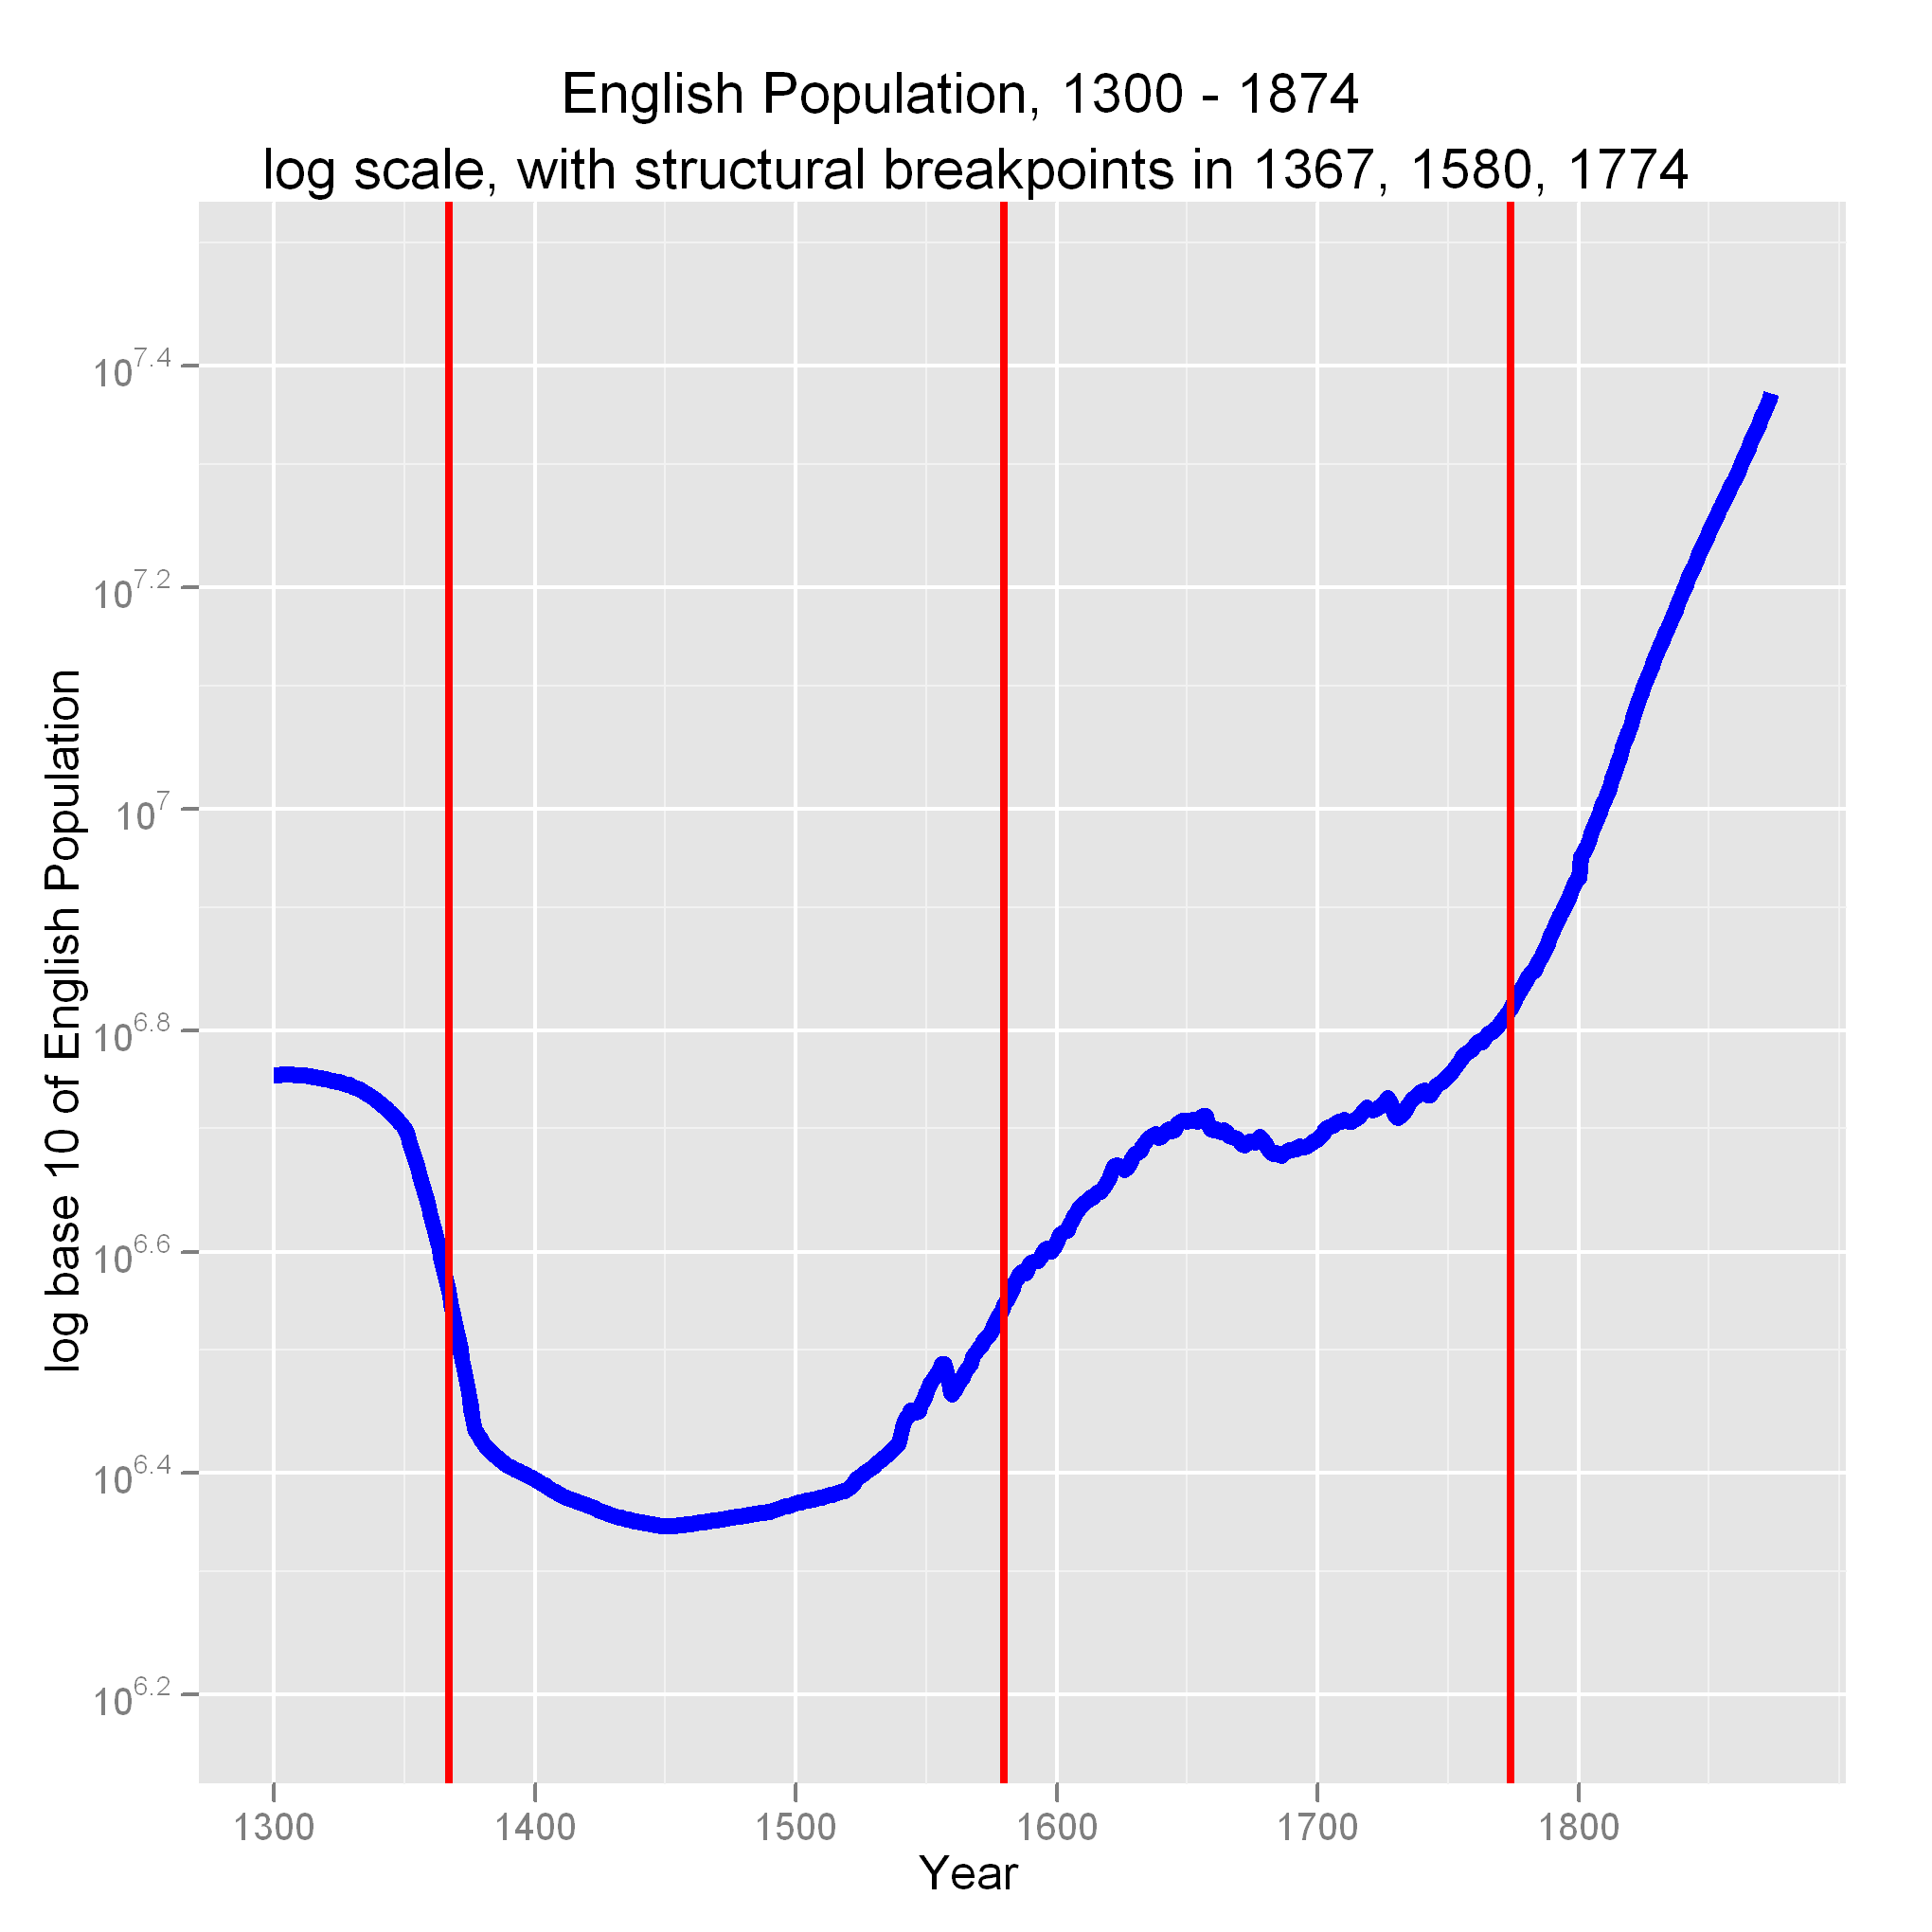
\includegraphics[width=0.33\textwidth]{popLog}}
		}
\end{figure}

\begin{figure}[p!]
\center
\caption{Coal and wood energy sources\\\textit{Source:} Pearson \& Fouquet}
\label{fig:woodCoal}
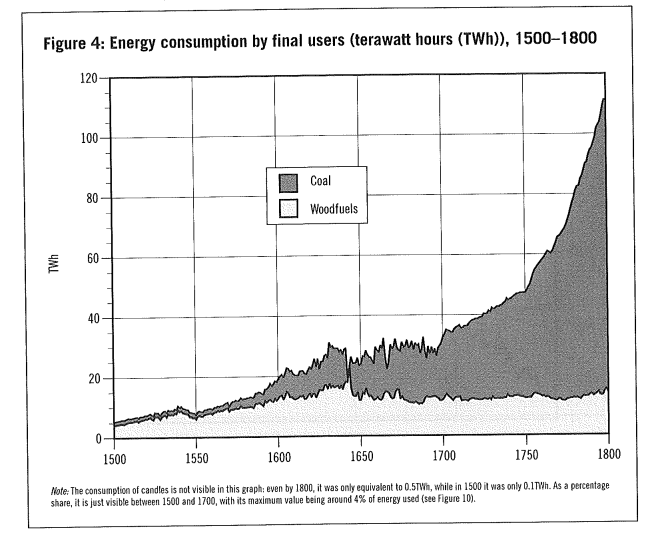
\includegraphics[width=0.9\textwidth]{woodCoal.png}
\end{figure}

\begin{figure}[p!]
		\caption{Aggregate Supply - Aggregate Demand \\ Four energy/GDP regimes}
		\label{fig:asad}		
		\centerline{
		\mbox{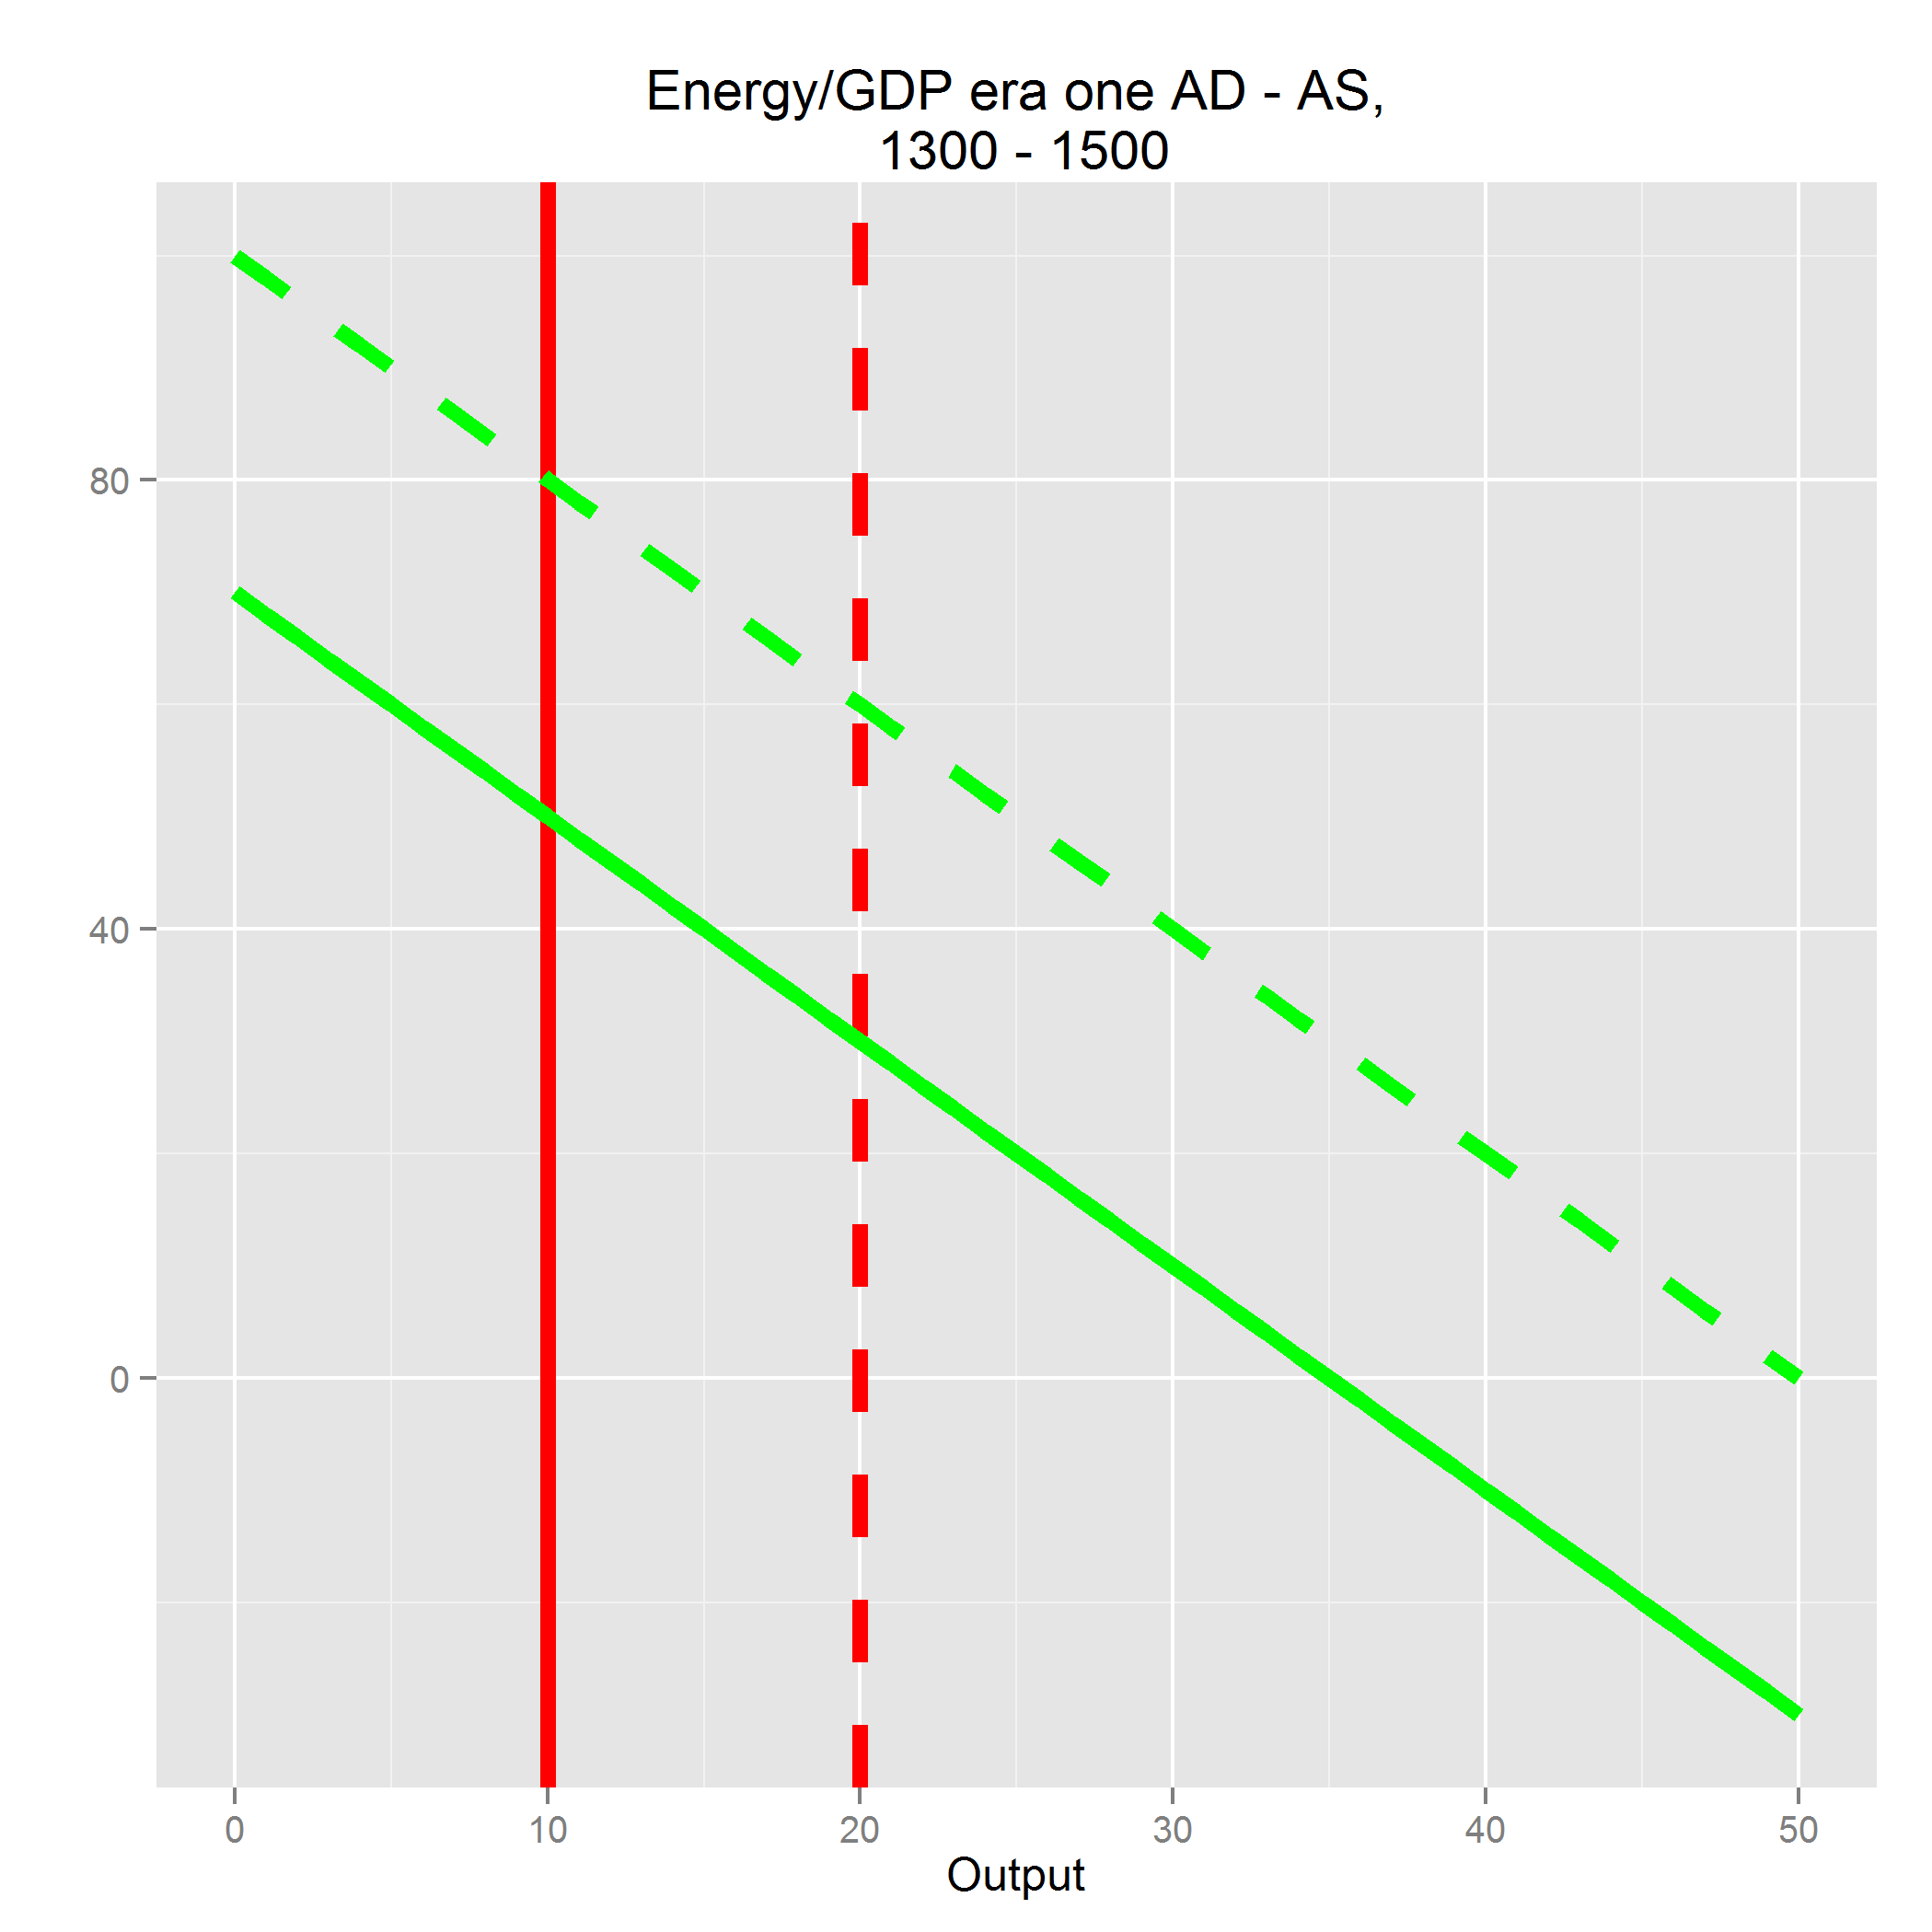
\includegraphics[width=0.25\textwidth]{era1}}
		\mbox{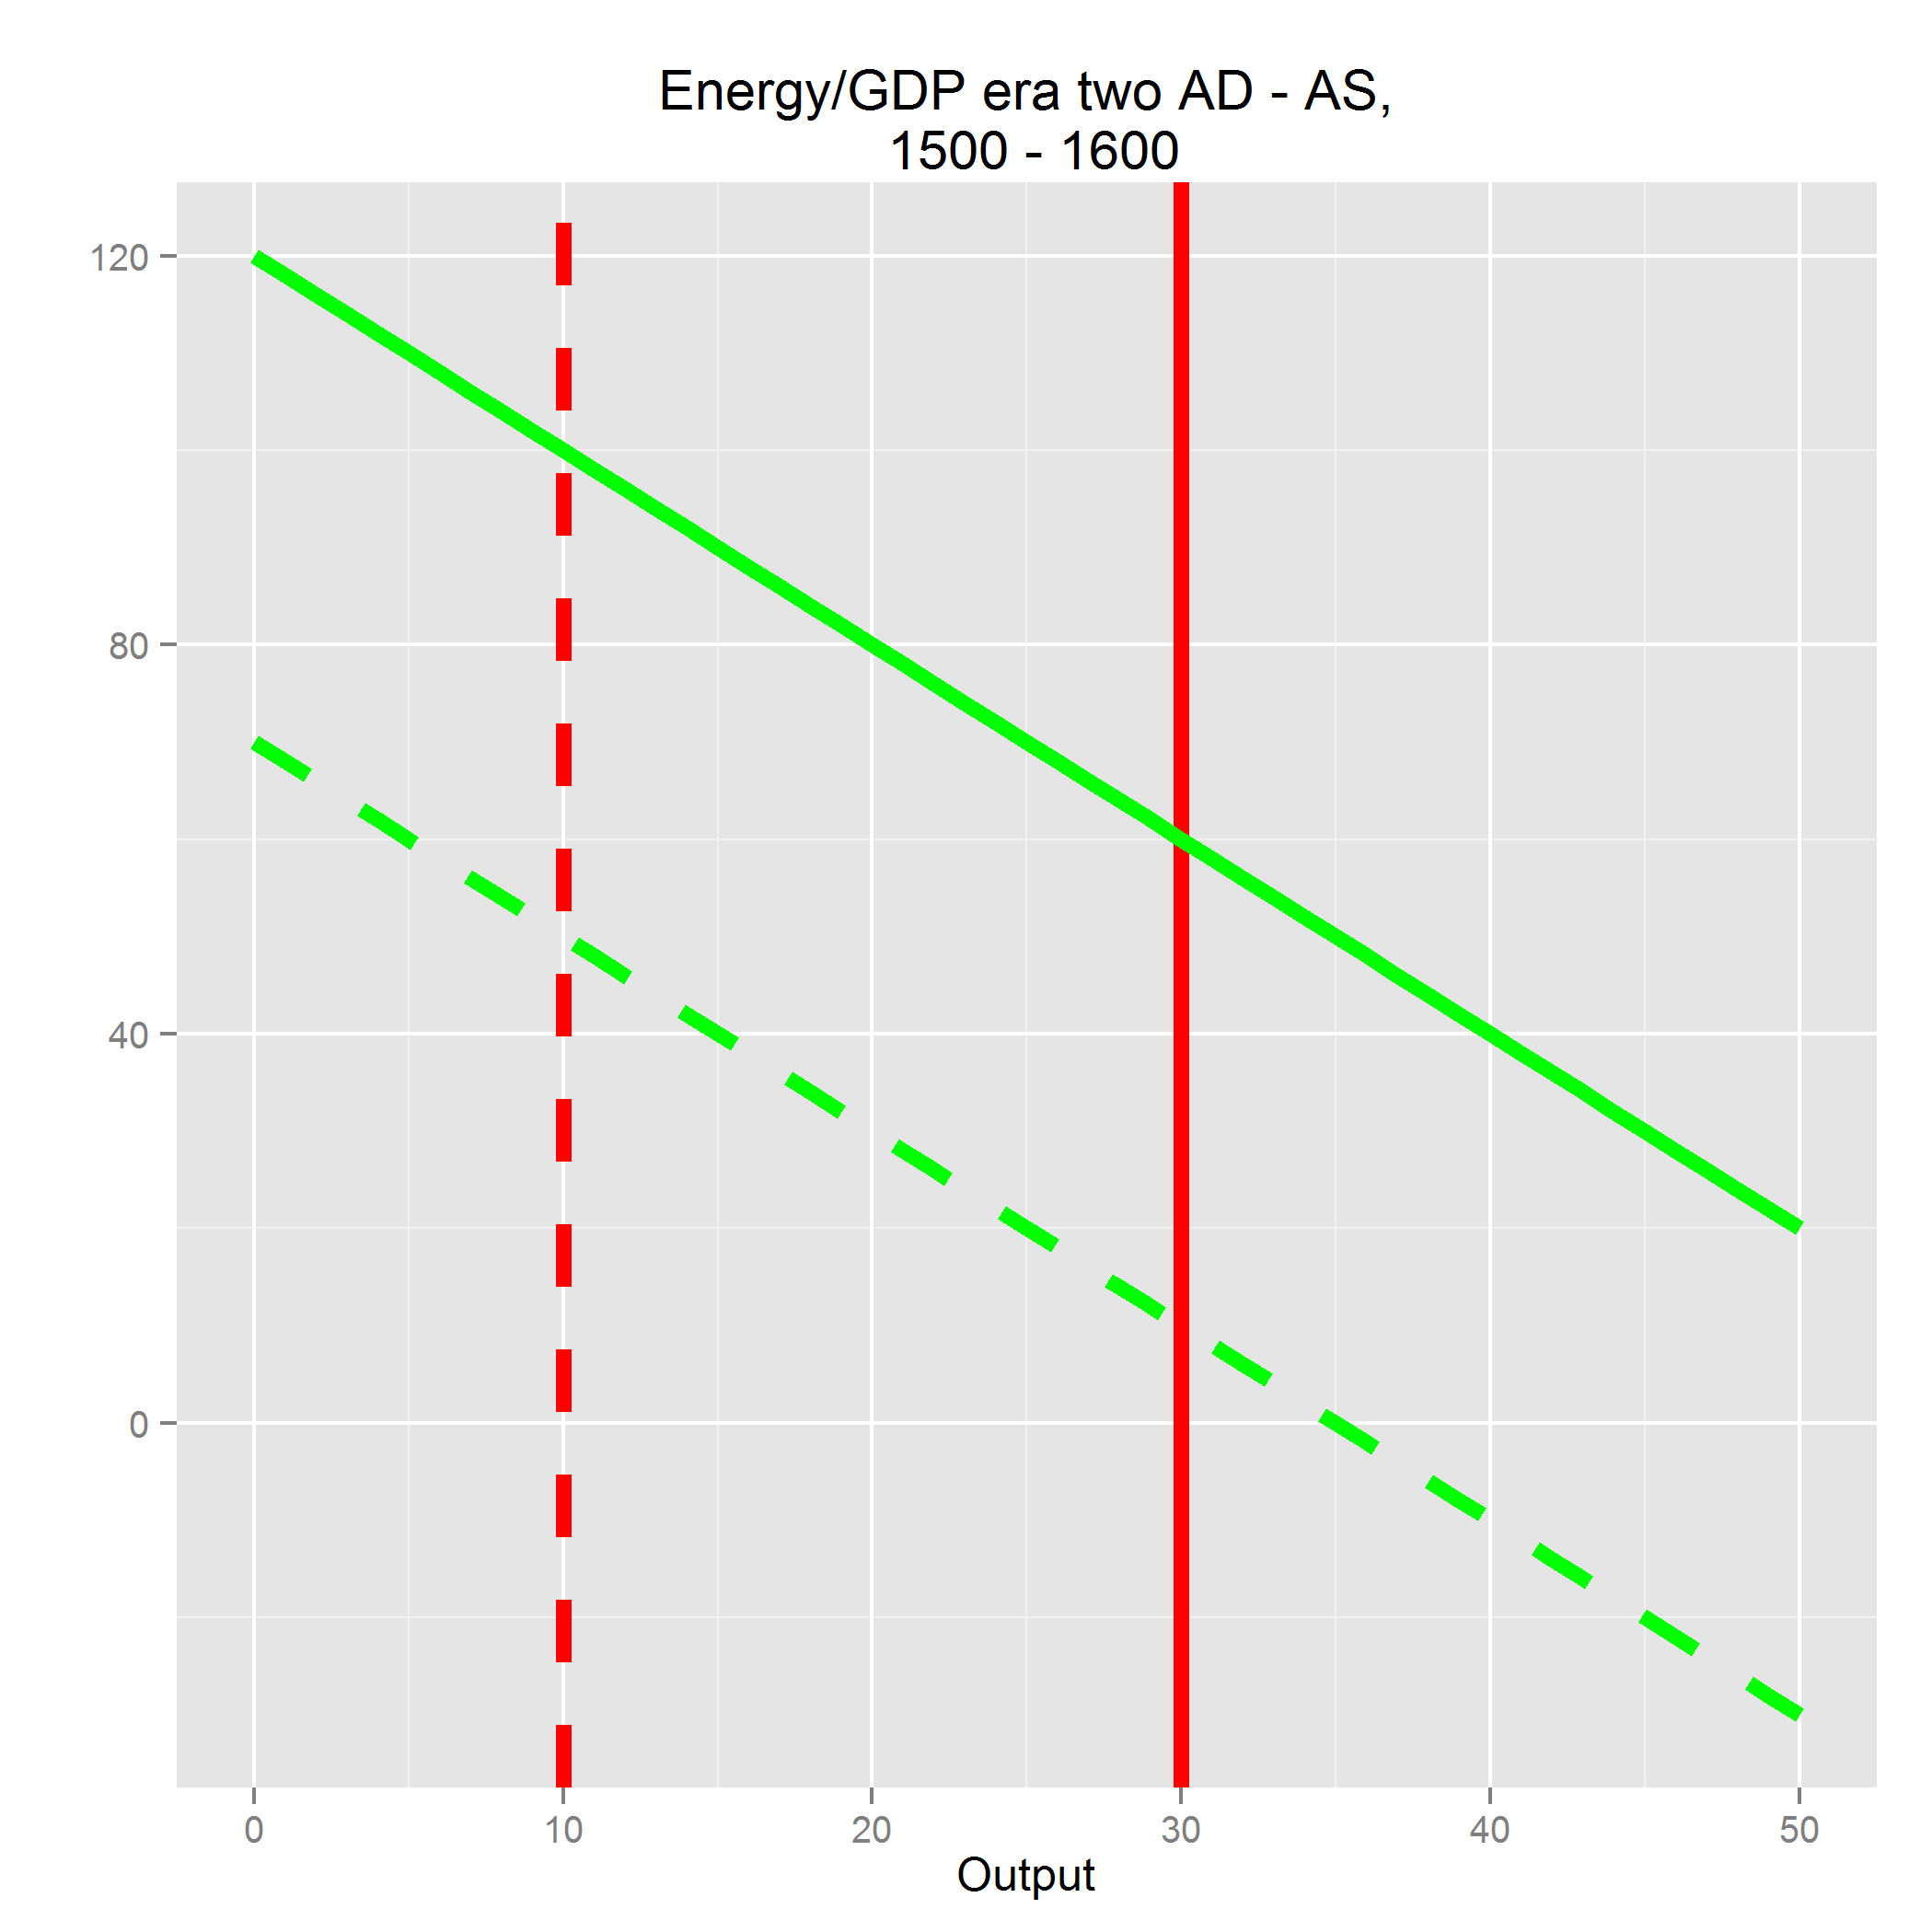
\includegraphics[width=0.25\textwidth]{era2}}
		\mbox{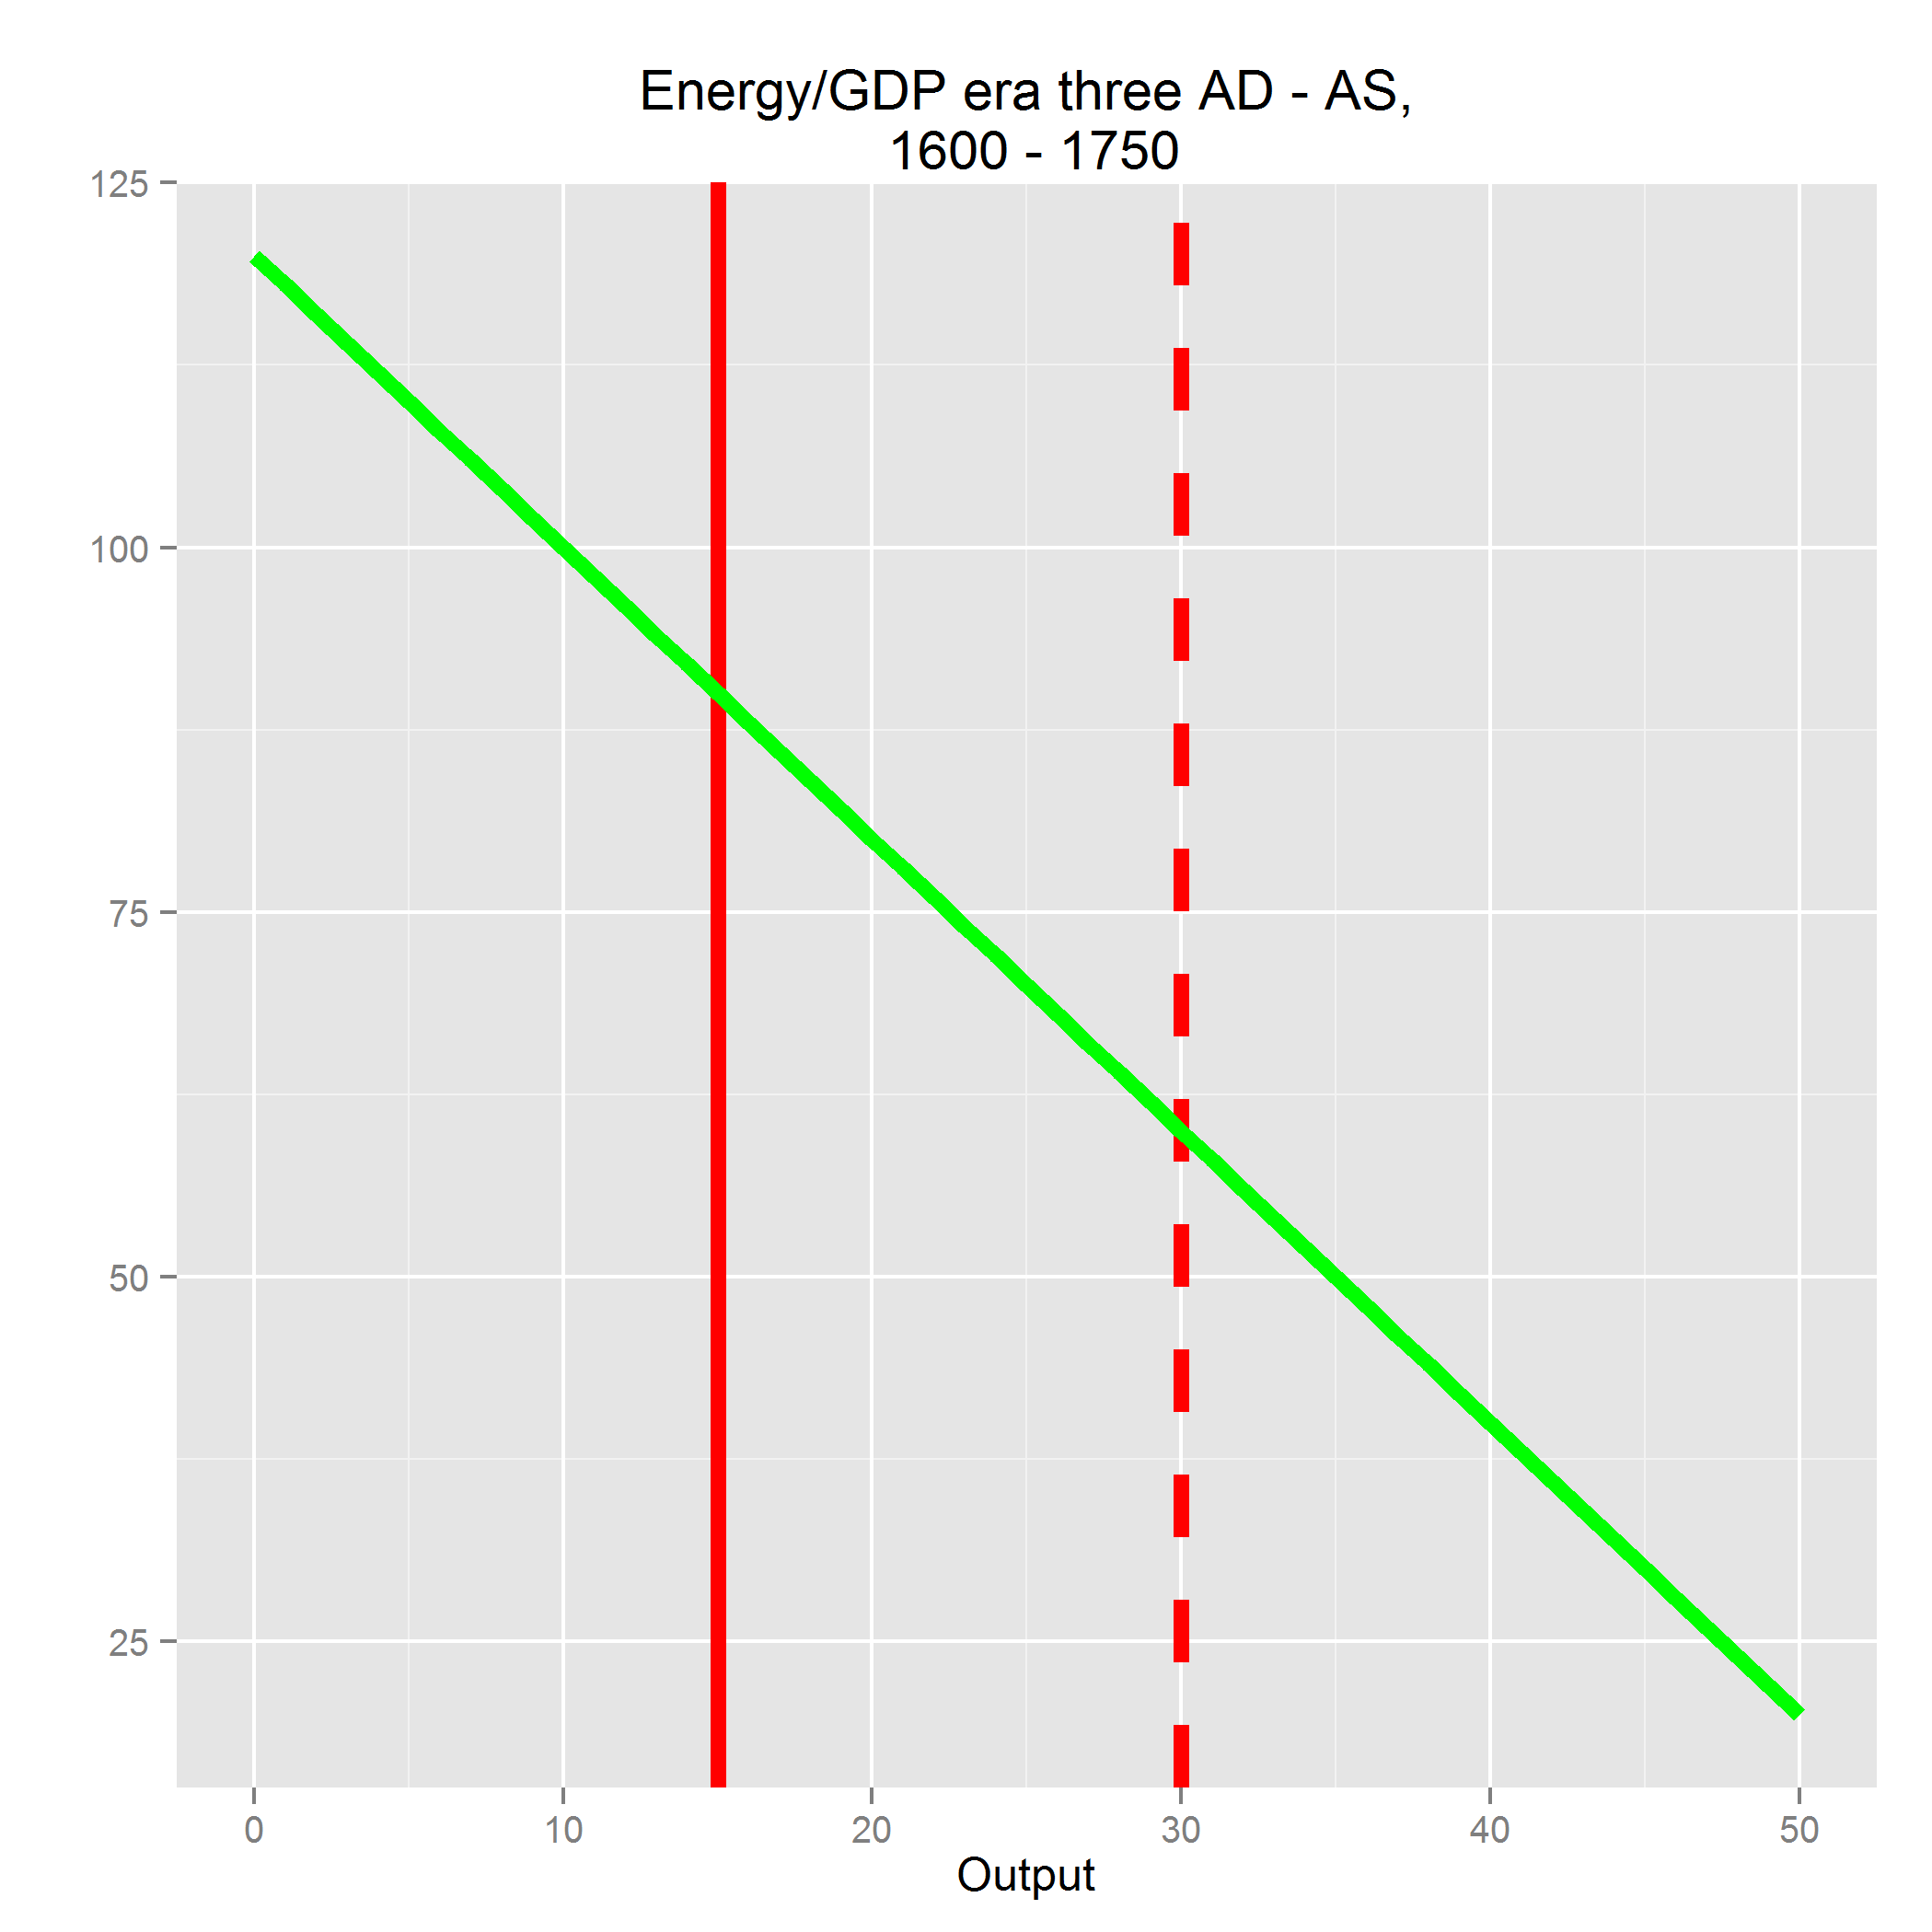
\includegraphics[width=0.25\textwidth]{era3}}
		\mbox{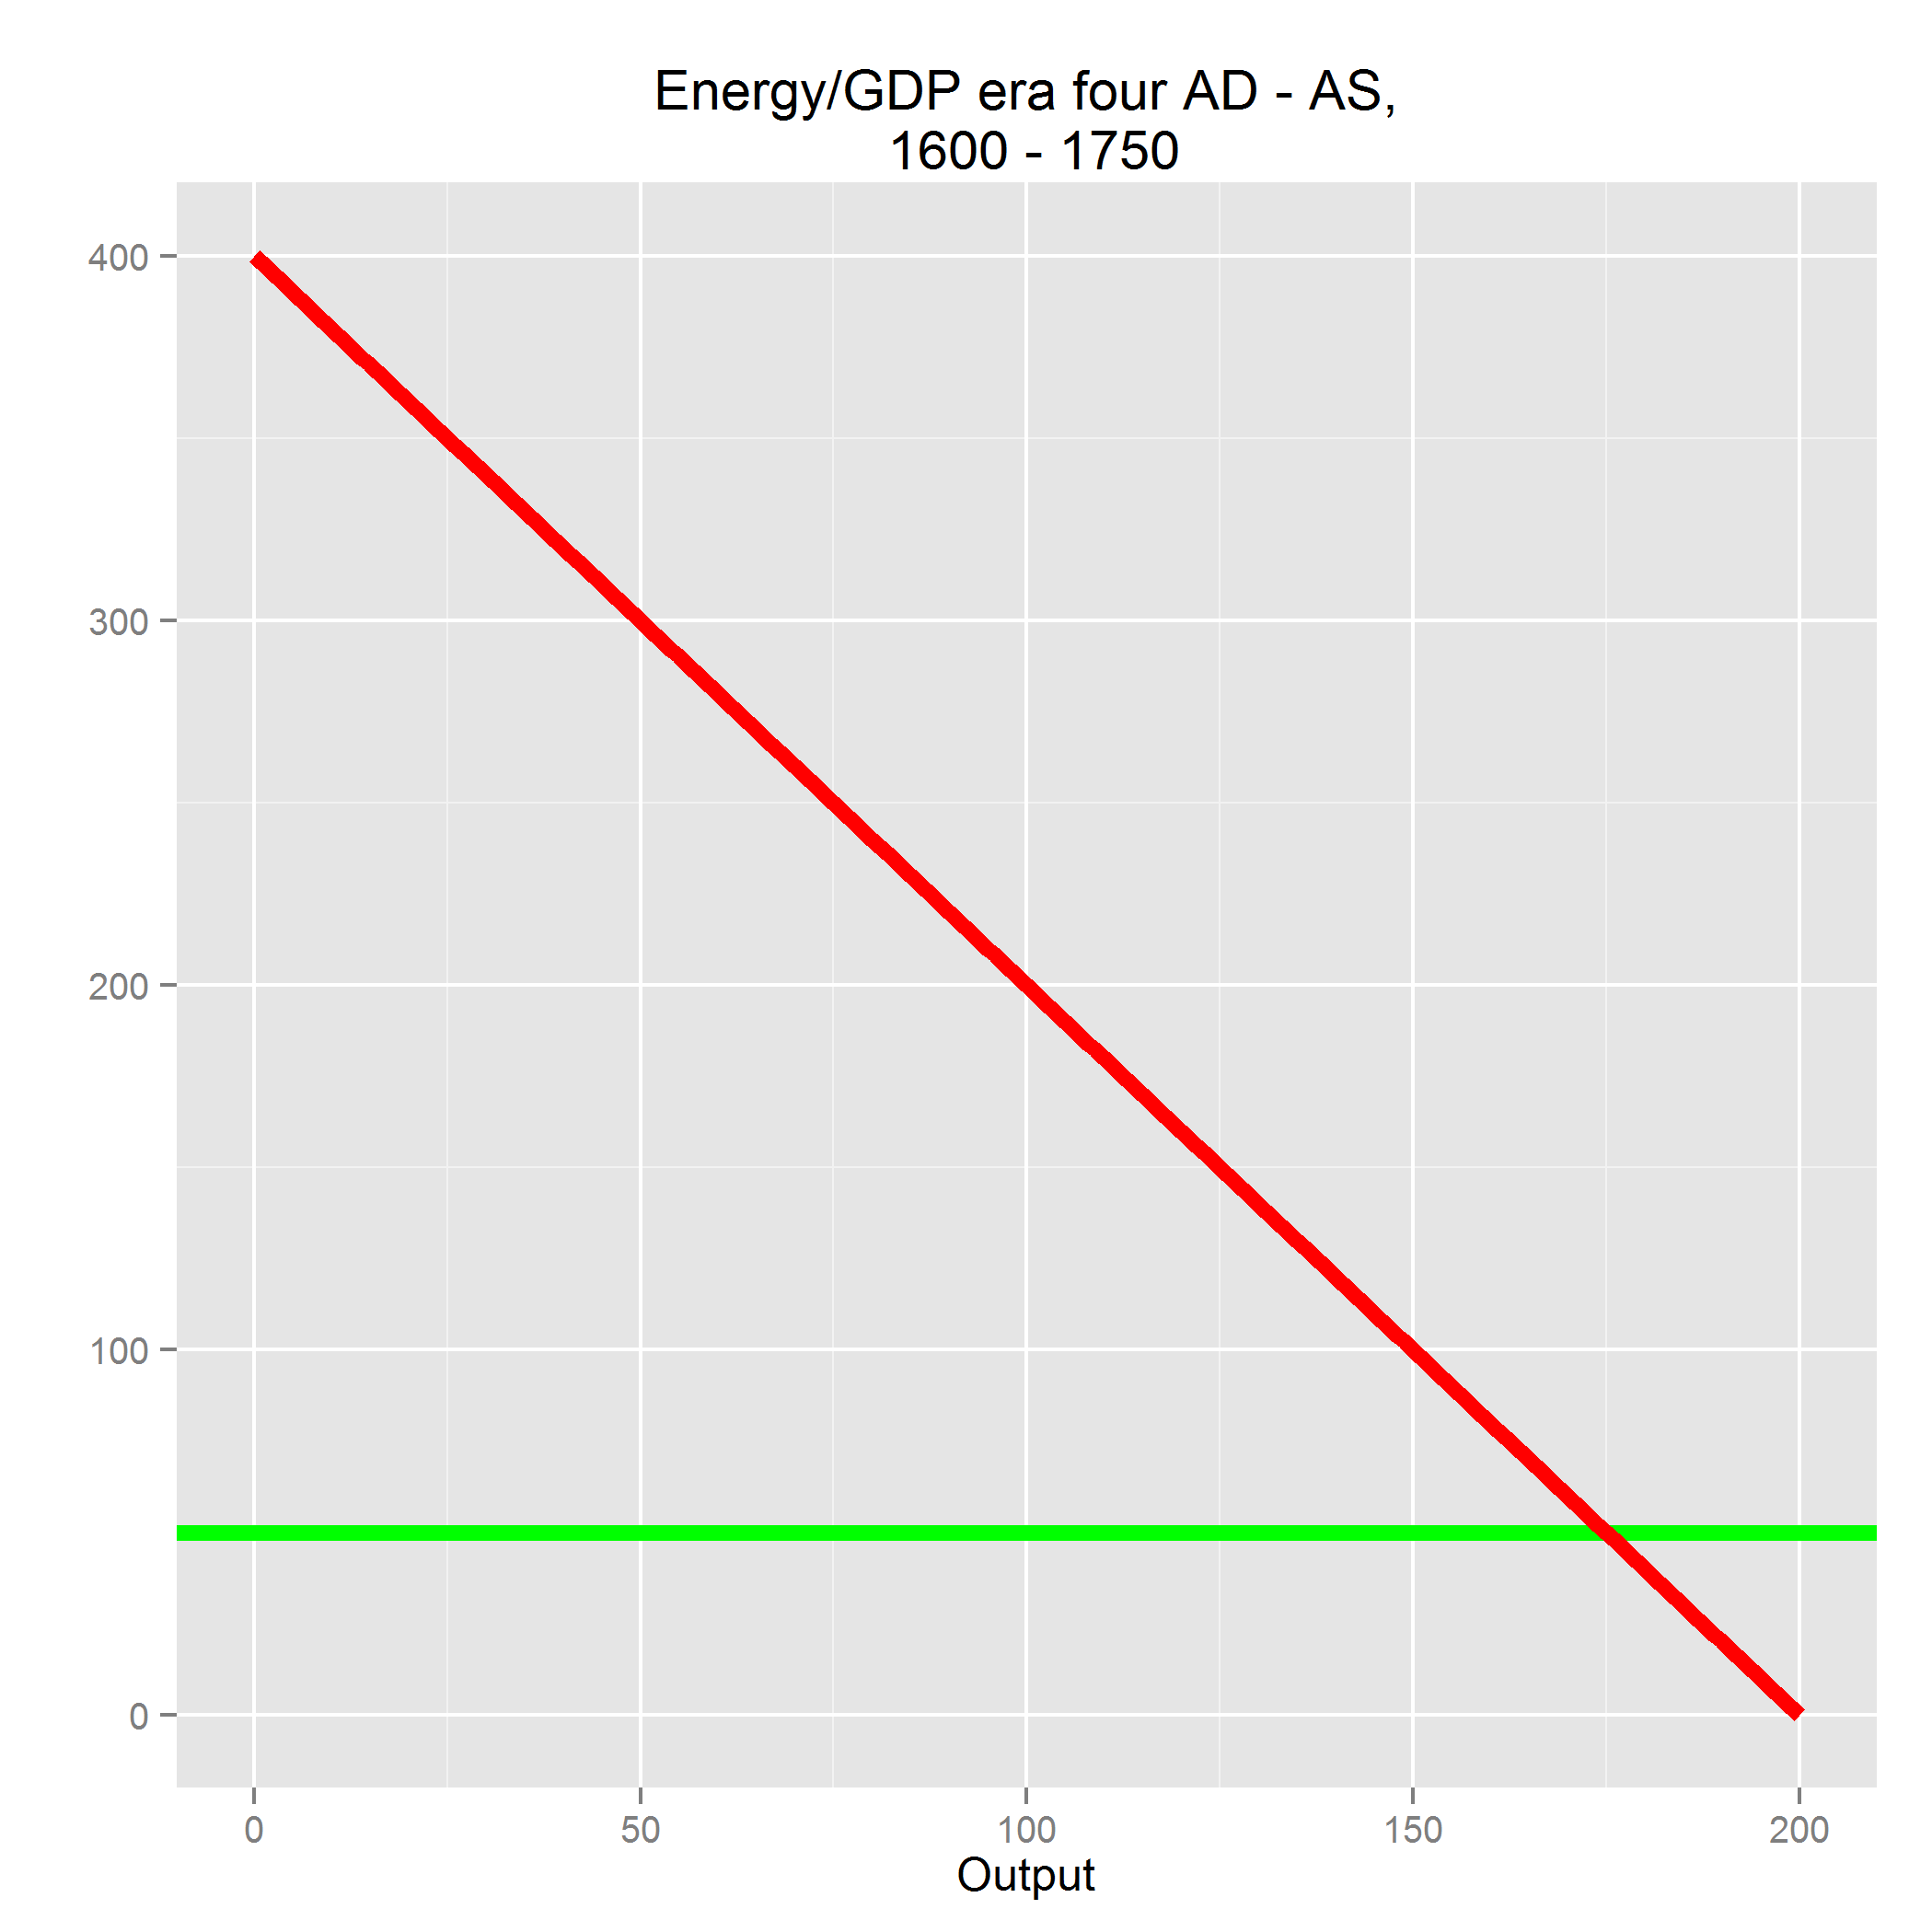
\includegraphics[width=0.25\textwidth]{era4}}				
		}
		\end{figure}

\begin{figure}[p!]
		\caption{Desagulier manuscript}
		\label{fig:desagulier}		
		\center
%		\mbox{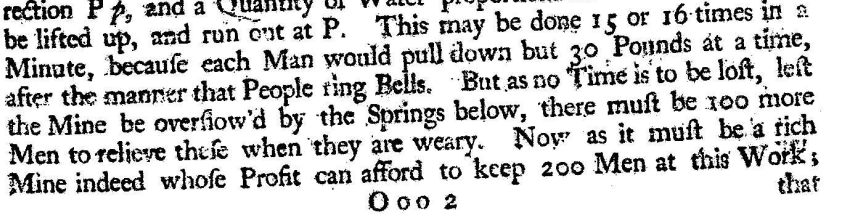
\includegraphics[width=0.95\textwidth]{desagulier1}}\\
%		\mbox{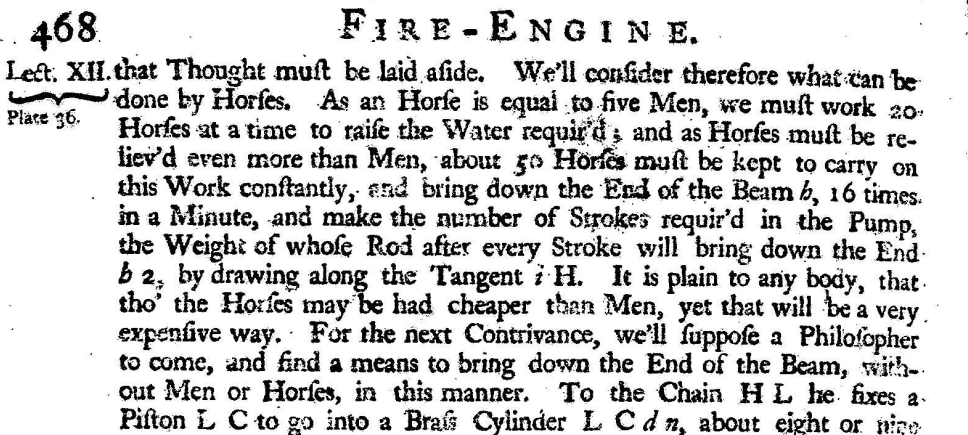
\includegraphics[width=0.95\textwidth]{desagulier2}}
		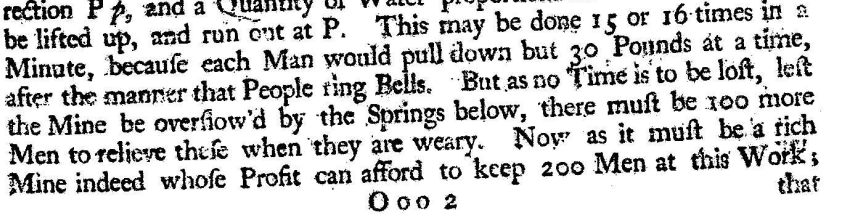
\includegraphics[width=0.95\textwidth]{desagulier1}\\
		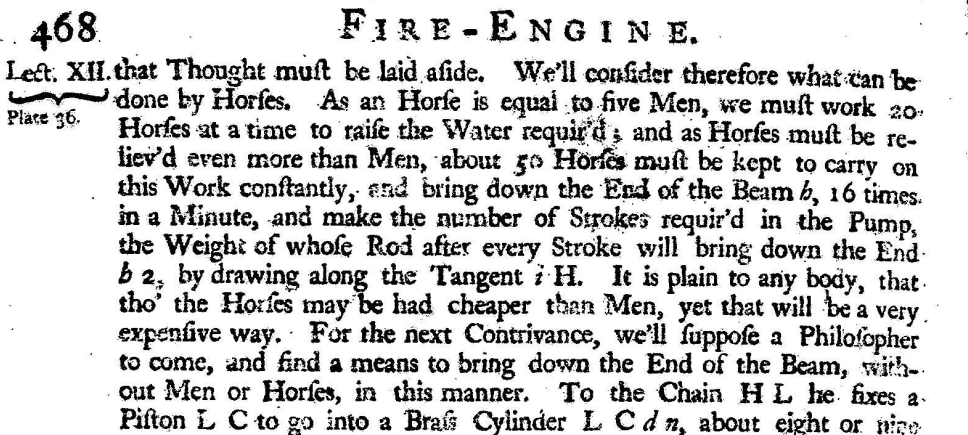
\includegraphics[width=1.05\textwidth]{desagulier2}
%		}
\end{figure}

\begin{figure}[p!]
\center
\caption{Real wage to energy ratios\\\textit{Source:} Robert Allen (2009)}
\label{fig:wage-energy}
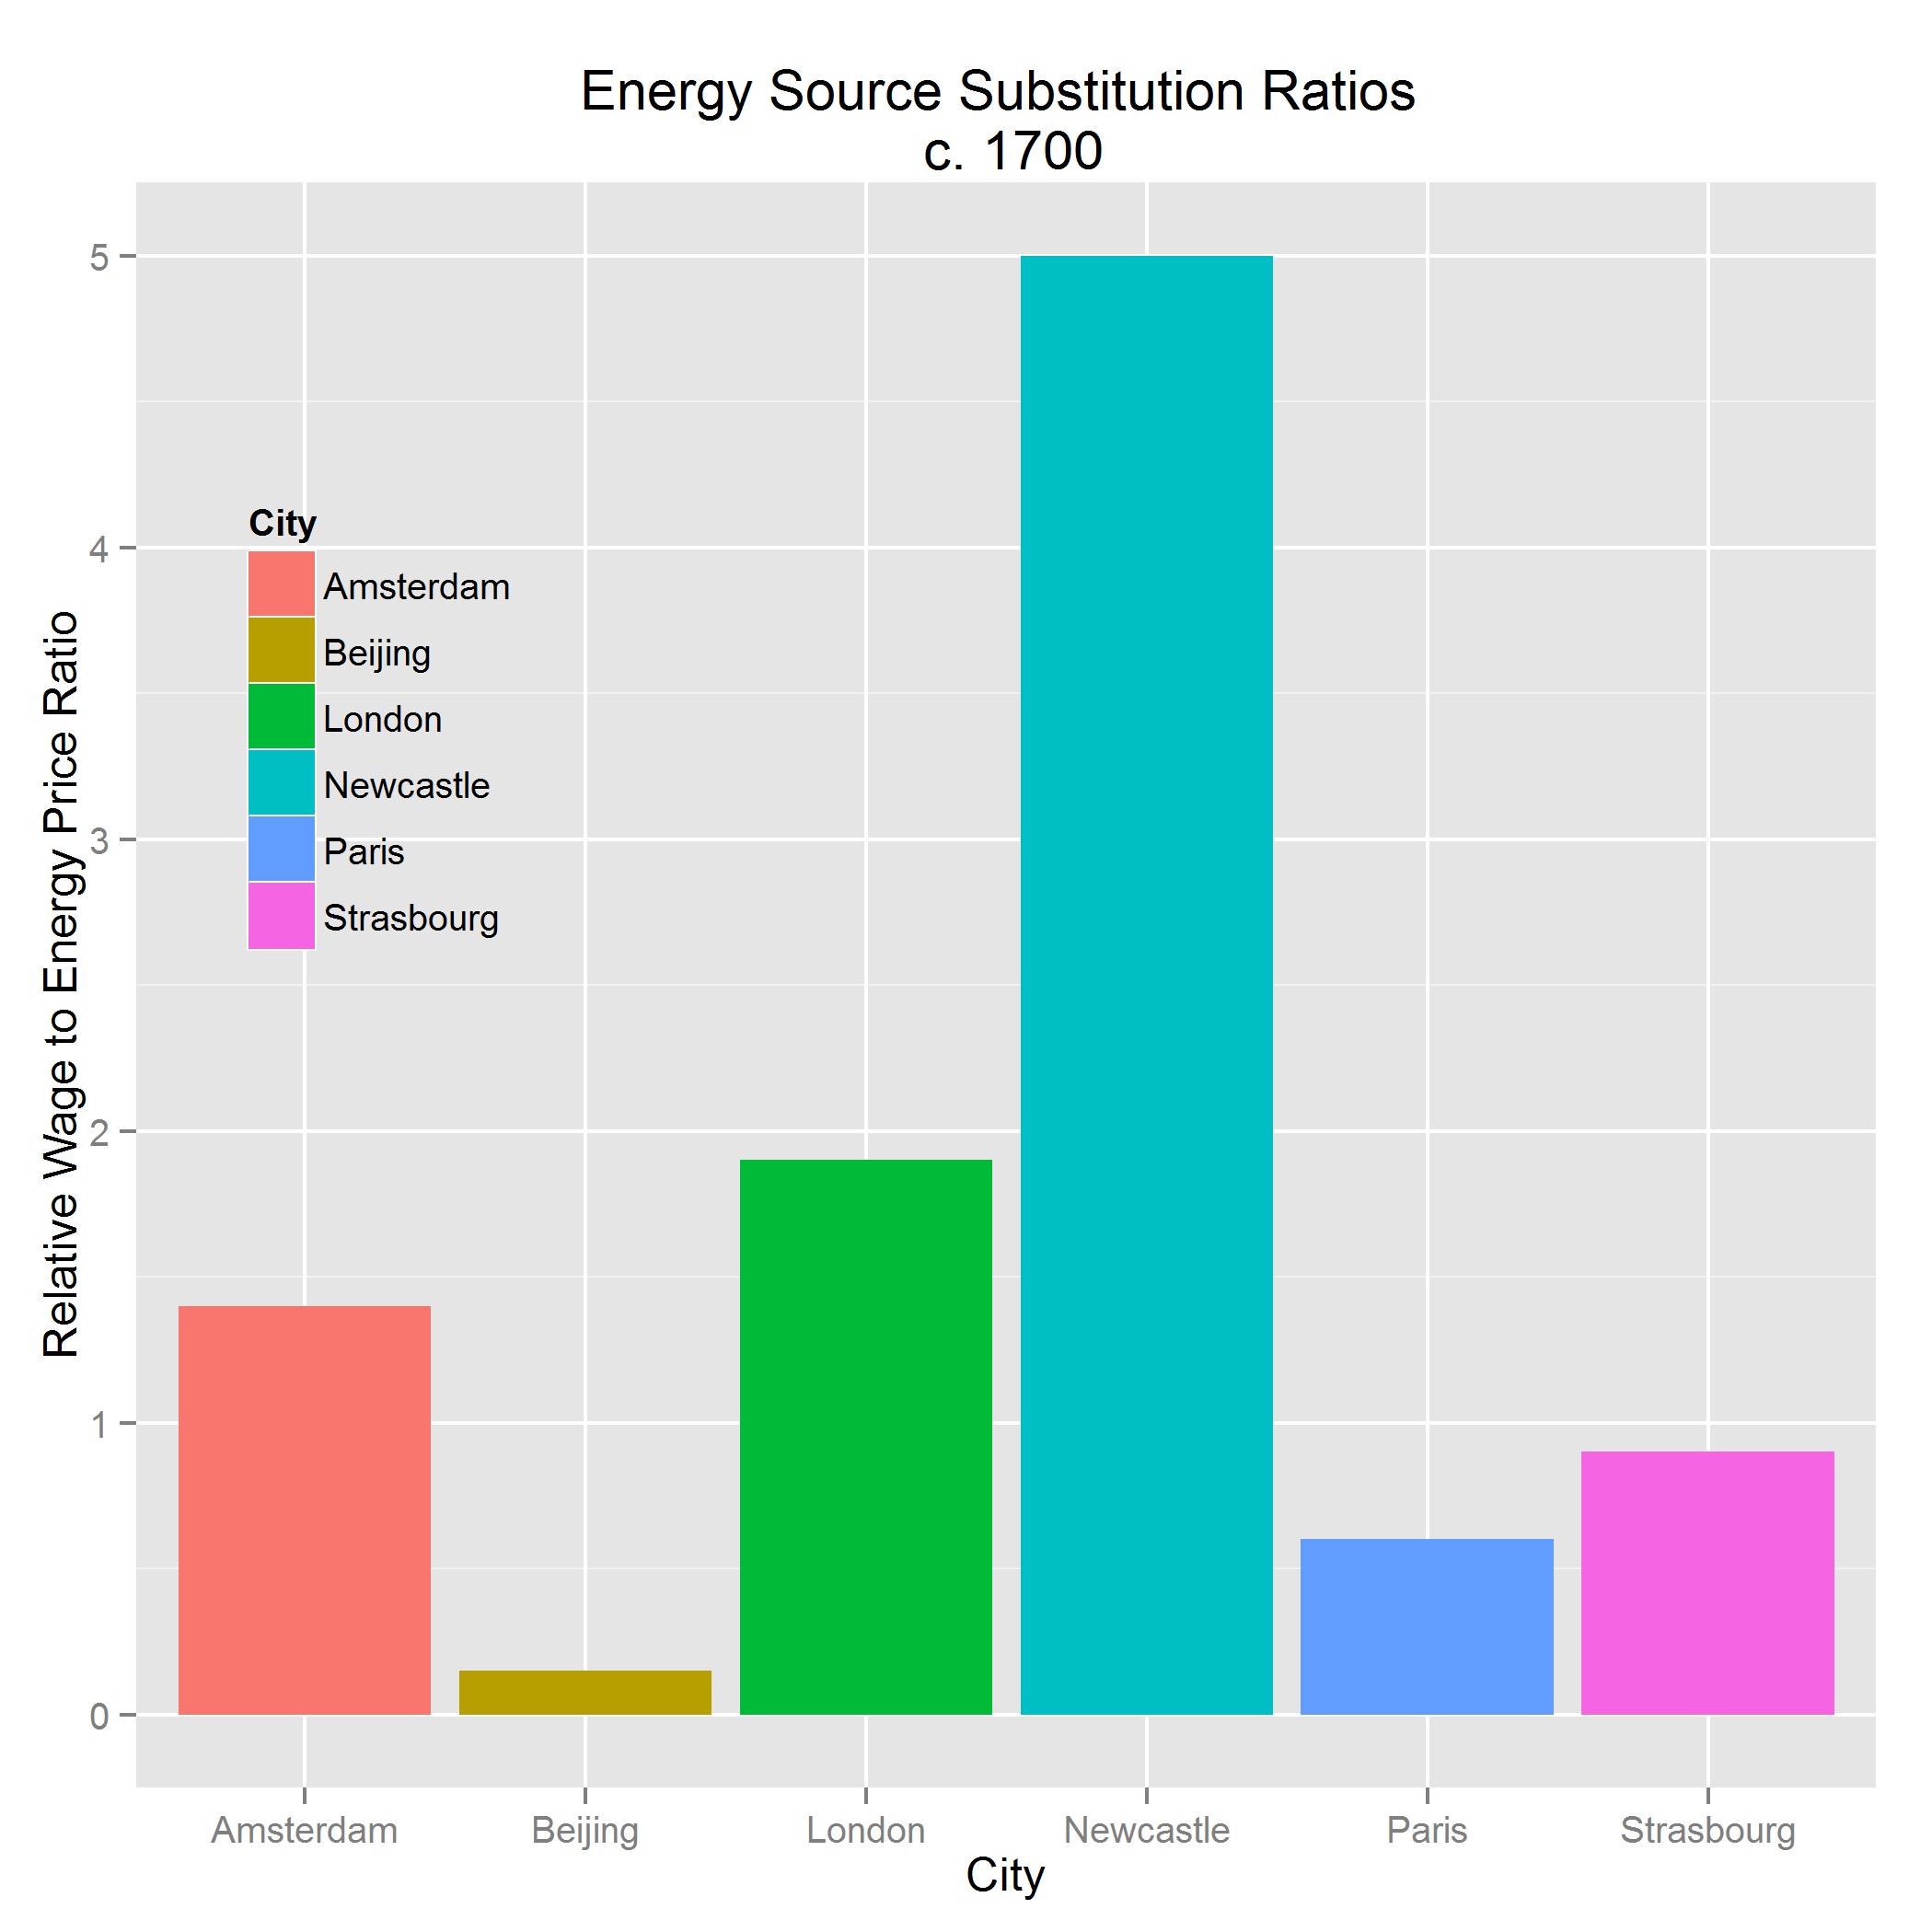
\includegraphics[width=0.9\textwidth]{wage-energy.png}
\end{figure}

\begin{figure}[p!]
\center
\caption{Standardized English energy intensity of GDP}
\label{fig:energyIntensity}
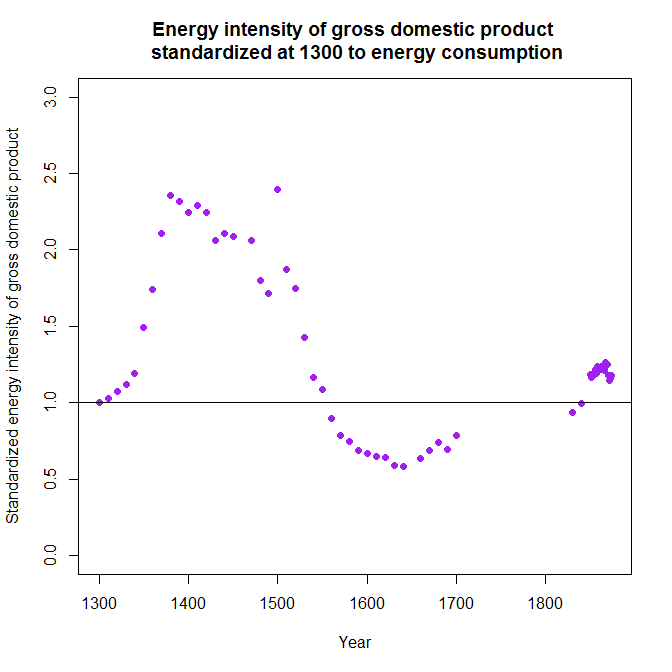
\includegraphics[width=0.9\textwidth]{energyIntensity}
\end{figure}

\begin{figure}[p!]
\center
\caption{Log of GDP, with structural breaks}
\label{fig:gbpgdplog.png}
\includegraphics[width=0.9\textwidth]{gbpgdplog.png}
\end{figure}
\end{comment}
\newpage

\section{Equations}

		\begin{equation}
		\label{eq:mrp}
		\frac{\text{Marginal Revenue Product}_{\text{ organic energy joule}}}{\text{Price}_{\text{ organic energy joule}}} = \frac{\text{Marginal Revenue Product}_{\text{ fossil energy joule}}}{\text{Price}_{\text{ fossil energy joule}}}
		\end{equation}
		\myequations{Microeconomic theory - marginal revenue product} 
		
%granger tests over at least two regimes

\section{Appendix A. Detailed Granger test output} 
\label{app:Appendix A}

\section{Appendix B. Time series analyses}
\label{app:Appendix B}

\begin{comment}
\section{Appendix C. Future research}
survey on institutions/culture\\
empirical tests of institutional/cultural events\\
population curves\\
\label{app:Appendix C}
\end{comment}


\begin{comment}

\begin{verbatim}
> grangertest(per1eng ~ per1gdp,n)
Granger causality test

Model 1: per1eng ~ Lags(per1eng, 1:1) + Lags(per1gdp, 1:1)
Model 2: per1eng ~ Lags(per1eng, 1:1)
  Res.Df Df      F  Pr(>F)  
1     16                    
2     17 -1 8.3703 0.01059 *
---
Signif. codes:  0 �***' 0.001 �**' 0.01 �*' 0.05 �.' 0.1 � ' 1 
 grangertest(per1gdp ~ per1eng,n)
Granger causality test

Model 1: per1gdp ~ Lags(per1gdp, 1:1) + Lags(per1eng, 1:1)
Model 2: per1gdp ~ Lags(per1gdp, 1:1)
  Res.Df Df      F    Pr(>F)    
1     16                        
2     17 -1 21.772 0.0002582 ***
---
Signif. codes:  0 '***' 0.001 '**' 0.01 '*' 0.05 '.' 0.1 ' ' 1 
> grangertest(per2eng ~ per2gdp,n)
Granger causality test

Model 1: per2eng ~ Lags(per2eng, 1:1) + Lags(per2gdp, 1:1)
Model 2: per2eng ~ Lags(per2eng, 1:1)
  Res.Df Df      F Pr(>F)
1      7                 
2      8 -1 2.0643 0.1939
> grangertest(per2gdp ~ per2eng,n)
Granger causality test

Model 1: per2gdp ~ Lags(per2gdp, 1:1) + Lags(per2eng, 1:1)
Model 2: per2gdp ~ Lags(per2gdp, 1:1)
  Res.Df Df      F Pr(>F)
1      7                 
2      8 -1 0.2808 0.6126
> grangertest(per3eng ~ per3gdp,n)
Granger causality test

Model 1: per3eng ~ Lags(per3eng, 1:1) + Lags(per3gdp, 1:1)
Model 2: per3eng ~ Lags(per3eng, 1:1)
  Res.Df Df      F Pr(>F)
1      6                 
2      7 -1 1.0136 0.3529
> grangertest(per3gdp ~ per3eng,n)
Granger causality test

Model 1: per3gdp ~ Lags(per3gdp, 1:1) + Lags(per3eng, 1:1)
Model 2: per3gdp ~ Lags(per3gdp, 1:1)
  Res.Df Df      F Pr(>F)
1      6                 
2      7 -1 0.4703 0.5185
> grangertest(per4eng ~ per4gdp,n)
Granger causality test

Model 1: per4eng ~ Lags(per4eng, 1:1) + Lags(per4gdp, 1:1)
Model 2: per4eng ~ Lags(per4eng, 1:1)
  Res.Df Df      F   Pr(>F)   
1     22                      
2     23 -1 11.735 0.002418 **
---
Signif. codes:  0 '***' 0.001 '**' 0.01 '*' 0.05 '.' 0.1 ' ' 1 
> grangertest(per4gdp ~ per4eng,n)
Granger causality test

Model 1: per4gdp ~ Lags(per4gdp, 1:1) + Lags(per4eng, 1:1)
Model 2: per4gdp ~ Lags(per4gdp, 1:1)
  Res.Df Df      F Pr(>F)
1     22                 
2     23 -1 2.7737   0.11

\end{verbatim}
\end{comment}

\end{document}
\section{end}

\section{Defence proposal below here}
\newpage
			
	\section{Table of Contents}
	\tableofcontents
	\listoffigures
	\listoftables
	
	\newpage
	

	\section{The Research Question}
	
	The origins and causes of the English Industrial Revolution remain among economic history's most contested puzzles.  This slowly evolving revolution was likely the most important event in economic history since the \gls{neorev} approximately 10,000 years ago, and eclipses even that unquestionably cataclysmic transition in economic importance as measured by growth in per capita income.  Table \ref{tbl:gdpcapita} shows the growth in world per capita real income between CE 1 and 1900. \footnote{Data from Maddison 2007 \cite{maddison_world_2007}} Yet, even this primary outcome of the Industrial Revolution remains contested.
	
	In the first 17 centuries of the Current Era per capita output increased by about 32 percent, surely still hewing closely to subsistence.  By stark contrast, in the two hundred years between 1700 and 1900 world average per capita output increased by  over 100 percent.  If one considers the very narrow population base to which the increased income actually inured (about 15 percent of the 1900 world population, measured by nation-state, produced about 40 percent of world GDP), this is a remarkable outcome. The richest country in 1900, the United Kingdom, enjoyed per capita income of about 4,500 \gls{gkusd}, over three times the world average.
	
		\begin{table}[h!]
		\centering

%		\begin{adjustwidth}{-0.75in}{}

		\caption[World GDP per capita]{This table shows the growth of world GDP per capita in two periods covering almost two millennia. Maddsion's data, author's calculations. Dollars in 1900 Geary-Khamis International (US) Dollars}\label{tbl:gdpcapita}
		
		\begin{tabular}{lrr}
		\toprule
		Benchmark&GDP per capita,&Percent Increase\\
		Year&1990 G-K\$& from prior benchmark\\
		\midrule \midrule
		CE 1&467&-\\
		1700&615&31.7\%\\
		1900&1,261&105.0\%\\
		\bottomrule

		\end{tabular}
%		\end{adjustwidth}
		\end{table}
	
	In some respects, the English consumers and inventors between the reigns of \gls{lizIreign} and \gls{vicreign} forged a Faustian bargain with the future to achieve this miracle.  They almost surely did so unknowingly by unleashing a historically unprecedented positive feedback cycle of demand and production that has now lasted for 400 years; this event thus has the characteristic of an emergent macroeconomic effect.  %History also inserts great economic inequalities, instabilities and conflicts, environmental damages, and other existential threats into this record of unprecedented growth in incomes, surplus, and, thus, wealth for wide swaths of humanity.
	
	What happened?  How did it happen?  Why did it happen first in England when it did and nowhere else in accumulated history?  Why has it not regressed, as every known preceding surge in per capita income has done?  
	
	How should our understanding of this Revolution inform our understanding of economic development in the nation-states and global economy that followed England -- that is, how did the Revolution evolve and spread?  What can we learn about future economic development and growth?
	
	And very specifically, what role did effectively unconstrained rates of \gls{energy} play in the Revolution? What social and institutional changes help account for this ``miracle invention" by which the English for the first time in history, and uniquely at the beginning, ``escaped the constraints of an advanced organic society?" \footnote{Wrigley 2010, p. 239 \cite{wrigley_energy_2010}} In turn, what social and institutional changes did this revolution cause in England and the other economies which followed in her path?
	
	I consider whether this discovery--\textit{the ability to convert virtually unlimited energy to output through the macro-invention of industrial-scale machine-capitalism} \footnote{Eckel \textit{Coal, Iron, War}, 1921  \cite{eckel_coal_1921}}---is the real, although in significant senses accidental, invention of the Revolution.  If so, we must consider this history seriously as we gaze into the physical and economic future of our species and planet.

		\subsection{What is the Study About?}
		
			\subsubsection{Nature and significance}
			This study explores the role of energy consumption in \gls{growth} and development.  The research question arises as one views long-period time-series of both per capita output and per capita energy consumption.  Both can be best described visually as super-exponential growth curves; thus, it is natural to ask how they are related.  The characteristic shape is seen in Figure \ref{fig:road}.\footnote{Economist Magazine, December 23, 1999  \cite{_road_1999}}
			
			\begin{figure}
			\centering
			\caption[Road to riches hockey stick]{From a 1999 Economist magazine article, based on the Angus Maddison data, illustrating the ``hockey stick'' effect of per capita GDP growth in Europe. Usefully annotated with historical events}\label{fig:road}
			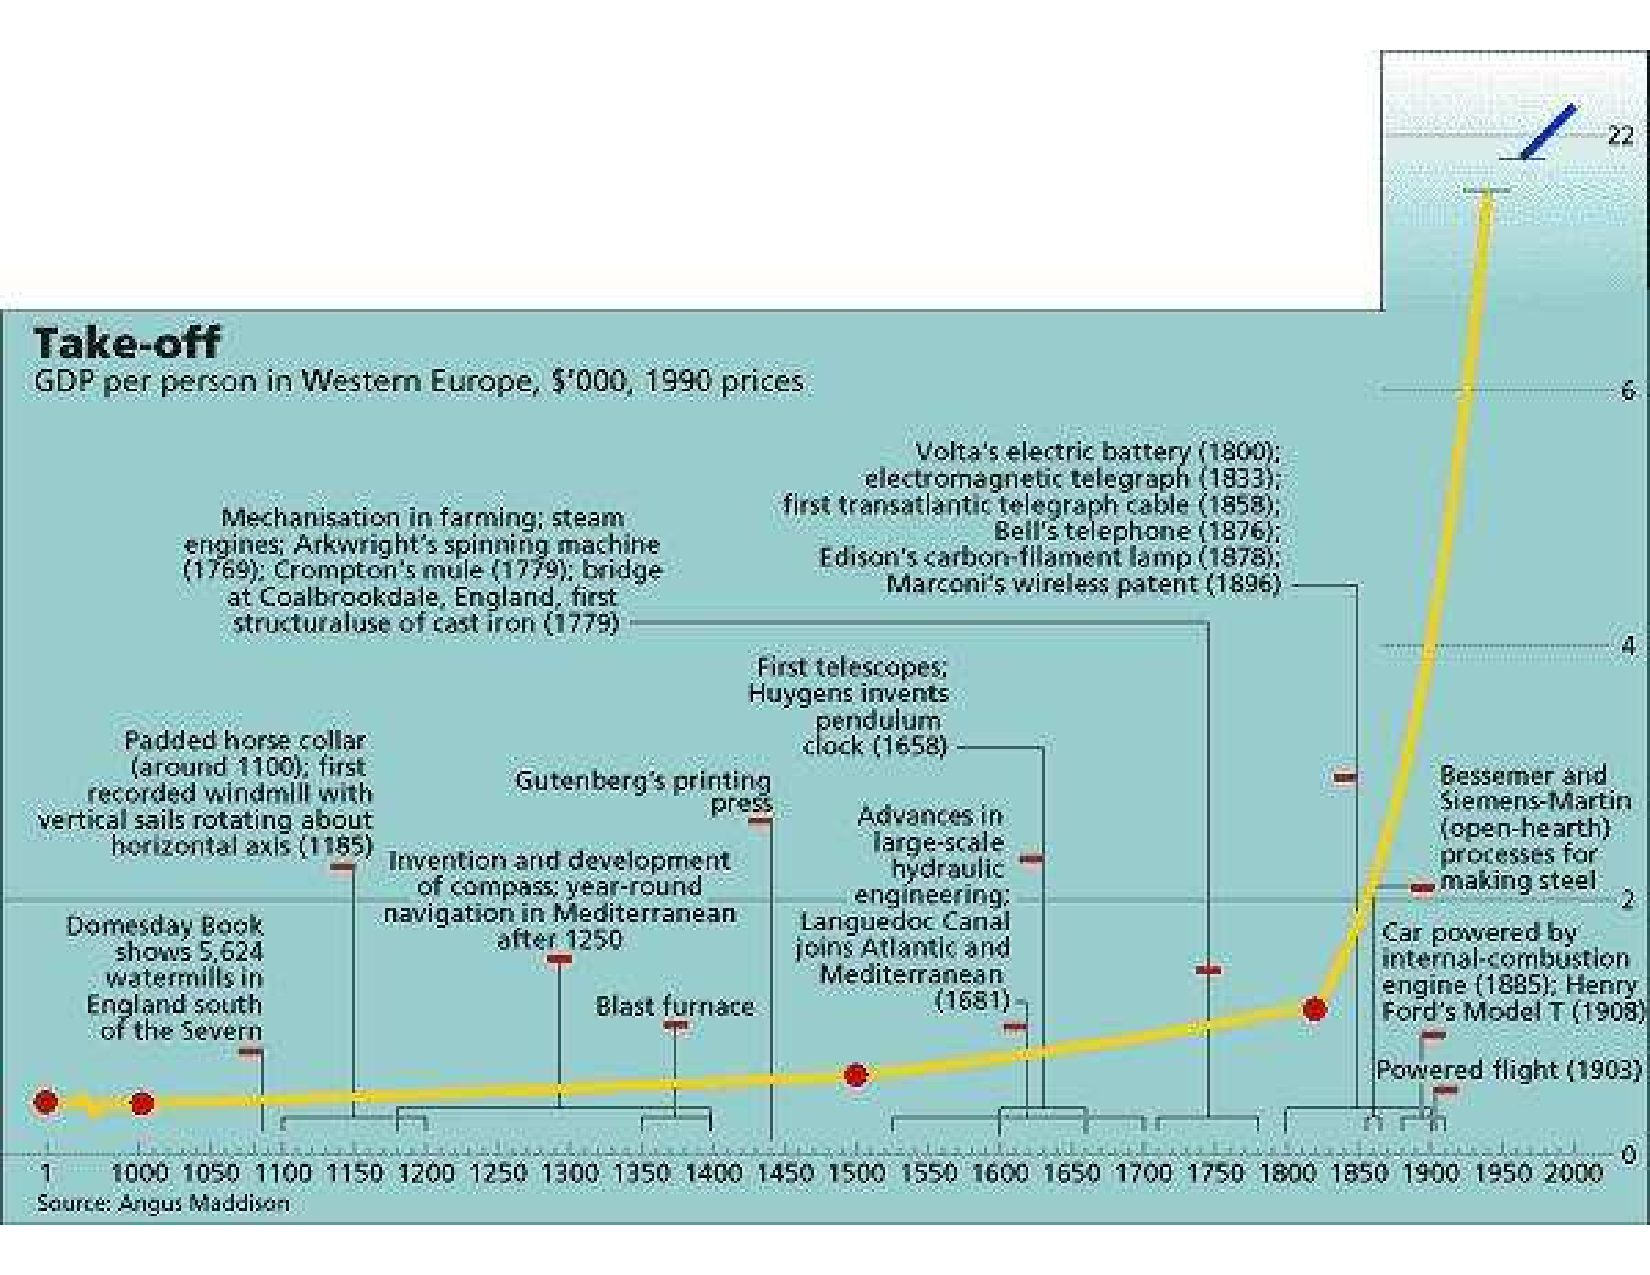
\includegraphics[width=0.8\textwidth]{../images/roadtoriches.pdf}
			\end{figure}
		
			A word on the title: Sir Arthur A. Lewis in his iconic 1954 ``Economic Development with unlimited supplies of labour'' \footnote{Lewis, 1954.\cite{lewis_economic_1954}} develops as a central theme that, in underdeveloped economies, labour will be used even if its marginal product is zero due to its relative abundance.
			
			I can construct similar examples in modern energy use; suppose I left the computer on which I am composing this unattended but on for several hours before writing this paragraph. It is not clear what the marginal product of that unattended energy consumption is: The computer did no writing or editing while I was absent. If I were writing by quill pen and candlelight, I would likely not have left the candle burning unattended due to fire risks and the high per lumen cost of medieval candles. The abundance of modern energy changes the expected marginal cost/marginal benefit equation.
			
			Another way to think about modern energy consumption is that the ratio of mineral energy available for whatever task, be it commodity manufacturing, service provision of various kinds including transportation, or writing a dissertation, is virtually unconstrained relative to the amount of the very largest amount of human energy I could possibly marshal for any of those tasks.
			
			So the title contextualizes the way in which I view modern energy consumption, and emphasizes how uniquely important the great English invention was.
			
			\subsubsection{Contributions of the study}
			\begin{enumerate}
			\item I clarify the historical explanation of this Revolution.  The explanation has fragmented over several economic generations into several ``camps" from which I hope to abstract what is both necessary and sufficient to explain the magical event. The story is complex, enriched with feed-back mechanisms, and clearly not mono-causal in the choices of supporting historical events.
			
			One can view the range of prior explanations of the English Industrial Revolution as a continuum from purely cultural to purely thermodynamic, with religious, cultural, social, institutional, technological, and geographical explanations arrayed along the line. By far, the most common explanations are weighted toward some form of English cultural exceptionalism. 
			
			\label{par:deirdre} Perhaps the most eloquent of this class is the recent series of books by Deirde McCloskey currently being published under the banner of the ``Bourgeois Era.''  Professor McCloskey details (in a promised six volumes) the great cultural changes that surrounded the English Industrial Revolution.  The series describes processes which are the antithesis of Marxian historical materialism. While there are many compelling stories in this history, this paper counters her thesis with a conviction that the actual story is, in fact and on the evidence, primarily a materialist story which caused and was supported by the evolving cultural and institutional environments. \footnote{The series currently consists of two published volumes, ``The Bourgeois Virtues'' (2007), and ``Bourgeois Dignity'' (2010) \cite{mccloskey_bourgeois_2010}}
			
			
			\item I propose a new definition of the English Industrial Revolution: a historically unique development that enabled the English macroeconomy to consume a virtually unconstrained amount of energy, and thus to escape any practical supply side limitation on output.  For perhaps the first time in history demand, not supply, became the limit of output; output growth exceeded population growth for an extended period of time.  Unprecedented growth of both macroeconomic productivity and \gls{surplus} accumulation became the new normal.
			
			\item Further, I explore my intuitions with the most analytically useful analysis I am aware of for this kind of problem.  Specifically, I  use the methodology of the so-called \gls{copenhagen} to investigate and attempt to explain the relationships and dynamics among energy consumption rates, output growth, and population growth. The method allows admitting exogenous events, so that if, for example, a statistical structural break appears in the data starting near the time of Gutenberg's invention, one can both recognize that in the model in a control sense and hypothesize that it was an important event. While the historically constructed series I use can surely be problematic, in a sense testing them with rigorous statistics could possibly highlight weaknesses in the construction methods.
			
			The method is capable of decomposing feedback loops into both short-run and long-run components.  To my knowledge, this decomposition method has never been attempted over long historical-period data sets.
			
			\item I apply the empirical methodology to two relatively new long-period histories of English energy consumption. One is from Roger Fouquet, \footnote{Fouquet's new study on English energy \cite{fouquet_heat_2008}} and one from Paul Warde. \footnote{Energy consumption from Warde's 2007 work. \cite{warde_energy_2007}} My strategy is to empirically test both inputs and compare the results both economically and statistically.
			
			\item As a future research agenda, 
			
			\begin{enumerate}
			
			\item I will extend this methodology to examine other economies in phases of significant growth; clearly the United States and China should be included, but any economy with sufficient historical data is a potential target. \label{par:china}
			
			\item I will use the empirical methods to decompose global growth over the period with available meaningful data.  
			
			\item Finally, I may consider an energy-based theory of income, growth, and wealth, and contrast that with extant micro-economic marginal productivity based theories including "new growth" New-Keynesian theories. If energy consumption is proven foundational to economic growth, then a measure of \gls{surplus} as energy consumption above \gls{bio} \footnote{Brad DeLong 1998. DeLong discusses GDP and population estimates, and uses this evocative term. \cite{delong_estimates_1998}} may prove interesting and useful.
			\end{enumerate}
			\end{enumerate}

		\subsection{Statement of the Research Question and Main Hypothesis}
		The research question asks how English energy consumption and economic output are structurally related, considering population levels, over a long period preceding and spanning the English Industrial Revolution.
		
		My main hypothesis is that learning to consume unconstrained energy was responsible, at least in the statistically causal sense, for the massive increases in per capita output first demonstrated in the English Industrial Revolution. Refer to Figure \ref{fig:road} and Table \ref{tbl:gdpcapitauk} for historical English per capita GDP growth.\footnote{Data from Maddison 2007 \cite{maddison_world_2007}}
		
		\begin{table} \centering
		\caption[UK GDP per capita]{This table shows the growth of English GDP per capita in two periods covering almost two millennia. Maddsion's data, author's calculations. Dollars in 1900 Geary-Khamis International (US) Dollars}\label{tbl:gdpcapitauk}.
				
		\begin{tabular}{lrr}
		\toprule
		Benchmark&UK GDP per capita,&Percent Increase\\
		Year&1990 G-K\$& from prior benchmark\\
		\midrule \midrule
		CE 1&400&-\\
		1700&1,250&212.5\%\\
		1900&4,492&259.4\%\\
		\bottomrule

		\end{tabular}
%		\end{adjustwidth}
		\end{table}
		
		Thus, an understanding of that event is crucial to understanding \gls{growth}.


		\subsection{Subsidiary Hypotheses}
		\begin{enumerate}
		\item While the primary and clear discovery of the English Industrial Revolution was the ability to consume unlimited energy at the level of the macro economy, there are a series of necessary social and institutional precursors. 
		
		These are in dispute, but I focus on identifying those that contributed to the incentives and skills of consuming unlimited energy. My initial candidates are the rise of consumer demand including (though at a later time) the export orientation of the English economy, and the accelerated accumulation and spread of knowledge after Gutenberg's \footnote{Johannes Gutenberg, 1398 - 1468, widely credited with inventing a printing press using mechanical moveable type} printing invention.
		
		Following Cottrell \footnote{W. F. Cottrell 1955 \cite{cottrell_energy_1955}} (and Karl Marx), there should also be testable hypotheses on the energy revolution causing social and institutional changes. This is an area for future research.
		
		\item While England clearly led, the revolution spread fairly quickly. I hypothesize that the structural dynamics of the early followers were similar to those of England.  Via the framework I am developing, this should be a testable hypothesis in future research.
		

		
		\item I further hypothesize that the rate of energy consumption is a much better predictor of \gls{surplus} than any other factor including ``capital'' and ``technical progress,'' as they would enter a common specification of the Solow macro production function.
		\end{enumerate}


  		\subsection{Limitations and Delimitations}
		
		In this proposal, the focus is on the English experience; I do extend the model to a global economy by testing specifications which admit English exports as support for growth in overall demand. In the research for this proposal, country comparisons arise and I reference them. As I continue this work, I will extend the methods to other key economies as described on page \pageref{par:china}.

		\subsubsection{Limitations}
		The primary limitation in the study is the accuracy of the data series since they are historically constructed by various economic historians.  I will evaluate several sources for the data and attempt to make a logical choice of which series I will use.  As questions arise on the accuracy, my considered response is ``what choice do we have?"  We should let the data tell us whether the model(s) using the series are credible statistically. Thus, doing the econometric analysis in this way may be peripherally useful to the historians who have been compiling this data, as it will suggest the validity of the data.
		
		\subsubsection{Delimitations}
		The primary delimitation that I have imposed is to use only three time series as core variables in the proposed study; Gross Domestic Product (GDP), energy consumption, and population are treated as endogenous variables. I will allow historical events suggested by structural breaks in these endogenous series to enter the model.  Depending on model fits, I may consider adding other theoretically justifiable series, for example, energy prices. This parsimonious ``simple to complex'' approach is the preferred methodology of the \gls{copenhagen}.
		
		I prefer to use Bayesian inference rather than classical methods for it's superior statistical characteristics. However, the applied methodology I need to deploy is not yet up to the challenge, so I will limit this study to classical inference.

		
	\section{Literature Review}
	There are two main bodies of literature that bear on my topic.  The first deals with the historical causes of the English Industrial Revolution, and the subsequent histories of the other countries which bear on their path to modern economic growth.
	
	The second body of literature deals with the econometric analysis of energy and modern economic growth.
	
	This study will both deal with the intersection of these bodies of literature, and extend them in the following ways:
	\begin{enumerate}
	\item Use econometric methods to fully describe the structural dynamics, both long- and short-run, relating economic growth and energy consumption.
	\item Identify the most important historical-institutional changes that led to modern economic growth as first experienced in the English Industrial Revolution.
	\item Since the prime cause of the English Industrial Revolution remains under debate, I will attempt to add to the debate based on the evidence.
	\end{enumerate}
	
	\subsection{Contributions of the core literature}

	\paragraph{Primarily cultural explanations of the English Industrial Revolution -- the English cultural exceptionalists.} In line with my metaphor of a continuum of primary reasons to explain why the Industrial Revolution was English and happened in the $18^{th}$ century, I first describe some of the more prominent cultural or institutional primacy authors. Note that almost all historians who approach this problem end up with multi-causal explanations, so this categorization is based on my judgement. 
	
	Deirdre McCloskey, who I referenced earlier, provides an acutely observed and detailed history of the cultural, social, and institutional changes that contributed to the Industrial Revolution. As is common among these scholars, coal gets a mention. In fact it gets a full chapter (22) in McCloskey's ``Bourgeois Dignity'', \footnote{McCloskey 2010 \cite{mccloskey_bourgeois_2010}} but is only one of very many factors (and chapters -- a total of 46) for McCloskey.
	
	David Landes, with his ``The Unbound Prometheus'', \footnote{Landes 1969 \cite{landes_unbound_1969}} became the mainstream doyen of recent documenters of the Industrial Revolution, and discusses in some detail the proximate technical and industrial institutional changes. While primarily a supply-side explanation, he does address the role of demand in leading technological change. He recognizes the role of energy substitution.  But in the end, he does not satisfactorily explain why England and why then without appealing later work to the theme of English cultural exceptionalism.
	
	Jack Goldstone perhaps epitomizes modern economic historians. Goldstone is a premier member of the ``California School'' of anti-Eurocentric revisionist historians, and a prolifically good one. He thus has the dual burden of explaining ``why England?'' and ``why not China?'' In the end, while at root a revisionist, he lands not that far from Landes. From ``The Rise of the West -- Or not,'' he states `` ...a very accidental combination of events in the late seventeenth century placed England on a peculiar path, leading to industrialization and constitutional democracy. These accidents included the compromise between the Anglican Church and Dissenters, and between Crown and Parliament, in the settlements of 1689; the adoption of Newtonian science as part of the cosmology of the Anglican Church and its spread to craftsmen and entrepreneurs throughout Britain; and the opportunity to apply the idea of the vacuum and mechanics to solve a particular technical problem: pumping water out of deep mine shafts in or near coal mines. Without these particular accidents of history, there is no reason to believe that Europe would have ever been more advanced than the leading Asian civilizations of the eighteenth and nineteenth centuries.'' \footnote{Goldstone 2000 \cite{goldstone_rise_2000}}
	
	So Goldstone asserts an accidental path-dependent institutional explanation while giving a brief hat tip to the development of steam engines. He is a self-described anti-Eurocentric California School member, but exposes the contradictions that this group faces. For example, he brackets the arguments of the intellectual space by ending up in a multi-causal culturally biased explanation that describes a great deal, but in the end explains little about primary causes that are prescriptively useful for development economists; and in my opinion he does not fully explain ``what happened,'' ``why it happened,'' and ``when it happened.'' He understands that the pumping machines for coal mines were important, but misses that it was the coal use itself that was the primary driver of the Industrial Revolution.
	
	Joel Mokyr is perhaps the premier purveyor of the view of the ``scientific-practical culture of England-the engineers, craftsmen, and entrepreneurs who specialized in applying the Newtonian science into machines useful for production.'' So he is the chronicler of the tinkerer class, (allegedly a quote of Peer Vries - for whom I am searching for a citation) the core of the English who were culturally uniquely capable of developing the technology of the Industrial Revolution. \footnote{Joel Mokyr 1992 \cite{mokyr_lever_1992}}
	
	It is not possible to conclude this far too abbreviated summary of Eurocentric historians without briefly mentioning Max Weber -- in important ways the most Eurocentric of all observers. While too reductionist in fact, what I take from Weber is that he essentially said that European protestant work ethics were the primary factors in the rise of the west. \footnote{ Max Weber, \textit{The Protestant Ethic} 2002(1904-1904,revised 1920) (\cite{weber_protestant_2002}}


	\paragraph{Somewhat cultural explanations of the English Industrial Revolution.}  
	This group of Economic historians is smaller than the first group because in my judgement they have developed a more coherent view of the English Industrial Revolution. It is worth noting that the first group (excepting Weber) are all American historians. This group is only partly American and is not Eurocentric. Kenneth Pomeranz is American. Robert Allen is also, but works professionally in England. Carlo Cippola was Italian who later in his career taught at Berkeley. It is Cipolla with whom I start.
	
	Carlo Cipolla had a unique perch from which to develop his worldview -- from Pavia west of Venice, thus astride the great medieval land trade routes and geographically centered on the land of the Italian city states, he could see and think both to the west and east. His wry and witty histories are the antecedents of Mokyr and later historians in the sense of describing the technical advances of the European adventure, but within the context of a world historian.

	One of his most acute set of observations, in his 1966 ``Guns, Sails and Empire,'' \footnote{Cipolla 1966 \cite{cipolla_guns_1966}} describes the new technology of early modern era European sailing ships as an energy revolution that ``transcended the limitations of human energy and obtained a decisive advantage over non-Europeans'' who were still using oarsmen and armed boarding parties. The far more energy intensive European war ships carried heavy cannon, yet could both out-run, out-manoeuvre, and out-fight their rivals. The Europeans, first the Spanish and Portuguese, then the Dutch, and finally the English used this highly energy-intensive technology to conquer and dominate the world's ocean trade routes and trade with a potent blend of military mercantilism. 
	
	Thus, while not ignoring cultural differences, Cipolla for me defines the true essential elements of the successful rise of the west by describing the first major energy revolution since the Neolithic, and prefiguring the $18^{th}$ century mineral energy revolution that was yet to come.

						
	California School stalwart Kenneth Pomeranz describes the crucial determinants in the rise of the west in terms of coal, colonies and cotton. As an anti-Eurocentric and sinologist, he describes fully the cultural and social similarities and differences between England and the most relevant Chinese comparable region, the Yangze Valley, and concludes that since the differences were not sufficient causes, the ``Great Divergence'' in the outcome must be instead explained through coal, colonies and cotton (as a substitute for English land-intensive wool). \footnote{Pomeranz 2001 \cite{pomeranz_great_2001}}
	
	Robert Allen uses a largely quantitative microeconomic approach to explaining the English Industrial Revolution. He even attempts an econometrically estimated theoretical model which includes some institutional variables. And in the end he comes close to my hypothesized truth, concluding that ``The British were simply luckier in their geology...there was only one route to the twentieth century -- and it traversed northern Britain''. \footnote{Allen 2009 \cite{allen_british_2009}}
	
	\paragraph{Primarily energetic explanations of the English Industrial Revolution.} The reference count reduces as we traverse the continuum. My primary references here are only two: Edward Anthony (E. A.) Wrigley, the great English economic demographer, and the little known Fred Cottrell. I also cite a couple of Dutch economic historians who for me complete the story of the English geological exceptionalism that Allen and Pomernz describe. Tony Wrigley strays from his demography ``day job'' into the fray as explainer of the English Industrial Revolution starting with his 1988 ``Continuity, chance and change: the character of the industrial revolution in England'' \footnote{E. A. Wrigley 1988, \cite{wrigley_continuity_1988}} in which he clearly lays out the prime cause as the transition from an ``organic'' economy, albeit an advanced one harvesting energy from \gls{insolation}, to a mineral economy in which the limitations of organic energy sources were transcended.
	
	In his 2010 ``Energy and the English Industrial Revolution'' \footnote{Wrigley 2010 \cite{wrigley_energy_2010}} he advances and summarizes his arguments and focuses on the advances in productivity from the mineral energy transition. Wrigley cites and builds on the much less known and highly contrarian work of the iconoclastic American sociologist Fred Cottrell, who thought deeply about the role of energy in human history.
	
	Cottrell wrote ``Energy and Society'' in 1955. \footnote{Cottrell 1955 \cite{cottrell_energy_1955}} A sociologist, he clearly had a significant background in economics. This foundational book describes human activity, including economic activity, in terms of its net energy requirements. The expansion of civilization and its standard of living is directly related to increasing access to energy supplies with an expanding net surplus of available energy output over what is required to harvest the energy, a term now called Energy Return on Investment (EROI).\footnote{A term dating to 1984 and attributed to Charles A. S. Hall, cf. \cite{cleveland_energy_1984}} The greater the energy surplus, the more the society can use energy for uses other than just extracting energy. So the wealth of nations becomes a function of their net energy surpluses.
	
	Cottrell provides interesting examples of net energy calculations, including the great increase in energy surplus from the transition to early modern European sailing ships, a topic to which Carlo Cippola returned a decade later. While discussing economic activity he does not use the term ``capital'' but rather the concept of high energy intensive ``converters'' (i.e. industrial machines). This he naturally contrasts with low energy intensity converters (man and other animals).
	
	Even while his approach is very close to that of the thermodynamicists, and usefully for this study, Cottrell uniquely and strongly asserts that changes in access to energy surpluses shapes civilization, its institutions, its social relations, and its culture. His causality runs from energy access to culture at the sociological level rather than the other way around as argued at least implicitly by many of the references here. The concept has lately been anointed ``sociological thermodynamics.''
	
	Finally for this group of energy-biased scholars, I cite two Dutch economic historians. Jan Luiten van Zanden is probably closest to a new institutionalist, and his recent compendium ``The Long Road to the Industrial Revolution: The European economy in a global perspective, 1000-1800'' \cite{van_zanden_long_2009} largely covers the institutional changes in north west Europe that preceded the English Industrial Revolution, changes such as the European Marriage Pattern to which can be attributed the Middle Ages' rise in incomes and consumption that set the stage for the demand-led revolution. 
	
	Additionally however, van Zanden discusses the Dutch growth experience and it is that experience that is fundamental to understanding how geographically privileged the English were in the following sense: the Dutch had essentially everything from a social, cultural, institutional and entrepreneurial standpoint that the English had. They attempted to move from a pre-industrial regime to an industrial one by using their only readily available energy source -- peat. They were successful until the peat ran out -- and the abundantly coal-fueled English prevailed. This experience is in essence a natural experiment that negates the arguments that the revolution was culturally driven.
	
	Prefiguring van Zanden in 1978, J. W. de Zeeuw's article ``Peat and the Dutch Golden Age'' \footnote{de Zeeus 1978 \cite{de_zeeuw_peat_1978}} directly attributes the Republic's economic rise to energy consumption, and provides economy-wide energy consumption calculations, including comparisons with other economies, giving empirical support to van Zanden's assertion.

	\paragraph{Thermodynamic explanations of growth.} There is a vanishingly small group of scholars who describe economic activity almost exclusively in thermodynamic terms. It is worth reflecting that from this standpoint all work, including all economic work, is a function of an energy transformation. Energy input causes output. A rare case of clear physical causality in economics -- thermodynamics does after all rule.
	
	The most well known thermodynamicist is the renowned mathematician and economist Nicolas Georgescu-Roegen. Georgescu-Roegen tied the second law of thermodynamics to production theory, pointed out the implications for the sustainability of economic growth, and thus laid the foundation for the modern fields of ecological and evolutionary economics. Ironically, his work has had little impact in the field of development economics. \footnote{Georgescu-Roegen 1975 \cite{georgescu-roegen_energy_1975}}
	
	More recently, Ayres et al. \footnote{Robert Ayres et al. 2003 \cite{ayres_exergy_2003}} have taken a microeconomic approach, using various production functions to empirically estimate coefficients on energy as well as labor and capital. They conclude that energy input is sufficient to explain away the infamous ``Solow residual'' that underpins modern growth theory, and in fact finding that one can drop both the labour and capital inputs, with energy input explaining most of the output. %\textit{Pace} Karl Marx. removed 10/13/11 per Garrett
	
	Much more recently, the compelling thermodynamic description of economic activity attracted a physical scientist, Timothy Garrett, who has modelled economic activity as a thermodynamic system and estimated the coefficient, and thus advanced Georgescu-Roegen's work on (the lack of) carbon-fueled output sustainability by simplifying the sometimes arcane calculations of carbon dioxide output. \footnote{ Timothy Garrett 2009 \cite{garrett_are_2009}} Garrett removes labour from the ouput estimation model, showing that value equals the rate of energy consumption with an estimate of $9.7 \pm 0.3$ Mw per 1990 USD.
		
	\paragraph{A brief summing up.}	Before reviewing the empirical methodology literature, a summary of the lines of thought discussed to date may be useful. What is clear is that the prime causes of economic growth and development are a much debated and unsettled topic. I have modelled that by the notion of a continuum of views with the ``culturalists'' on one end and the ``thermodynamicists'' on the other. The culturalists are by far in the majority, while the thermodynamicists are unquestionably correct at the physical level. 
	
	What the science needs to try to unpack are the important dimensions of the emergent social systems in which the thermodynamics operate, and according to Cottrell, which are largely a function of societies seeking a high energy surplus. By important, I mean those necessary social changes without which high energy surplus societies will not emerge. After all, the answer to why do some societies develop and others do not remains one of the great remaining mysteries of economics, and at least one key to unlock the mystery seems to be in a measure of energy surplus.
	
	Thus the empirical methodology becomes important. In general, there are two options: deductive theoretical models or inductive empirical models. In reality, one cannot inductively model without some notion of a theory. Would Newton have inferred gravity without the apple falling from the tree? Surely one's starting position is a matter of philosophy -- theory first or data first, not theory only or data only. One must at some point specify and test a model, or at least select the variables about which one wishes to speculate; theory is eventually implicit in those acts. My proposed methodology, data first, is guided initially by Christopher Sims, and fleshed out by S\o ern Johansen and Katarina Juselius. I briefly review that literature as well as an empirical survey by James Payne.
	
	\paragraph{Empirical methodology.} Christopher Sims' 1980 attack on the deductive methodologies which yielded the large system-of-equations models common after the Cowles commission work has reverberated through econometrics every since. Sims essentially said that the methods of restricting the systems-of-equations so that they were uniquely soluble were ``incredible'' by which he strongly implied ``impossible.'' \footnote{Sims \textit{Macroeconomics and Reality}, 1980 \cite{sims_macroeconomics_1980}} 
	
	Sims' core point is that systems-of-equations models require the modeller to make \textit{a priori} model (coefficient) restrictions which are theoretically unsupportable, in fact so many restrictions ($m^2$ in a reduced-form system of $m$ equations) that it becomes impossible to model with consistent theory. He further offered the ``solution'' of unrestricted \gls{var} which make no \textit{a priori} coefficient restrictions and, initially, no theoretical limits.
	
	Building on his work, and the cointegration work of Engle and Granger, \footnote{Granger 1986 \cite{granger_developments_1986}} Johansen and Juselius developed the \gls{copenhagen} some methods of which have been econometrically popular since the 1990's. \footnote{Johansen \textit{Likelihood-based Inference on Cointegration if the Vector Autoregressive Model} \cite{johansen_likelihood-based_1995}} The applied methodology is summarized in Juselius' 2007 book ``The Cointegrated {VAR} Model: Methodology and Applications'' \footnote{Juselius 2007 \cite{juselius_cointegrated_2007}} which is the analytic strategy I follow as described in section \ref{sec:genmethod}. To my knowledge, this method has not been applied in the type of historical context I propose to study.
	
	
	In his 2010 ``Survey of the International Evidence on the Causal Relationship between Energy Consumption and Growth'' \footnote{Payne 2010 , p. 86 \cite{payne_survey_2010}} James Payne concludes that the 101 recent studies he surveys yield no consensus of the relationship even at the country level. He attributes this failure to several methodological issues, one of which is not paying sufficient attention to the coefficients the various methods yield. 
	
	Payne's survey validates my choice of \gls{var} as a modelling strategy for my research question, and his criticisms of existing work validates my choice of using the \gls{copenhagen} methodology. According to Payne, the current researchers, in order to fully understand the causal relationship, must ``examine the coefficients with respect to both the sign (positive or negative) and magnitude of the relationship between energy consumption and economic growth.'' 
	
	None of the surveyed studies apparently use the full Copenhagen methodology which I will apply, and which should satisfy the methodological issues Payne identifies. None of these studies appear to attempt to model exogenous time intervention variables which, as I demonstrate in table \ref{tbl:station}, can make a significant difference in model specification. Further, the Copenhagen methodology maximizes the information extracted from the empirical model by decomposing short-, medium-, and long-run dynamics, little of which was reported in the surveyed works.
	
	While I hypothesize energy consumption as fundamental to economic growth, the short run dynamics of an economy learning how to consume energy at an unconstrained rate should provide insights useful for development economists.
	

	\subsection{Categorical Enumeration of Literature and Sources}

	Table \ref{tbl:cite} categorizes all the references considered during preparation for this topic defense; there will be additions and deletions in the final dissertation.
	\setlength{\LTleft}{-0.50 in}

	\begin{longtable}{llll} 

	\caption[Categorized references]{References categorized by function, school of thought, geographical coverage, and author \label{tbl:cite}}\\ 
		\hline\hline
	Historical, Empirical,&School of Thought&Country&Citation\\
	Theoretical, or Data&&&\\
	\hline\hline\hline
	\endhead
%%%%%%%%%%%%%%%%%%% Historical	
	Historical&Culture, Institutions&World System&Janet Abu-Lughod\cite{abu-lughod_before_1991}\\
	
	&Culture, Institutions&China&Rhea C. Blue\cite{blue_argumentation_1948}\\

	&Culture, Institutions&England&Coleman and Cuthbert \cite{coleman_economy_1977}\\

	&Culture, Institutions&U.S.&Davis et al. \cite{davis_american_1972}\\

	&Culture, Institutions&England, Holland&Jan de Vries \cite{de_vries_industrial_1994}\\

	&Culture, Institutions&England&Jack Goldstone\\
	&&&\cite{goldstone_why_2008,goldstone_whose_2000,goldstone_rise_2000, goldstone_capitalist_1983, goldstone_cultural_1987, goldstone_trend_1993, goldstone_initial_1998, goldstone_efflorescences_2002}\\

	&Culture, Institutions&England&Floud and McCloskey \cite{floud_economic_1994}\\
	
	&Culture, Institutions&World System&Andre Gunder Frank \cite{frank_reorient:_1998}\\
	
	&Culture, Institutions&China&Robert Hartwell \cite{hartwell_revolution_1962, hartwell_markets_1966, hartwell_cycle_1967}\\
	
	&Culture, Institutions&Multi-Country&William McNeill \cite{mcneill_rise_1963,mcneill_rise_1990}\\

	&Culture, Institutions&Sung China&Shiba and Elvin \cite{shiba_commerce_1970}\\

	&Culture, Institutions&England&Graeme Snooks \cite{snooks_was_1994}\\

	&Culture, Institutions&U.S.&Peter Temin \cite{temin_causal_1975}\\
	
	&Culture, Institutions&England, Holland&Jan Luiten van Zanden 
\cite{van_zanden_long_2009}\\

	&Culture, Institutions&England&Max Weber\cite{weber_protestant_2002}\\
	
	&Culture, Institutions&U.S.&Harold Williamson \cite{williamson_growth_1951, williamson_long_1962}\\

	&Culture, Institutions&China&R. B. Wong \cite{wong_china_1997}\\

	&Culture, Institutions&China&Xu and Wu \cite{xu_chinese_2000}\\

	\midrule
	
	&Technology&England&T.S. Ashton\cite{ashton_industrial_1966}\\
	
	&Technology&Global&Fred Cottrell \cite{cottrell_energy_1955}\\
	
	&Technology&England&Engels and Kelley \cite{engels_condition_1892}\\

	&Technology&China&Hsien-Chun Wang \cite{hsien-chun_wang_discovering_2009}\\
	
	&Technology&England&David Landes\cite{landes_unbound_1969}\\
	
	&Technology&England&Joel Mokyr \cite{mokyr_enlightened_2010,mokyr_lever_1992}\\
	
	\midrule
%%%%%%%%%%%%% Geographical;	
	&Geographical&England&Robert Allen\cite{allen_british_2009,allen_great_2001}\\
	
	&&England&William Stanley Jevons\cite{jevons_coal_1965}\\

	&&China, England&Kenneth Pomeranz\cite{pomeranz_great_2001}\\

	&Energy&England&E.A. Wrigley \cite{wrigley_continuity_1988, wrigley_transition_2006, wrigley_energy_2010}\\

	\midrule
	
%%%%%%%%%%%%%%%%%%%% Diverse	
	&War/energy revolution&England&Carlo Cippola \cite{cipolla_guns_1966,cipolla_clocks_1967,cipolla_before_1983}\\
	
	&No single opinion&England&N.F.R. Crafts \cite{crafts_industrial_1977}\\

	&No single opinion&England&D.C. Coleman\cite{coleman_economy_1977}\\
	\midrule
	\midrule

%%%%%%%%%%%%%%%%%%%% Empirical	
	Empirical&Malthusian growth&Multi-Country&Ashraf and Galor\cite{ashraf_dynamics_2011}\\
	
	&Energy intensity decline&U.S.&Baksi and Green\cite{baksi_calculating_2007}\\

	&Medieval Warm Epoch&W. Europe&Bradley et al.\cite{bradley_climate_2003}\\

	&Agricultural revolution&England&Gregory Clark\cite{clark_price_2004}\\

	&Coal importance&Multi-Country&Edwin Eckel\cite{eckel_coal_1921}\\

	&Coal, iron&England&G. Hammersley \cite{hammersley_charcoal_1973}\\

	&Charcoal use&Multi-Country&Peter Harris \cite{harris_charcoal_????}\\

	&Modern growth&Multi-Country&Simon Kuznets \cite{kuznets_modern_1966}\\

	&Growth&U.S.&Douglass North \cite{north_economic_1966}\\

	&Energy/growth&Multi-Country&James Payne \cite{payne_survey_2010}\\

	&Energy/growth&Multi-Country&Vaclav Smil \cite{smil_energy_2008}\\

	&Energy/growth&OPEC&Jay Squalli \cite{squalli_electricity_2007}\\

	&Growth&England&Peter Temin \cite{temin_two_1997}\\

	&High energy intensity&Holland&J. W. de Zeeuw \cite{de_zeeuw_peat_1978}\\


	\midrule
	\midrule
%%%%%%%%%%%%%%%%%%%% Theoretical	
	Theoretical&Energy&U.S.&Robert Ayres\cite{ayres_exergy_2003}\\
	
	&Ecological/Thermodynamic&Global&Herman Daly et al. \cite{daly_valuing_1993}\\
	
	&Statistical Equlibria&Global&Duncan Foley \cite{foley_statistical_1996}\\
	
	&Demographic transition&Multi-Country&Oded Galor \cite{galor_demographic_2011}\\

	&Thermodynamic Economics&Global&Timothy Garrett \cite{garrett_are_2009}\\

	&Thermodynamic Economics&Global&Nicholas Georgescu-Roegen \cite{georgescu-roegen_energy_1975}\\
	
	&Technology and Malthus&Multi-Country&Michael Kremer \cite{kremer_population_1993}\\

	&Labour Supply&Global South&Sir W. Arthur Lewis\cite{lewis_economic_1954}\\

	&Residual Growth Theory&U.S.&Robert Solow \cite{solow_technical_1957}\\
	
	\midrule
	\midrule
	
%%%%%%%%%%%%%%%%%%%% Data	
	Data&GDP&Global&Brad DeLong \cite{de_long_estimates_1998}\\
	
	&Energy Consumption&England&Roger Fouquet \cite{fouquet_heat_2008}\\
	
	&Output and demographics&U.S.&Haines and ICPSR \cite{haines_historical_2010}\\
	
	&Population&Global&Michael Kremer \cite{kremer_population_1993}\\
	
	&GDP, population&Global&Angus Maddison \cite{maddison_world_2007}\\

	&Economic, demographic&England&B. R. Mitchell \cite{mitchell_british_1988}\\

	&Energy consumption&U.S.&Energy Information Agency \cite{u.s._energy_information_administration_energy_????, u.s._energy_information_administration_u.s._????, u.s._energy_information_administration_u.s._????-1}\\

	&GDP, population&England&Lawrence Officer \cite{officer_what_2009}\\

	&Energy consumption&England&Paul Warde \cite{warde_energy_2007}\\
	
	\midrule
	\midrule
%%%%%%%%%%%%%%%%%%%% Methodology

	Methodology&Structural breaks&&S\o ern Johansen et al. \cite{johansen_cointegration_2000,johansen_likelihood-based_1995,johansen_testing_2010}\\
	
	&Cointegration&&Katrina Juselius \cite{juselius_cointegrated_2007}\\

	&Survey&&James Payne \cite{payne_survey_2010}\\

	&VAR model specificaton&&Christopher Sims \cite{sims_macroeconomics_1980}\\

	&Unit root&&Zivot and Andrews \cite{zivot_further_1992}\\

	\bottomrule

	\end{longtable}

%	\end{adjustwidth}	
	
\begin{comment}%adds
johansen I2
bannister
garrett
sims
theil
koopmans
sangar
phillips
haavelmo
\end{comment}



	\section{Research Procedure}

		\subsection{Theoretical Framework}
		I propose to study the first dramatic example of sustained development and growth in recent history, that is, at least in the last millennium.  This study of the English Industrial Revolution should yield both answers about that event as well as a framework I can use to study other important development and growth stories.
		
		For England, I examine the role energy consumption played in the history of economic development and growth.  I use both historical-institutional and econometric analyses.  I hope to discover time-varying patterns of growth, their relation to energy consumption, and the critical institutional framework in which the patterns develop. Preliminary analytic results are included later in this proposal in section \ref{sec:analytic}.
		
		\textit{Ex ante}, my sole favoured formal economic deductive theory is that energy consumption, population, and GDP are strongly interrelated and these relations are primary for sustained \gls{growth}. My intuition is that learning to consume essentially unconstrained supplies of energy is \textit{the} critical factor determining whether a nation-state experiences \gls{growth}. \footnote{Kuznets 1966 \cite{kuznets_modern_1966}}. %I describe the reasons for these initial beliefs in %an unpublished work, which is the foundation for the study here of the English %experience. \footnote{Bannister 2010} 
		
\begin{comment}
		In general theoretically, this work may lie clearly within the realm of Foley and Sidrauski's \footnote{\textit{Statistical Equilibrium Models in Economics} \cite{foley_statistical_1996}} ``flow'' equilibrium models of consumption and labour markets, and thus formally rejects any requirement for a more traditional rational expectations equilibrium process or aggregative representative agents.  
		
		Foley and Sidrauski redefine classical static economic equilibriums as probability distributions of flows of transactions over the space of all possible transactions.  In their terms, ``flow'', or statistical, equilibriums map to my chosen empirical framework of cointegration relations pushed and pulled by various equilibrating forces. My methodology identifies those cointegrating long-run \textit{statistical} relationships which I test for consistency with my overall theory of the strong relation between energy consumption rates and GDP growth.
		
		Additionally I search for historical-institutional changes as model-exogenous explanatory variables.  I will allow a demand-oriented model to guide my search for these important facts, essentially a \gls{pk}, largely \gls{verdoorn}, view that demand leads output, and productivity follows.  The questions I ask at every historical period where structural changes occur are: From where does demand emerge, and what is its structure? How is the demand satisfied, especially, what are the incentives for and knowledge available to whomever the inventor class may be?
\end{comment}

		The method I use to test this hypothesis is one that makes no formal assumptions about production functions, rational expectations, aggregative representative agents, or any of the other traditional apparatus typically used to build (usually static) macro models that explore such questions.
		
		Instead, the methodology relies on testing for long-term statistical equilibria among the core variables, then defines which short and medium term shocks and actions push or pull toward statistical equilibrium.
		
		Beyond the substantial research support for using \gls{cvar}, I also appeal to the theoretical work of Foley and Sidrauski's \footnote{\textit{Statistical Equilibrium Models in Economics} \cite{foley_statistical_1996}} ``flow'' equilibrium models of consumption and labour markets. In this work, Foley and Sidrauski redefine classical static economic equilibriums as probability distributions of flows of transactions over the space of all possible transactions, with equilibrium becoming statistically defined.
		 
		\subsection{General Research Methodology}
		The historical-institutional methodology is both descriptive and quantitative. Where historically long-period times series are available, I use time-series econometric techniques including \gls{var}, \gls{cvar}, and structural econometric methods to describe structural dynamics and  regime changes in the time paths of the key variables. The primary data series I anticipate using are energy consumption data, economic output data, and population data.

		\subsection{A word on the statistical methodology: the ``Copenhagen'' school of time series econometrics}
		
		In the 1980's Robert Engle and Sir Clive Granger did the seminal work on \gls{coint} for which they shared a Nobel prize. \footnote{\textit{Developments in the Study of Cointegrated Economic Variables}\cite{granger_developments_1986}}
		
		In the 1990's the University of Copenhagen mathematical statistician S\o ern Johansen collaborated with a University of Copenhagen econometrician, Katarina Juselius, in further developing the mathematics and applied tools for cointegration studies generally categorized as Cointegrated Vector Autoregressive (CVAR) models. The models are specified as equilibrium correction models (ECM). Their work is widely recognized by the shorthand ``Johansen cointegration method'' and the resulting models are often called error correction models. 
		
		A discussion with a committee member makes it clear that I need to further justify this methodology. The nub of the conversation was that if indeed I can show these super-exponential series, why go to all the econometric trouble I am about to embark on. Fair question. The curves are overwhelmingly descriptive and suggestive.
		
		Upon reflection, I am interested in looking inside the dynamics that are supported by the long period time series. What this examination should tell is whether the prime dynamic drivers, that is the leading-in-time variables, changed places in the either the short run or the long run in the models I specify. While I purposefully avoid the term causality at this point, depending on the strength of the results, the data may support either the presence or absence of statistical causality.
		
		What I want to understand, beyond my hypothesis of the centrality of mineral energy consumption as the defining invention of the Industrial Revolution, is what implications this has for modern development and for sustained per capita economic development in an age of potentially emission constrained economies. It may be possible to comment on the importance of institutional timing in the process with sufficient time series dynamics. 
		
		The time series methodology I propose has the ability to do this. It further has the capability of incorporating important time related events that enter the time series as discontinuities. Both of these capabilities are core to my research.
		
		The statistical attractions of the methodology are several, perhaps manifest:
		\begin{itemize}
			\item  It does not require prior coefficient identification, permitting data-driven model exploration. Thus the iconic 1980 ``incredibility'' assertion by Christopher Sims is fully recognized and embraced. \footnote{Sims asserted that the then common large scale systems of equation models were subject to incredible identification restrictions, and thus could not be credibly valid. He recommended using \gls{var} methods instead. \textit{Macroeconomics and Reality}\cite{sims_macroeconomics_1980}}
			\item It makes no prior assumptions on endogeneity or exogeneity, reducing the risks of model uncertainty (misspecification). Thus, it is a \textit{symmetric} modelling approach.
			\item It decomposes systems into long-run cointegrated, or statistical, equilibriums and encourages their economic interpretation, and shorter run forces which either pull a system from disequilibrium toward equilibrium or push the system along an equilibrium path.  The equilibriums so far described are purely statistical.  Part of the methodology involves labelling the identified forces in economically meaningful terms.
			\item By identifying short-run pushing and pulling forces within the system, I develop a rich semantic for describing structural dynamics and how they react to stochastic shocks.
			\item Thus, I seek a very empirically rich description of dynamic interactive systems which hopefully provoke useful, perhaps unique, economic insights. The methodology is described in section \ref{sec:method}.
		\end{itemize}
		On the other hand, this is an analytically demanding methodology with no pre-packaged ``push-button'' solutions, though there is good statistical software support.  My intent, partially through this dissertation project, is to become an expert in this methodology.

		\subsection{Specific Research Methodology} 
		\label{sec:genmethod}
		Following Juselius \footnote{\textit{The Cointegrated {VAR} Model: Methodology and Applications }\cite{juselius_cointegrated_2007}}, I formalize my theoretical model in $VAR$ (levels) form as follows:
		\begin{equation}
		\begin{split}
		\bold{x}_t &= \boldsymbol{\Pi}_1 \bold{x}_{t-1} + \cdots + \boldsymbol{\Pi}_k \bold{x}_{t-k} +\\
		 &\boldsymbol{\Phi}_{s1} D_{sDemandChange_t} + \boldsymbol{\Phi}_{s2} D_{sTechnicalChange_t} +
		 \boldsymbol{\Phi}_{s3} D_{sExports_t} +\\
		& \boldsymbol{\Phi}_{trend} t + \boldsymbol{\mu}_0 + \boldsymbol{\epsilon}_t,
		\end{split}
		\end{equation}
		where $\bold{x}' = \{ln(energyConsumption), ln(GDP), ln(population)\}$ each in units that I will determine based on the series I choose, $k$ is the number of lags for the independent variables, $\boldsymbol{\Phi_{s1}}$ is a mean-shift dummy variable for the social-institutional change in income levels and distribution reflecting a rise in consumer demand, $\boldsymbol{\Phi_{s2}}$ is a mean-shift dummy variable for an increase in the ability to accumulate and disseminate technical knowledge for inventor/entrepreneurs,$\boldsymbol{\Phi_{s3}}$ is a mean-shift dummy variable for the social-institutional change in export levels reflecting a rise in external demand, $\boldsymbol{\Phi_{trend}}$ is a deterministic time trend, and $\boldsymbol{\mu}_0$ is a vector of constants.
		
		I hypothesize the mean-shift in consumer demand to have arisen out of the changing institutional and social patterns from the high middle ages through the early modern period, including the Black Death in 1348. I hypothesize the mean-shift in accumulated and disseminated technical knowledge to have started with the 1448 invention of the Gutenberg printing press. These are variables to control for significant structural shifts in the data. The nulls in each case are that the coefficients are not statistically different from zero.
		
		By formulating the main information set, i.e. energy consumption, economic output (GDP), and population, as a vector autoregressive system, I will allow the data to determine which variables importantly affect others, and whether they do so in the short-run, the long-run, or both.  The methodology admits the possibility of feedback cycles in the data, and allows their description.
		
		For historical-institutional research required to understand the social changes that necessarily preceded the Revolution, I will rely on the research of English, Dutch, Chinese, and American historians, mostly economic historians who have, in some cases, examined the causes back to the High Middle Ages.  These histories shed light on what was potentially different in the English case.
	
		\subsubsection{Empirical Methodology} 
		\label{sec:method}
		
		 I provide detailed step-by-step methodology in Appendix \ref{sec:Appendix A}. This section describes the general approach.
		
		\paragraph{Summary of methodological steps.}
		From the theoretical \gls{var} in section (\ref{sec:genmethod}), the methodology writes several forms for specific purposes:
		
		\begin{itemize}
		\item First, the model is written as a structural vector equilibrium correction model to present the economic theory.
		\item Second, the model is rewritten as an equivalent moving average model to emphasize and test possible linear trends.
		\item Third, the model is extended to include intervention variables, or time dummies, to account for major historical/institutional events.
		\item Fourth, the model is rewritten as a reduced-form vector equilibrium correction model so it is soluble, and is estimated and tested.
		\end{itemize}
		
		\paragraph{Cointegrated vector equilibrium correction model reduced-form specification.}
		As an example, the general VAR model is written in this reduced form that can be estimated via maximum likelihood:
		$$
		\Delta \bold{x}_t = \boldsymbol{\mu}_0 + \boldsymbol{\mu}_1 t + \boldsymbol{\Pi} \bold{x}_{t-1}+ \sum_{i=1}^{p-1}\boldsymbol{\Gamma}_i \Delta \bold{x}_{t-i} +\boldsymbol{\epsilon}_t
		$$
		where: $\Delta \bold{x}_t$ is an m x 1 vector of first differences of endogenous dependent variables (energy consumption, GDP, and population) with $m=3$ in this case. Economic time series modelling commonly uses discrete data and represents the data as difference equations. This is functionally similar to representing continuous data as first derivatives. The continuous data analog of $\Delta \bold{x}_t$ is $\frac{dx}{dt}$. $\boldsymbol{\mu}_0$ is an m x 1 vector of intercepts; $\boldsymbol{\mu}_1 t$ is an m x 1 vector of coefficients describing the deterministic component of the series related to time; $\boldsymbol{\Pi}$ is an m x m matrix of coefficients describing the long term equilibrium correction relationships among the core variables. This is later decomposed into vectors of weightings and cointegrating relationships; $\boldsymbol{\Gamma}_i$ is an m x m matrix of coefficients representing the short-term adjustments to economic shocks for each lag that is relevant in the system up to a lag length of $p$; $\Delta \bold{x}_{t-i}$ represents the first differences of the lagged core variables; $\boldsymbol{\epsilon}_t$ is an m x 1 vector of error terms.
		
		\paragraph{Appendix B contains descriptions of the symbols used in Appendix A}
		
		\subsection{Preliminary Analytic Results} \label{sec:analytic}
		\subsubsection{Origin of time series data}
		\paragraph{Data series used for preliminary analytic results.}
		All preliminary analysis has been on English or English and Welsh data. The initial series have the sources as indicated in Table \ref{tbl:data}.
		
		\paragraph{Additional English data series to be evaluated.}
		I intend to use these additional data series to determine which series yield the best econometric model: Angus Maddison's data on GDP and population \footnote{Maddison 2007 \cite{maddison_world_2007}}; and Paul Warde's data on English energy consumption \footnote{Warde 2007 \cite{warde_energy_2007}}.
		
		\begin{table}[h!]
		\centering
		\caption{Data series for preliminary analytic results}\label{tbl:data}
		\begin{tabular}{lll}
		\toprule \hline
		Series&Range    &Source\\
		\midrule
		GDP (2005 GBP)&1300-1700&Snooks \cite{snooks_was_1994}\\
					  &1701-1874&Officer \cite{officer_what_2009}\\
					  &&\\
		Population	  &1300-1540&Snooks  \cite{snooks_was_1994}\\
					  &1541-1874&Mitchell \cite{mitchell_british_1988}\\
					  &&\\
		Energy Consumption (MTOE)&1300-1874&Fouquet \cite{fouquet_heat_2008}\\
		\bottomrule
		
		\end{tabular}
		\caption*{\textit{Notes:} These time series are prepared by the various Economic historians using several methods; the methods often result in benchmark dates rather than tables with complete annual data. In those cases, I used Stineman interpolation as implemented in the $R$ package \texttt{stinepack} \footnote{Bjornsson 2009 \cite{bjornsson_stinepack:_2009}}}
		\end{table}
		
		\subsubsection{List of preliminary tests}
			\begin{itemize}
			\item Initial structural tests
			\item Visual inspection of levels and diff()
			\item Univariate analysis with structural inputs
			\item Model with unit roots using KPSS
			\item Bivariate and multivariate cointegration tests
			\end{itemize}
		
		\subsubsection{Important attributes}
		\begin{itemize}
		\item In the methodology, theoretical models are nested in an empirical model. This implies that there is more than one possible theoretical model contained in the data, with one model possibly being more dominant at certain time frames and less dominant at others.  Thus, structurally dynamic empirical models can exhibit time dependent parameter changes in their theoretical interpretations.
		
		In fact, this particular econometric model likely has a feature that is rare in cointegration studies: mean reversion or, equivalently, stationarity does not appear to be a long-run feature (or even a very long-run feature) of the series in the observation set. If proven so, then in fact a unit-root process, if substantiated, will be a deep structural (economic) feature of the model, rather than a statistical convenience as is typically the case.
		
		An equivalent interpretation is that the important shocks to the empirical system will be permanent in nature rather than transitory. I evaluate these important (historical, economic, and statistical) attributes.
		
		\item structural breaks
		\item unit roots
		\item cointegration
		\end{itemize}
		
		
		\subsubsection{Initial structural analyses}
		
		As summarized in Table \ref{tbl:struct}, the series \gls{mtoe} has significant structural breaks at years 1590, 1736, and 1844. GDP has significant breaks at years 1556, 1731, and 1869. Population has significant breaks at years 1206, 1367, 1580, and 1774. In all cases I have not yet attempted to assign actual historical events to these breaks which statistically represent inter-regime parameter changes. I use the most significant of these breaks as time intervention variables in the following ARIMA and cointegration modeling. The structural breaks are analyzed using the $R$ package \texttt{strucchange} \footnote{Zeileis et al. 2002 \cite{zeileis_strucchange:_2002}} following methodology developed by Achim Zeileis et al. \footnote{Zeileis 2003 \cite{zeileis_testing_2003}}.
		
		\begin{table}[h!]
		\centering
%		\begin{adjustwidth}{1.00in}{}

		\caption{Structural analysis results}\label{tbl:struct}
		
		\begin{tabular}{lrllll}
		\toprule \hline
		Variable&Number of Breaks&Years\\
		\toprule
		Million Tonnes of Oil Equivalent (MTOE)&3&&1590&1736&1844\\
		Gross Domestic Product (GDP)&3&&1556&1731&1869\\
		Population&4&1206&1367&1580&1774\\
		\bottomrule
		\end{tabular}
%		\end{adjustwidth}

		\end{table}
		
%		\newpage		
		\subsubsection{Visualizing levels and differences}		
		
		
		Figures \ref{fig:globfig1}, \ref{fig:globfig2}, and \ref{fig:globfig3} provide plots of the levels, the base 10 log levels, and the first differences of the log levels of each of the three data series. The vertical lines on the log level plots represent the structural breaks identified in table \ref{tbl:struct}.
		
		One noteworthy result is that there is a fairly remarkable correspondence in  separately analyzed breaks in the $16^{th}$ and $17^{th}$ centuries. This supports the notion that there were significant historical events that should be identified.
		
		Another result from the first difference plots is that all three series do not visually appear to be stationary. This suggests that these unmodified series are probably $I(2)$, though the structural breaks have not yet been incorporated into the first differences. The ARIMA modeling which will incorporate the structural dating should clarify the statistical nature of the series.
		
		Also, in future analysis, I may drop the observations before 1500 to see if the econometric results improve. This will be part of the testing of alternative data series from other historians.
		
		All plots, in fact all statistical analyses, are done with the $R$ statistical language system \footnote{$R$ Team 2011 \cite{team_r:_2011}} and additional add-in functionality as cited.

%		\begin{figure}[h!]
		\begin{figure}
%		\centering

		\caption[Levels, \textit{log} of levels and diffs of the time series]{Levels, \textit{log} of levels and first differences of logs of English energy consumption, with statistically significant breakpoints indicated by vertical lines on the log chart.}						\label{fig:globfig1}
		
		\subfloat[\textit{level} energy consumption][English energy consumption in levels]{
		\includegraphics[width=0.33\textwidth]{../data/Analytics/notes/gmtoe.png}
		\label{fig:subfig1}}
%%		\qquad %%%%leave no blank lines to get them side by side
		\subfloat[\textit{log} energy consumption][\textit{log} of English energy consumption]{
		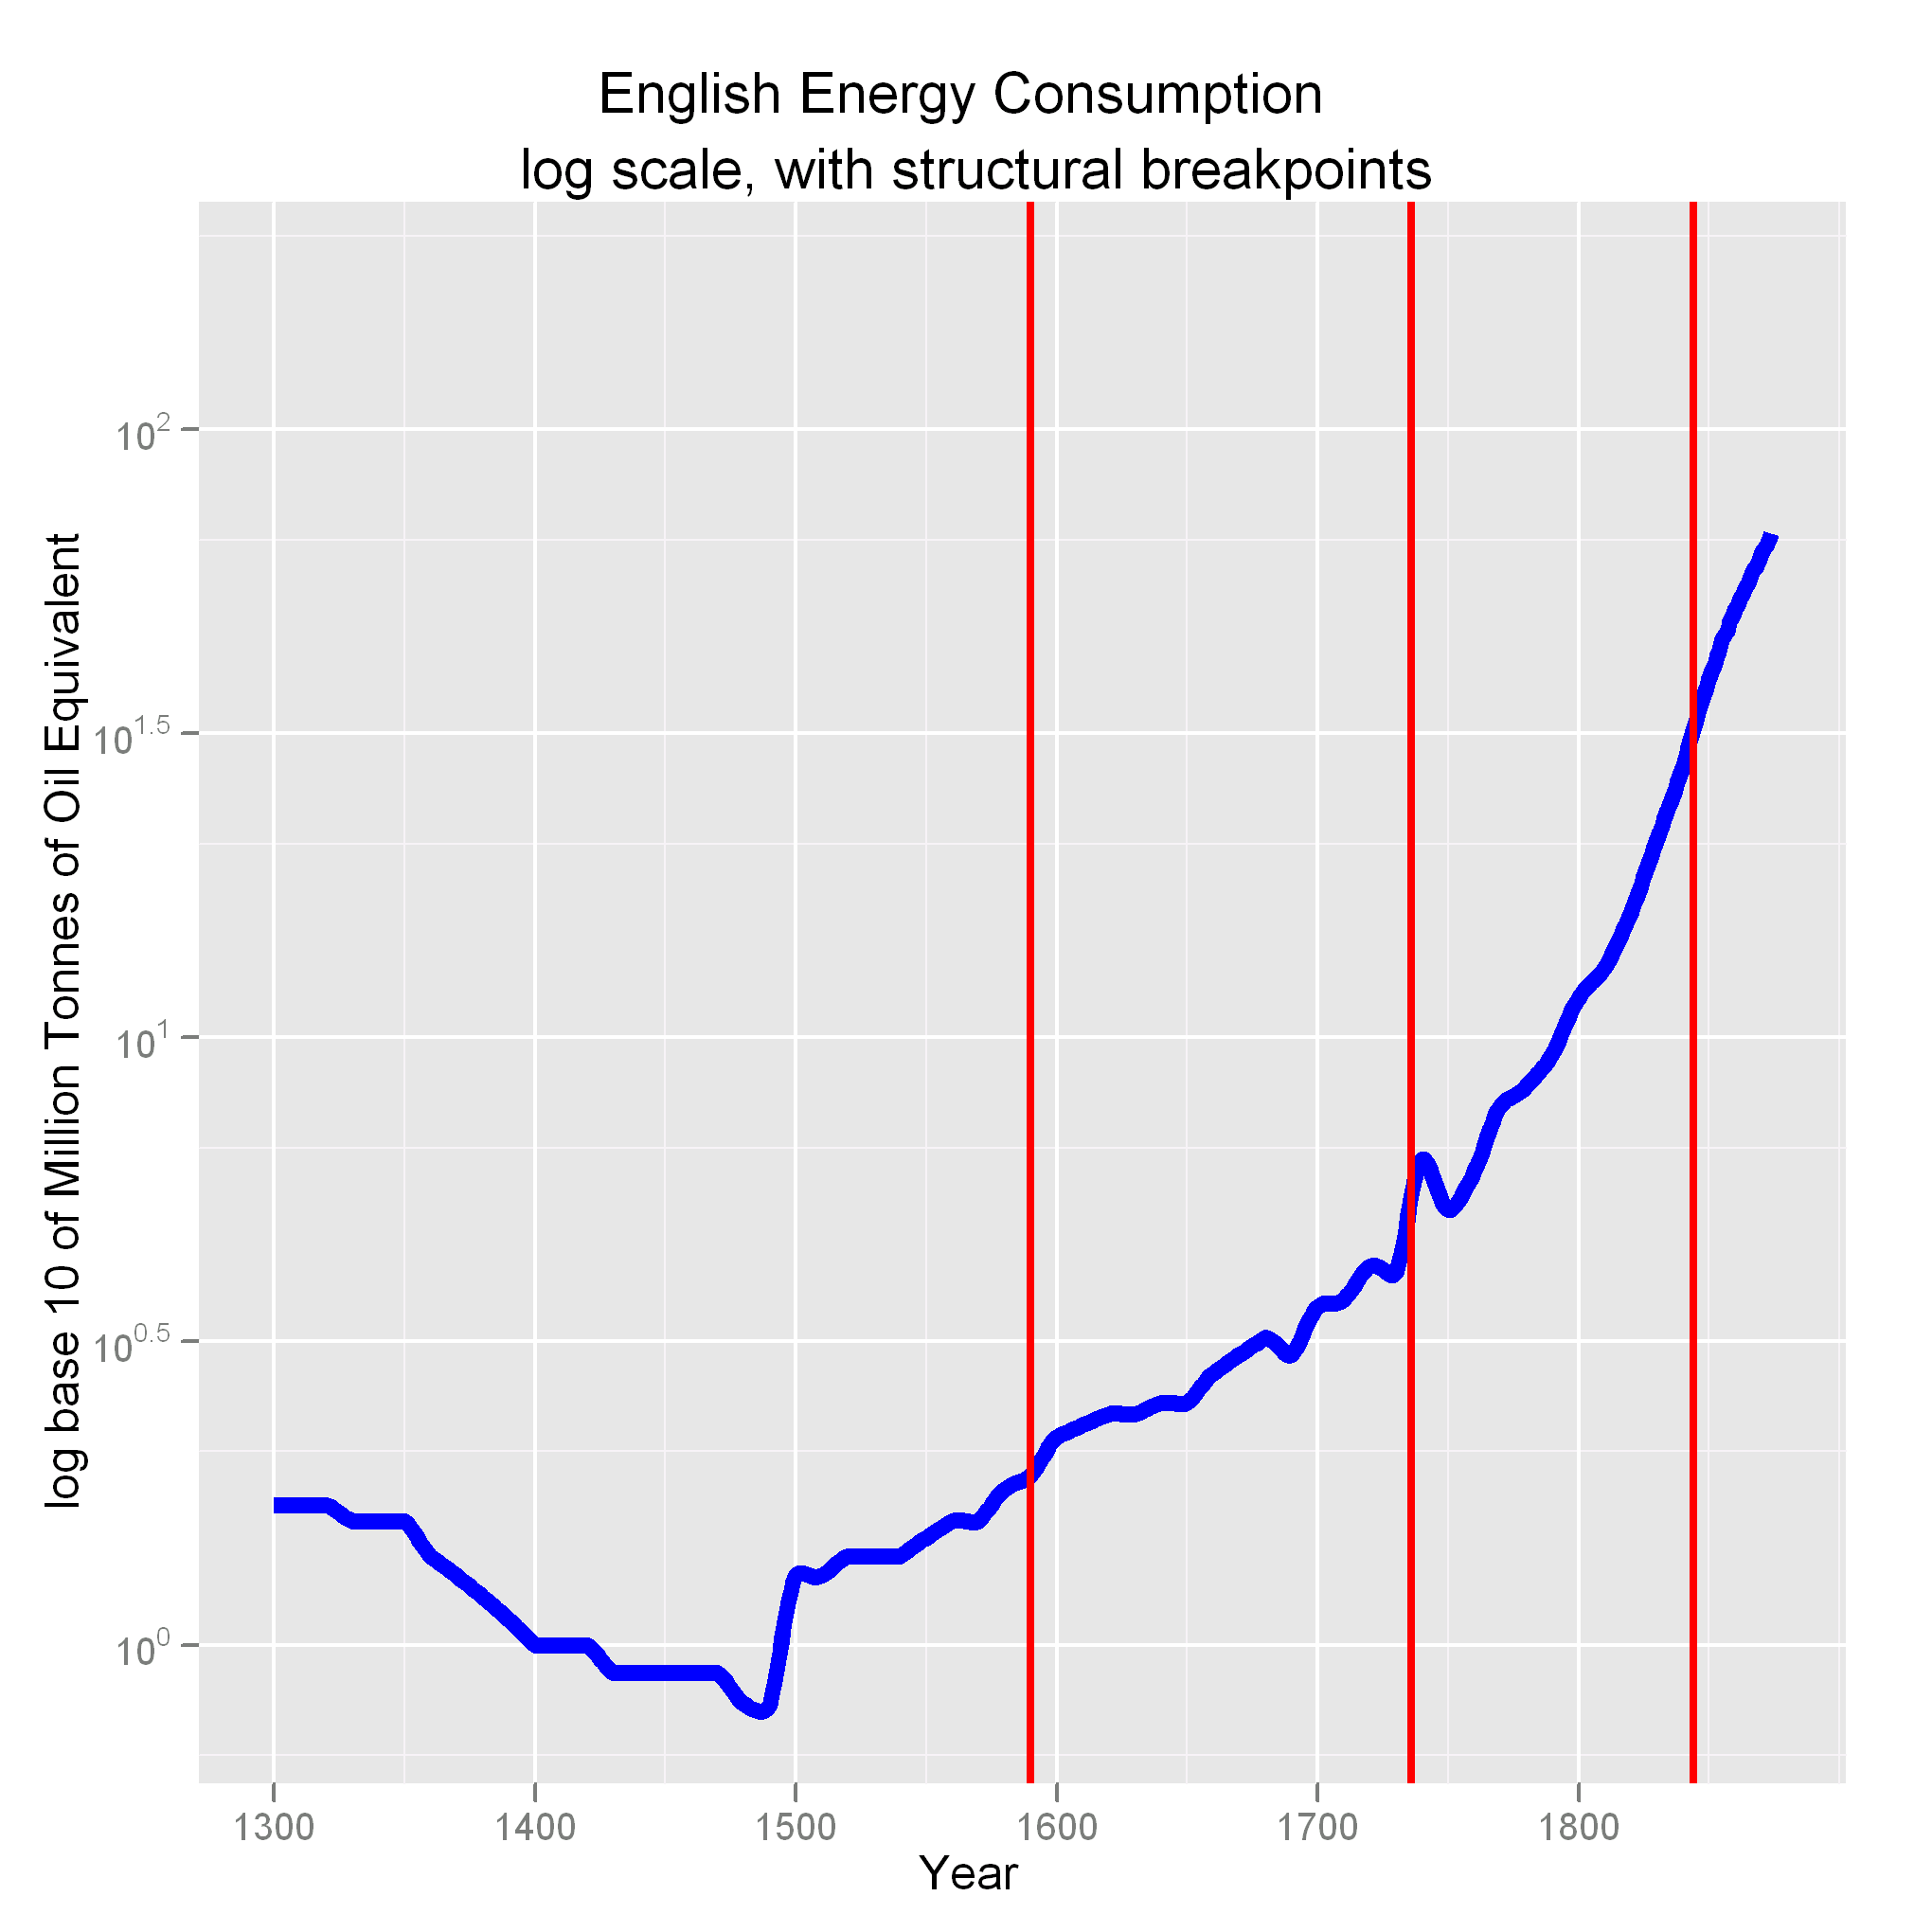
\includegraphics[width=0.33\textwidth]{../data/Analytics/notes/gbpmtoelog.png}
		\label{fig:subfig2}}
		\subfloat[diff \textit{log} energy consumption][Difference of \textit{log} of English energy consumption]{
		\includegraphics[width=0.33\textwidth]		{../data/Analytics/notes/gdifflogmtoe.png}
		\label{fig:subfig3}}
		
		\end{figure}
		

		\begin{figure}
%		\centering

		\caption[Levels, \textit{log} of levels and diffs of the time series]{Levels, \textit{log} of levels and first differences of logs of English GDP, with statistically significant breakpoints indicated by vertical lines on the log chart.}			\label{fig:globfig2}
				
		\subfloat[\textit{level} GDP][English GDP in levels]{
		\includegraphics[width=0.33\textwidth]{../data/Analytics/notes/ggdp.png}
		\label{fig:subfig4}}
		\subfloat[\textit{log} GDP][\textit{log} of English GDP]{
		\includegraphics[width=0.33\textwidth]{../data/Analytics/notes/gbpgdplog.png}
		\label{fig:subfig5}}
		\subfloat[diff \textit{log} energy consumption][Difference of \textit{log} of 				English energy consumption]{
		\includegraphics[width=0.33\textwidth] 	{../data/Analytics/notes/gdiffloggdp.png}
		\label{fig:subfig6}}
		
		\end{figure}

		\begin{figure}
		\centering

		\caption[Levels, \textit{log} of levels and diffs of the time series]{Levels, \textit{log} of levels and first differences of logs of the English population, with statistically significant breakpoints indicated by vertical lines on the log chart.}						\label{fig:globfig3}
		
		\subfloat[\textit{ln} population][\textit{ln} of English population in levels]{
		\includegraphics[width=0.33\textwidth]{../data/Analytics/notes/gpop.png}
		\label{fig:subfig7}}
		\subfloat[\textit{log} GDP][\textit{log} of English GDP]{
		\includegraphics[width=0.33\textwidth]{../data/Analytics/notes/gbppoplog.png}
		\label{fig:subfig8}}
		\subfloat[\textit{ln} diff population][\textit{ln} of first differences of English population]{
		\includegraphics[width=0.33\textwidth]{../data/Analytics/notes/gdifflogpop.png}
		\label{fig:subfig9}}
		
		\end{figure}		
		
%		\includepdfmerge[nup=2x3,noautoscale=true,scale=0.4,frame=true,offset=0 				-50,delta=0 10]						{../data/Analytics/notes/bpmtoe.png,../data/Analytics/notes/diffmtoe.png, ../data/Analytics/notes/bpgdp.png,../data/Analytics/notes/diffgdp.png, ../data/Analytics/notes/bppop.png,../data/Analytics/notes/diffpop.png}

%	\caption[
%	\textit{Ln} of levels and diffs of the time series]{\textit{Ln} of levels and first differences of the English time series, with statistically significant breakpoints indicated by vertical lines on the levels charts}


\newpage		
		\subsubsection{Stationarity}
		
		To further characterize the time-series, I tested each as a univariate \gls{arima} model using the $R$ \texttt{forecast} package \cite{hyndman_forecast:_2010}. The \texttt{auto.arima} method in \texttt{package::forecast} selects the appropriate model and allows incorporating exogenous (non-stochastic) inputs such as the time-series intervention variables described above.
		
		I note that after allowing for event interventions, both MTOE and GDP are $I(1)$ (non-stationary, or integrated of order one, mean a first difference or first derivative will be stationary. The population series is modeled as $I(0)$ (stationary), though the event interventions are not significant in this analysis. Each series analyzed without event dummies indicates $I(2)$, confirming the visual inspection results from figure \ref{fig:globfig1}.

		

		\begin{table}[h!]

		\begin{adjustwidth}{-0.75in}{}

		\caption[Summary \texttt{auto.arima} results]{This table contains the 		summary of the \texttt{auto.arima} analyses showing the results for no time intervention variables, and for results with time intervention variables}\label{tbl:station}

		\begin{tabular}{llrrrrrrrrr}
		\toprule \hline
		Breaks&Model&&Model&Variables&&&&&&\\
		\toprule \hline
		&MTOE&ar1&ar2&ar3&ar4&ma1&S1&S2&S3&drift\\
		\hline
		None&ARIMA(4,2,1)&0.8385& 0.5742&  -0.2776&  -0.3054&  -0.9334&&&\\
	    &s.e.        &0.0457&  0.0531&   0.0541&   0.0431&   0.0306&&&\\
		\hline
1590&ARIMA(4,1,1)&0.1880&1.3171&0.0014&-0.6435&0.8857&0.0065&0.0001&0.0004&-0.0049\\
1736&with drift&0.0354&0.0374&0.0341&0.0325&0.0270&0.0016&0.0016&0.0016&0.0019\\
1844&&&&&&&&&&\\
		\midrule \hline
		&GDP&ar1&ar2&ma1&ma2&ma3&ma4&S1&S2&S3\\
		\toprule
		None&ARIMA(1,2,4)&-0.6596&&0.3130&-0.6897&-0.1270&-0.1022&&&\\
	    &s.e.        &0.0608 &&0.0684&0.0492 &0.0613 &0.0531&&&\\
		\midrule
1556&ARIMA(2,1,3)&0.2427&0.7438&0.4158&-0.7589&-0.1777&&-0.0067&0.0030&-0.0156\\
1731&s.e.        &0.0467&0.0466&0.0634&0.0358&0.0600&&0.0030&0.0025&0.0062\\
1869&&&&&&&&&&\\
		\midrule \hline
		&Population&ar1&ar2&ma1&ma2&ma3&intercept&S1&S2&S3\\
		\toprule
		None&ARIMA(0,2,3)&&&-0.2994&-0.2525&-0.1521&&&&\\
	    &s.e.        &&&0.0410&0.0426&0.0411&&&&\\
		\midrule
1373&ARIMA(2,0,3)&1.9912&-0.9912&-0.2956&-0.2498&-0.1502&15.3036&-0.0016&-0.0017&-0.0017\\
1579&s.e.        &0.0072& 0.0072& 0.0416& 0.0429& 0.0415&    NaN& 0.0033&0.0033&0.0033\\
1774&&&&&&&&&&\\
		\bottomrule

		\end{tabular}
		\end{adjustwidth}
		\end{table}
		
		\newpage
		\subsubsection{Cointegration}
		
		Finally in this preliminary analytic exercise, I investigate the cointegration properties of the information set. To do so, I use the $R$ package \texttt{urca} as implemented from work done by Bernard Pfaff \cite{pfaff_analysis_2008}.
		
		The results are summarized in Table \ref{tbl:coint}. I model each series as a bivariate pair to assess the strength of any indicated cointegration relations and to support the multivariate modeling for the main analysis. I also model with different lag structures to assess robustness. The most robust bivariate result is between the MTOE and GDP pairs, with the second between the GDP and population pairs. These results support the multivariate modeling which indicates two cointegrating relations.
		
		The noteworthy result is that the cointegration relation between energy consumption and GDP is very strong, supporting my research hypothesis. These are preliminary, but encouraging, results. Further statistical testing awaits approval of this proposal.
		
		I also need to switch to the most robust cointegration software available, which is CATS in RATS as my analysis proceeds.
		

		\begin{table}[h!]
		\begin{center}
\caption[Johansen cointegration tests]{Johansen cointegration tests for English energy demand system; sample period 1300 - 1874 CE}\label{tbl:coint}
	
\begin{tabular} {llllrll}
\toprule \hline
&&No.&&&&\\
&Deterministic&of lagged&&Test& \multicolumn{2} {c} {Critical values} \\
\cmidrule (lr) {6-7}
Variables&terms&differences&$H_0:r=r_0$&statistic&$10\%$&$5\%$\\
\midrule
$e,g$&$tr,shift$&1&$r_0=0$&45.18&22.76&25.32\\
&&&$r_0=1$&0.81&10.49&12.25\\
&&&&&&\\
&&2&$r_0=0$&33.21&22.76&25.32\\
&&&$r_0=1$&0.79&10.49&12.25\\
&&&&&&\\
$e,p$&$tr,shift$&1&$r_0=0$&41.49&22.76&25.32\\
&&&$r_0=1$&12.45&10.49&12.25\\
&&&&&&\\
&&2&$r_0=0$&33.51&22.76&25.32\\
&&&$r_0=1$&10.20&10.49&12.25\\
&&&&&&\\
$g,p$&$tr,shift$&1&$r_0=0$&43.29&22.76&25.32\\
&&&$r_0=1$&6.02&10.49&12.25\\
&&&&&&\\
&&2&$r_0=0$&35.73&22.76&25.32\\
&&&$r_0=1$&5.97&10.49&12.25\\
&&&&&&\\
$e,g,p$&$tr,shift$&1&$r_0=0$&78.54&39.06&42.44\\
&&&$r_0=1$&41.45&22.76&25.32\\
&&&$r_0=2$&5.16&10.49&12.25\\
&&&&&&\\
&&2&$r_0=0$&63.06&39.06&42.44\\
&&&$r_0=1$&28.94&22.76&25.32\\
&&&$r_0=2$&5.42&10.49&12.25\\
\bottomrule
\end{tabular}

\caption*{\textit{Notes:} \textit{e}-ln of MTOE (million tonnes of oil equivalent), \textit{g}-ln of GDP, \textit{p}-ln of population. For the model's deterministic components: \textit{c}-constant, \textit{tr}-linear trend, \textit{shift}-shift dummy $dsubS3$; critical values from Johansen.}
\end{center}
\end{table}

		\newpage


	\section{Completion Timetable}
		\begin{tabular}{ll}
		Event&Date\\
		\midrule
		Draft Proposal&August 2011\\
		Topic Defence&Spring 2012\\
		Draft Dissertation&Fall 2012\\
		Final Defence&Fall 2012\\
		\bottomrule
		\end{tabular}
	
	
	\section{Annotated Bibliography}
		\bibliography{scbdissertation}
%		\bibliography{exporteditems}
	
	\section{Glossary}
	\printglossaries
	
\begin{comment}
$12^{th}$ century renaissance \url{http://en.wikipedia.org/wiki/Renaissance_of_the_12th_century}
\end{comment}

\appendix
\section{Detailed Statistical Methodology} 
\label{sec:Appendix A}

	Note that these step-by-step details are mainly notes to myself regarding the Copenhagen methodology at a detailed level. I include them here for interested readers, but the proposal should be understandable without this detail for most.

			\begin{enumerate}

				\item Description of the logic of the methodology (the probability approach in VAR econometrics):
				
				 ``The vector autoregressive (VAR) process based on Gaussian (normally distributed) errors has frequently been a popular choice as a description of macroeconomic time-series data.
				
			Theory-based economic models have traditionally been developed as non-stochastic mathematical entities and often applied to empirical data by adding a stochastic error process to the mathematical model.
			
			From an econometric point of view, the two approaches are fundamentally different: one starting  from an explicit stochastic formulation of \textit{all} data and then \textit{reducing} the general statistical (dynamic) model by imposing testable restrictions on the parameters, the other starting from a mathematical (static) formulation of a theoretical model and then \textit{expanding} the model by adding stochastic components.''
			\footnote{Juselius 2006 chapters 1--3} %%Juselius 2006 ch1-3

				\item Investigate the unrestricted VAR
				\begin{enumerate}
					\item Estimate the unrestricted VAR for the information set
					\item Select and form the \gls{ecm} representation
					\item Perform misspecification tests
					\begin{enumerate}
						\item Perform specification checking
						\item Test residual correlations and use information criteria to identify lag lengths
						\item Test residual autocorrelation 
						\item Test residual heteroskedasticity
						\item Perform normality tests
					\end{enumerate}
				\end{enumerate}
				\item Investigate deterministic components in the model. \footnote{Juselius 2006 chapter 6} %% Juselius ch6
				\begin{enumerate}
					\item Identify possible deterministic cases. The reference model is the simple $VAR(1)$ containing a constant, $\boldsymbol{\mu}_0$, and a trend, $\boldsymbol{\mu}_1t$ in $AR$ form:
					\begin{equation}
					\Delta \bold{x}_t = \boldsymbol{\alpha \beta}'\bold{x}_{t-1} + \boldsymbol{\mu}_0 + \boldsymbol{\mu}_1t + \boldsymbol{\epsilon}
					\end{equation}
					\begin{enumerate}
						\item Case 1. $\boldsymbol{\mu}_1$, $\boldsymbol{\mu}_0 = \bold{0}$. This case corresponds to a model with no deterministic components in the data, i.e. $E(\bold{\Delta} \bold{x}_t)=\bold{0}$ and $E(\boldsymbol{\beta}^{'} \bold{x}_t) = \bold{0}$
						\item Case 2. $\boldsymbol{\mu}_1=\bold{0}$, $\boldsymbol{\gamma}_0=\bold{0}$ but $\boldsymbol{\beta}_0 \neq \bold{0}$, where $\boldsymbol{\gamma}_0$ is defined as a term in the decomposition of $\boldsymbol{\mu}_0=\boldsymbol{\alpha \beta}_0 + \boldsymbol{\gamma}_0$.
						\item Case 3. $\boldsymbol{\mu}_1= \bold{0}$, i.e. $(\boldsymbol{\beta}_1, \boldsymbol{\gamma}_1)= \bold{0}$, and the constant term $\boldsymbol{\mu}_0$ is \textit{unrestricted}, i.e. no linear trends in the $VAR$ model, but linear trends in the variables, where $\boldsymbol{\gamma}_1$ is defined as a term in the decomposition of $\boldsymbol{\mu}_1=\boldsymbol{\alpha \beta}_1 + \boldsymbol{\gamma}_1$.
						\item Case 4. $\boldsymbol{\gamma}_1 = \bold{0}$, but $(\boldsymbol{\gamma}_0,\boldsymbol{\beta}_0,\boldsymbol{\beta}_1) \neq \bold{0}$, i.e. the trend is \textit{restricted} only to appear in the conintegrating relations, but the constant is unrestricted in the model.
						\item Case 5. No restrictions on $\boldsymbol{\mu}_0, \boldsymbol{\mu}_1$, i.e. trend and constant are \textit{unrestricted} in the model.
					\end{enumerate}
					\item In $MA$ common trends form to clarify the source of linear trends:
					\begin{equation}
					\bold{x}_t = \boldsymbol{\beta}_\bot(\boldsymbol{\alpha}_\bot ' \boldsymbol{\Gamma} \boldsymbol{\beta}_\bot)^{-1} \boldsymbol{\alpha}_\bot '\left\lbrace \boldsymbol{\gamma}_0 t + \frac{1}{2} \boldsymbol{\gamma}_1 t + \frac{1}{2} \boldsymbol{\gamma}_1 t^2 \right\rbrace + \bold{C}^*(L) \boldsymbol{\mu}_1 t
					 + \bold{C}^*(1) \boldsymbol{\mu}_0 + \bold(C) \displaystyle\sum\limits_{i=1}^t \boldsymbol{\epsilon}_t + \bold{C}^*(L) \boldsymbol{\epsilon}_t + \bold{\tilde{X}}_0
					\end{equation}
					Thus, the linear trends in the variables can originate from three different sources in the $VAR$ model:
					\begin{enumerate}
						\item[1.] the $\boldsymbol{\alpha}$ component $(\bold{C}^*(L) \boldsymbol{\mu}_1 t)$ of the unrestricted linear trend $\boldsymbol{\mu}_1 t$;
						\item[2.] the $\boldsymbol{\beta}_\bot$ component $(\boldsymbol{\gamma}_1 t)$ of the unrestricted linear trend $\boldsymbol{\mu}_1 t$;
						\item[3.] the $\boldsymbol{\beta}_\bot$ component $(\boldsymbol{\gamma}_0 t)$ of the unrestricted constant term $\boldsymbol{\mu}_0$.
					\end{enumerate}
					\item Consider intervention \textit{(dummy)} variables. Similarly as for the trend and constant, consider a simple regression model for $x_t$ containing three different types of dummy variables:
					\begin{equation}
					x_t = \phi_s D_{s,t} + \phi_p D_{p,t} + \phi_{tr} D_{tr,t} + u_t + x_0
					\end{equation}
					where $D_{s,t}$ is a mean-shift dummy $(\dots,0,0,0,1,1,1,\dots)$, $D_{p,t}$ is a permanent intervention dummy $(\dots,0,0,1,0,0,\dots)$, and $D_{tr,t}$ is a transitory shock dummy $(\dots,0,0,1,-1,0,0.\dots)$ and the residual is a first order autoregressive process with form:
					\begin{equation}
					u_t = \frac{\epsilon_t}{1-\rho L}
					\end{equation}
					Which for difference non-stationary series results in a change of form as follows:
					\begin{equation}
					\Delta x_t = \phi_s \Delta D_{p,t} + \phi_p \Delta_{tr,t} + \phi_{tr} \Delta_{dtr,t} +  \epsilon_t,
					\end{equation}
					i.e. a shift in the levels of a variable becomes a `blip' in the difference variable, a permanent `blip' in the levels becomes a transitory blip in the differences, and a transitory blip in the levels becomes a double transitory blip, $D_{dtr,t}$, in the differences.
					
					My plan is to analyse the time series for structural breaks, formulate dummy variable(s) appropriately, then test whether the dummies are significant, and for which equations in the $VAR$.
				\end{enumerate}
				\item Estimate the $I(1)$ model. \footnote{Juselius 2006 chapter 7} %%Juselius ch7
				\begin{enumerate}
					\item Preliminary estimates of the English data indicate that the series, \textit{with time dummies included}, are integrated of order one $I(1)$.  This, of course, is essential in determining the formally correct methodology as $I(2)$ forms require a modified technique.  However, practical considerations, for example lack of $I(2)$ support in current software, dictate that I will use $I(1)$ methodology, BUT will check for signalling of $I(2)$ problems.
					\item Concentrating the general $VAR$ model.
					
					Proceeding under the $I(1)$ assumption, and under the assumption that the empirical $VAR$ can describe the data, we can state the $I(1)$ condition as:
					\begin{equation}
					\boldsymbol{\Pi} = \boldsymbol{\alpha \beta'},
					\end{equation}
					where $\boldsymbol{\alpha}$ and $\boldsymbol{\beta}$ are $p \times r$ matrices.  If $r = p$, then $\bold{x}_t$ is stationary and classical inference applies.  If $r = 0$, then there are $p$ autonomous trends in $\bold{x}_t$ so that each $x_{i,t}$ is non-stationary with its own individual trend.  In this case the vector process is driven by $p$ different stochastic trends and it is not possible to obtain stationary cointegration relations between the levels of the variables.  Also, the variables have no stochastic trends in common and, hence, do not move together over time.
					
					Should this be the case, I will reformulate the $VAR$ model in levels as a $VAR$ model in differences \textit{without any consequential loss of long-run information} and classical inference applies.
					
					If $p > r > 0$, then $\bold{x}_t \sim I(1)$ and there exist $r$ directions into which the process can be made stationary by linear combinations.  These are the cointegrating relations, which often can be interpreted as deviations from economic steady-state relations, and are thus economically meaningful.
					\item Derive the maximum likelihood (ML) estimator of the concentrated model.
					
					Assuming a finding of cointegrating relations, I proceed to use ML to estimate the long-run equilibrium relations from a concentrated model of the form (disregarding for the moment deterministic elements):
					\begin{equation}
						\bold{R}_{0t} = \boldsymbol{\alpha \beta'}\bold{R}_{1t} + \boldsymbol{\epsilon}_t, \quad \boldsymbol{\epsilon}_t \sim N_p(\bold{0},\boldsymbol{\Omega}).
					\end{equation} Note that at this point the estimating task has been separated into long-run and short-run processes, an essential part of the methodology, and allowed under the Frisch-Waugh theorem.
					\item Normalize the results.
					
					This step allows an economic interpretation of a cointegrating relation, and thus one should choose a meaningful normalizing variable. Note, however, that the cointegrating relations are not sensitive to the choice of normalizing variable. Note that this is the so-called ``Johansen" procedure.
					\item Interpret the unrestricted results.
					
					While the unrestricted $\boldsymbol{\hat{\alpha}, \,\hat{\beta}, \text{ and } \hat{\Pi}}$ are not expected to yield directly interpretable results, they may, so I will proceed by inspecting them.
				\end{enumerate}
				\item Determine the cointegration rank. \footnote{Juselius 2006 chapter 8}  %%Juselius ch 8
				
				This is an essential step as it influences subsequent inference and economic interpretation. The actual test statistics are likelihood ratios (LR), and are compared to carefully specified asymptotic distributions to yield critical values.
				
				The cointegrating rank divides the data into $r$ relations towards which the process is adjusting, and $p - r$ relations which are pushing the process. The former are interpreted as (initially) statistical equilibrium errors (deviations from a statistical steady-state), and the latter as common driving trends in the system.
				\item Cointegration hypotheses testing--recursive tests of parameter constancy. \footnote{Juselius 2006 chapter 9}
				
				In this step I will perform four classes of tests for parameter constancy, using both statistical and graphical methods.
				\begin{enumerate}
					\item Recursive tests of the full model, essentially a recursive test of the likelihood function, which will indicate whether the model is approximately acceptable.  This is conceptually similar to recursive Chow tests for single-equation models.
					\item Recursive tests on the eigenvalues, $\lambda_i$ and transformations of them, which will provide more detailed constancy information about individual cointegrating relations.
					\item Recursive tests of the constancy of the cointegration space, $\boldsymbol{\beta' x_t}$.
					\item Recursive tests of predictive failure for both the full system and individual series.
					\item Judging the effects of any found parameter instability.
				\end{enumerate}
				\item Cointegration hypotheses testing--testing restrictions on $\boldsymbol{\beta}$. \footnote{Juselius 2006 chapter 10}
				
				This process will help in spotting potentially relevant long-run relations, and requires several steps:
				\begin{enumerate}
					\item Formulate hypotheses as restrictions on $\boldsymbol{\beta}$.
					\item Testing the same restriction on all cointegration relations.
					\item Testing the stationarity of a known $\boldsymbol{\beta}$ vector.
					\item Testing the stationarity of a cointegration relation when some coefficients are know and others must be estimated.
				\end{enumerate}
				\item Cointegration hypotheses testing--testing restrictions on $\boldsymbol{\alpha}$. \footnote{Juselius 2006 chapter 11}
				
				Tests on $\boldsymbol{\alpha}$ are closely associated with interesting hypotheses about the common driving forces in the system.  
				
				The test of zero row in $\boldsymbol{\alpha}$ is the equivalent of testing whether a variable can be considered weakly exogenous for the long-run parameters $\boldsymbol{\beta}$.  These define a common driving trend as cumulative sums of empirical shocks to variables.
				
				The test of a unit vector in $\boldsymbol{\alpha}$ defines a variable which is exclusively adjusting, and whose shocks have no permanent effect on any of the variables in the system.
				
				Thus, the two types of test can identify the pushing and pulling forces of the system.
				\begin{enumerate}
					\item Testing for long-run weak exogeneity.
					\item Testing for weak exogeneity in partial models.
					\item Testing a known vector in $\boldsymbol{\alpha}$.
					\item Interpret the results on $\boldsymbol{\beta}$ and $\boldsymbol{\alpha}$ in terms of economic scenarios.
				\end{enumerate}
				\item Identification--identify the long-run structure. \footnote{Juselius 2006 chapter 12} %%Juselius 2006  ch 12
				\begin{enumerate}
					\item Formulate identifying hypotheses and degrees of freedom
					\item Consider just-identifying restrictions
					\item Consider over-identifying restrictions
					\item Consider lack of identification
					\item Perform recursive diagnostic tests of $\alpha$ and $\beta$
				\end{enumerate}
				\item Identification--identify the short-run structure. \footnote{Juselius 2006 chapter 13}	%% Juselius 2006 ch 13
				\begin{enumerate}
					\item Formulate identifying restrictions
					\item Interpret shocks
					\item Formulate the short-run economic questions
					\item Consider restrictions on the short-run reduced-form model
					\item Construct \textit{VAR} in triangular form
					\item Formulate empirically identifiable current effects
					\item Construct the preferred structure
				\end{enumerate}
				\item Identification--identify common trends. \footnote{Juselius 2006 chapter 14} %%Juselius 2006 ch 14
				\begin{enumerate}
					\item Formulate the common trends representation
					\item Formulate the unrestricted MA representation
					\item Formulate the MA representation subject to restrictions on $\alpha$ and $\beta$
					\item Impose exclusion restrictions on $\beta_\bot$
					\item Assess the economic model scenario
				\end{enumerate}
				\item Identification--identify a structural MA model. \footnote{Juselius 2006 chapter 15} %% Juselius ch 15
				\begin{enumerate}
					\item Reparameterize the VAR model
					\item Separate between transitory and permanent shocks
					\item Formulate and interpret structural shocks
					\item Test the credibility of the labels on the economic shocks
				\end{enumerate}
			\end{enumerate}
			
\section{Table of variable, coefficient, and function definitions} 
\label{sec:Appendix B}
\centering
%\begin{center}
\begin{longtable}{ll}
\toprule
Variable&Description\\
\toprule
$\bold{x}_i , i=0 \cdots k-1$&m x 1 vector of endogenous variables\\
$m$&number of endogenous variables\\
$k$&number of lags for independent endogenous variables\\
$\Delta \bold{x}_i$&first difference of endogenous variables\\
$\boldsymbol{\mu}_0$&m x 1 vector of intercept coefficients\\
$\boldsymbol{\mu}_1$&m x 1 vector of time-dependent coefficients\\
$t$&sequentially enumerated time period\\
$AR$&auto-regressive specification\\
$E$&probabilistic expectations operator\\
$\boldsymbol{\Pi}(=\boldsymbol{\alpha}\boldsymbol{\beta}')$&m x m matrix of dynamic coefficients relating $\Delta \bold{x}_t$ to past values of $\bold{x}_t$\\
$\boldsymbol{\alpha}$&m x r matrix of adjustment coefficients describing how equilibrium deviations feed back onto $\bold{x}_t$\\
$\boldsymbol{\beta}'$&r x m matrix of deviations from equilibrium\\
$r$&number of cointegrating relationships\\
$\boldsymbol{\gamma}$&a term which allows us to decompose $\boldsymbol{\alpha\beta}'$ into further usable terms\\
$MA$&moving average common trends specification\\
$\boldsymbol{\beta}_\bot$&orthogonal complement of $\boldsymbol{\beta}'$\\
$\boldsymbol{\alpha}'_\bot$&orthogonal complement of $\boldsymbol{\alpha}$\\
$\boldsymbol{\Gamma}$&m x m matrix of coefficients relating $\Delta \bold{x}_t$ to past values of $\Delta \bold{x}_{t-i}$\\
$\bold{C}$&m x m matrix of coefficients in moving average representation of VAR to evaluate deterministic trends in cointegrating relationships\\
$L$&lag operator representing the number of past periods of endogenous variable data to be included\\
$\bold{R}$&concentrated notation of VAR model for notational simplicity\\


\end{longtable}
%\end{center}

\end{comment}

\end{document}

\section{End}

\section{notes}

\subsection{committee notes}
Tim -- remove personal references e.g. Marx  %done 10/13/11
Tim -- quantitative measure of unlimited energy % so lewis talked about labour with at zero marginal product. my idea is that, relative to any labor supply, the amount of mineral energy was essentially unlimited for the initial developing economies. another way of thinking of it is the human energy chart. an interesting question is whether pure energy has diminish marginal product, I think not, thus that you have to look at specific sources and their physical requirements to determine the amount of diminishing marginal product, and in any case it is less than human labour.  10/13/11. %done 11/14/11.

Richard -- other metric approaches. %Why, since looking at graphs of gdp and energy consumption per capita presents such a clear relationship, do I consider a more detailed statistical look? I am interested in looking inside the dynamics that are supported by the long period time series. What this examination should tell is whether the the prime dynamic drivers, so the leading-in-time variables, changed places in the short run and the long run in the economies I study. While I purposefully avoid the term causality at this point, depending on the strength of the results, I may find causality in the data. What I want to understand, beyond my hypothesis of centrality of mineral energy consumption as the defining invention of the Industrial Revolution, is what implications this has for modern development and for sustained per capita economic development in an age of potentially emission constrained economies. The time series methodology I propose has the ability to do this. And it has the capability of incorporating important time related events that enter the time series as discontinuties. Both of these capabilities are core to my research. 10/14/11. %done 11/14/11.

11/17
Rudi - 5 major items. mainly tighten. He thinks if I do a 2-3 page abstract of intro section, Lance might be interested.

You've done already a lot of work. On a lot of this I am no expert (neither history nor metrics). So bear with me.
Let me jot down just a few quick notes:


\begin{itemize}
\item 1) Presentation: Put hypothesis first; don't make the reader wait or search. In this draft, and in a later paper, and in your presentation, the juxtaposition of the various explanations should come much earlier. I.e.: On the first page (!!), there should be a paragraph saying that "the industrial revolution in England is commonly explained by (1) cultural exceptionalism, wihch essentially means ... , (2) ... , (3) energy, .... (4) thermodynamics. My hypothesis is that (x) matters more than previously believed, and my dissertation tests the evidence for that. The anecdotal evidence includes the lack of Dutch industrialization ... etc. " 

\item 2) Hypothesis: Sharpen it. How distinct is your hypothesis really from culture/institution-driven explanations? You do argue that all, even cultural exceptionalists, place emphasis on coal. It might be reasonable to say that the explanation must be found in a combination of these factors -- and your contribution is to "shift the weights." Is that about right? It could be fleshed out more, sharpened at the edges.

\item 3) Metrics: Institutional variables. I didn't go through the details. Do you use some proxies for institutional development, or cultural factors? Should that be there, if you want to compare the influence of those variables to energy? 

\item 4) Contributions: Limit yourself. Section 2.1.2 is too broad, and contains too much, I would say. It is not clear what you mean by 5., and, if clarified, it is by itself possibly a whole dissertation. I would drop it for now. 3. and 4. should go together. Arguably, 4. might be post-dissertation research. You want a classic 3 goals (and papers) in here: (1) Literature review, which you've done in part;  (2) Explanation and re-evaluation of the industrial revolution in England in the language of economic history; (3) Explanation and re-evaluation of the industrial revolution in England in the language of econometrics. 

\item 5) The link to growth theory: Rather than 5., you might want to consider "old" growth theories. You make reference to Lewis. So combine Lewis (or Marx and Kalecki, really) with Malthus, and see where that takes you. Lewis warns of the turning point, when surplus labor is exhausted, and real wages must rise. If energy is the real labor, then we might be there. What does that mean for future growth? That's an interesting question, and you can fruitfully feed future research --- but I would try to make these three papers quite focused on what you have in mind now. 

\end{itemize}


thinks I could do england vs holland and nail that. would need dutch energy series.

Tim - wants me to change graphs, support his method, has many notes, likes my lit review.

\begin{itemize}
\item 
\end{itemize}

\begin{itemize}
\item Why time series
\item Various ts approaches
\item univariate arima
\item static
\item ardl
\item var
\item cointegrated var

\end{itemize}

may use the Diebold 98 article for organizing, or Dougherty

\subsection{sequence for bibliography}

pdflatex
bibtex on .bib F11
pdflatex
pdflatex
bibtex on .tex  F11
pdflatex
pdflatex

sequence for glossary

    Build LaTeX document, this will generate the files used by makeglossaries
    Run the indexing/sorting, the recommended way is to use makeglossaries (a script that runs xindy or makeindex depending on options in the document with correct encoding and language settings):

    makeglossaries <myDocument>

    Build LaTeX document again to get document with glossary entries


\begin{comment}
% save just for reference...covered by table and annotated bib
		\subsection{Data Sources}
		I anticipate using a wide variety of sources. Should I just do a bibliography here?
			\subsubsection{English historical-institutional sources}
			\begin{itemize}
			\item Wrigley
			\item van Zanden
			\item for reference, list in Wrigley discussion
			\item Landes
			\item Crafts
			\item Temin
			\item Pomeranz
			\item Allen
			\item Mokyr
			\item Goldstone
			\item McCloskey
			\item de Vries
			\item Jevons
			\item Clark
			\item TS Ashton
			\end{itemize}
			\subsubsection{English long-period time series sources}
			\begin{itemize}
			\item Mitchell
			\item Snooks
			\item Officer
			\item Fouquet
			\item Warde
			\item Maddison
			\end{itemize}
			\subsubsection{U.S. historical-institutional sources}
			\begin{itemize}
			\item Vaclav Smil
			\item Daly and Townsend
			\item Lewis
			\item North
			\end{itemize}
			\subsubsection{U.S. long-period time series sources}
			\begin{itemize}
			\item Historical Statistics of the United States 1780-1945
			\item Historical Statistics of the United States Millennial Edition Online
			\item Historical, Demographic, Economic, and Social Data: The United States, 1790-2002
			\item Gordon Whitney
			\item Kindleberger
			\end{itemize}
			\subsubsection{Chinese historical-institutional sources}
			\begin{itemize}
			\item Xu, Dixin, and Zhengming Wu, eds. 2000. Chinese Capitalism, 1522-1840. New York: St. Martin's Press.
			\item Hsien-Chun Wang. 2009. ``Discovering Steam Power in China, 1840s-1860s." Technology and Culture 51(1): 31-54.
			\item ``Pomeranz, K.: The Great Divergence: China, Europe, and the Making of the Modern World Economy."
			\item Andre Gunder Frank
			\item Janet Abu-Lughod
			\item Jack Goldstone
			\end{itemize}
			\subsubsection{Chinese long-period time series sources}(May not be available)
			\begin{itemize}
			\item Sinton, Jonathan E. 2001. ``Accuracy and reliability of China's energy statistics." China Economic Review 12(4): 373-383.
			\item Chinese Statistical Yearbook
			\end{itemize}
			\subsubsection{World long-period time series sources}
			\begin{itemize}
			\item Payne - a literature review of recent energy-gdp empirical studies
			\item US DOE EIA
			\item OECD
			\item UN
			\item Katarina Juselius. 2010. On the Role of Theory and Evidence in Macroeconomics. University of Copenhagen. Department of Economics.
			\item Epic of Gilgamesh. The tablets VII and  XI story of the flood. BC 2700. As a hook on which to illustrate the length of time between the Neolithic and Industrial revolutions. One of very earliest histories. So we know about half the 10K years, and there is essentially nothing economically that happened.
			\item Michael Kremer, 1993. Population Growth and Technological Change: One Million B.C. to 1990.
			\item Johansen et al. 2000 Cointegration analysis in the presence of structural breaks
			\item Foley 1996 Statistical Equilibrium Models in Economics
			\end{itemize}
\end{comment}			

\begin{comment}
%leave this out as the glossary is linked		
		\subsection{Definition of Terms}
		\begin{itemize}
		\item \gls{organic}
		\item \gls{mineral}
		\item \gls{neorev}
		\item \gls{insolation}
		\item \gls{areal}
		\item \gls{punctiform}
		\item \gls{indrev}
		\item \gls{early}
		\item \gls{high}
		\item \gls{earmodern}
		\item \gls{modern}
		\item \gls{energy}
		\item \gls{growth}
		\end{itemize}
\end{comment}		

in the full writeup, I need to highlight the ironic effloressence description of jack goldstone.

data sources -- maddison chinese stats 1998 oecd

data sources -- mitchell on american stats

\subsection{Methodology notes}

Cleaning time series data\\
http://www.r-bloggers.com/cleaning-time-series-and-other-data-streams/
\\
package::pracma, method::outlierMAD. Instances of 'moving window data cleaning'\\